% Sample use of nato-rto.cls from http://nato-rto-latex.googlecode.com
%
% Process with
%
%  pdflatex sample
%  bibtex sample
%  pdflatex sample
%  pdflatex sample
%
% See README.txt for further information

% About 30 pages

\title{Towards a scalable quantum lattice Boltzmann method}

\author{\large\bf Monica L\u{a}c\u{a}tu\c{s}, \large\bf C\u{a}lin A. Georgescu, \large\bf Merel A. Schalkers, \large\bf Matthias M\"oller\\
        Delft Institute of Applied Mathematics\\
        Delft University of Technology\\
        Mekelweg 4\\
        Delft, 2628CD\\
        The Netherlands\\[5pt]
        \{M.I.L.Lacatus\},\{C.A.Georgescu\},\{M.A.Schalkers\},\{M.Moller\}@tudelft.nl}

\documentclass{nato-sto}
\usepackage[T1]{fontenc}
\usepackage[utf8]{inputenc}
\usepackage{amsfonts,amssymb,amsmath,amscd,amsthm}
\usepackage{upgreek}
\usepackage{subfigure}
\usepackage{subfigmat}
\usepackage{graphicx}
\usepackage{pifont}
\usepackage{ulem}
\usepackage{enumitem}
\usepackage{svg}
\usepackage{booktabs}
\usepackage{multirow}
\usepackage{circuitikz}
\usetikzlibrary{calc}
\usepackage{braket}
\usepackage{makecell}
\usepackage{listings}
% \usepackage[toc,page]{appendix}
\usepackage{tikz}
\usepackage{pgfplots,pgfplotstable}
\pgfplotsset{width=8cm,compat=1.9}
\usetikzlibrary{quantikz,arrows.meta,arrows,shapes.geometric,backgrounds,calc,positioning,fit,pgfplots.dateplot}
\usepackage{pgfplotstable}

\DeclareUnicodeCharacter{03B8}{\ensuremath{\theta}}
\DeclareUnicodeCharacter{03C6}{\ensuremath{\varphi}}
\DeclareUnicodeCharacter{03C8}{\ensuremath{\psi}}

\newcommand{\libket}{$\ket{\text{Lib}}$}

\definecolor{codegreen}{rgb}{0,0.6,0}
\definecolor{codegray}{rgb}{0.5,0.5,0.5}
\definecolor{codepurple}{rgb}{0.58,0,0.82}
\definecolor{backcolour}{rgb}{0.95,0.95,0.92}

\lstdefinestyle{mystyle}{
    backgroundcolor=\color{backcolour},   
    commentstyle=\color{codegreen},
    keywordstyle=\color{magenta},
    numberstyle=\tiny\color{codegray},
    stringstyle=\color{codepurple},
    basicstyle=\ttfamily\footnotesize,
    breakatwhitespace=false,         
    breaklines=true,                 
    captionpos=b,                    
    keepspaces=true,                 
    numbers=left,                    
    numbersep=5pt,                  
    showspaces=false,                
    showstringspaces=false,
    showtabs=false,                  
    tabsize=2
}

\tikzset{
  basic box/.style = {
    shape = rectangle,
    align = center,
    draw  = #1,
    fill  = #1!25,
    rounded corners},
  header node/.style = {
    Minimum Width = header nodes,
    text depth    = +0pt,
    fill          = white,
    align         = right,
    draw},
  header/.style = {%
    inner ysep = +1em,
    inner xsep = +1em,
    append after command = {
      \pgfextra{\let\TikZlastnode\tikzlastnode}
      node [header node] (header-\TikZlastnode) at (\TikZlastnode.north) {#1}
      node [span = (\TikZlastnode)(header-\TikZlastnode)]
        at (fit bounding box) (h-\TikZlastnode) {}
    }
  },
  hv/.style = {to path = {-|(\tikztotarget)\tikztonodes}},
  vh/.style = {to path = {|-(\tikztotarget)\tikztonodes}},
  fat blue line/.style = {ultra thick, blue}
}

\lstset{style=mystyle}

\newtheorem{definition}{Definition}[section]
\newtheorem{remark}{Remark}[section]
\newtheorem{theorem}{Theorem}[section]
\newtheorem{exercise}[theorem]{Exercise}

\DeclareMathOperator*{\argmin}{arg\,min}
\DeclareMathOperator*{\argmax}{arg\,max}

% Please uncomment one of the following
\papernumber{4} 
 
\publicationreference{STO-AVT-377 - Introduction to Quantum Computing in Fluid Dynamics}
\classification{APPROVED FOR PUBLIC RELEASE} 

% =============================================================================
\begin{document}

\maketitle

\begin{abstract}
Quantum computing is an emerging technology, that has the potential to radically change the way we will be solving computational problems in the future. This will, however, require dedicated research to translate the known equations in a way that fits the natural capabilities of a quantum computer. One such computational problem that is always at the forefront of research and improvements in compute technology is computational fluid dynamics. Computational fluid dynamics is used in many industries such as aviation, the naval industry and many more. As computing the flow field around an object is computationally expensive, this field could potentially benefit greatly from a novel compute technology. In these lecture notes we will give the reader insight into how quantum computers could be of use in solving the problems of computational fluid dynamics. 


To support the reader in getting started with quantum CFD (QCFD), we first give a brief overview of classical CFD methods. We subsequently will give a more in-depth overview of the Boltzmann equation and the lattice Boltzmann method. 
Finally we introduce the reader to the quantum Boltzmann methods. We first give an overview of the quantum Boltzmann methods that have been developed so far and highlight their main features and drawbacks. Subsequently we give an in-depth explanation of the QLBM methods that we have developed. We start by presenting our collisionless quantum lattice Boltzmann method and the quantum momentum exchange method that has been developed to enable efficient measurement of the obtained results. The second method we present is the so-called space-time encoding method. This is the first quantum method that has been able to perform both collision and streaming as a quantum unitary for multiple steps. In order to understand the space-time encoding method we also give a proof that neither of the other two major encoding methods that had been used thus far are able to encode both streaming and collision unitarily, showing the need for such a novel encoding technique.  

\end{abstract}


These lectures notes are compounded using the papers \textit{Efficient and fail-safe quantum algorithm for the transport equation}, \textit{On the importance of data encoding in quantum Boltzmann methods} and \textit{Momentum exchange method for quantum lattice Boltzmann methods}.
\pagebreak
\tableofcontents

% =============================================================================
\section{Introduction}
%\subsection{Why QCS in CFD - QCFD}

Computational Fluid Dynamics (CFD) has become an indispensable third pillar in modern engineering sciences complementing theoretical and experimental analysis. Its broad applicability has led practitioners to constantly pushing the limits of numerical simulations for at least four decades. However, stagnation of Moore's law requires a radical rethinking of the way CFD codes and their underlying mathematical algorithms need to be designed in the future.

An emerging compute technology that has the potential to become a game changer for future CFD applications is quantum computing as it offers breakthrough solutions for the two major challenges of CFD today: large memory consumption and excessive need for computing power. The reader who is not familiar with the fundamental concepts of quantum computing is referred to the introductory lecture notes in this series for an introduction into quantum bits and gates, entanglement of quantum states, the superposition principle, quantum parallelism and the way of extracting information from a quantum computer by means of measurement. A more extensive description of these concepts and beyond can be found in \cite{mikeandike,DeWolf}. 

\normalem
In a nutshell, the advantage of quantum computers comes from their capability of encoding an exponentially large amount of data in linearly many quantum bits (qubits) and performing operations on all data simultaneously. This type of quantum parallelism is impossible with classical computers that either need to process data one by one, which results in an exponential growth in sequential run time, or duplicate the hardware resources and process multiple data in parallel, leading to an up to exponential growth in hardware resources. However, the advantage of quantum computing does not come for free. Extracting \emph{all} data from the quantum register requires an exponential number of runs and measurements, thereby foiling any potential quantum advantage. The art of designing quantum algorithms with practical advantage consists of reducing the number of necessary read-outs, e.g., by performing some post-processing of field data into scalar quantities of interest on the quantum computer itself.

CFD falls into the category of applications that have a good match with the capabilities and limitations of quantum computers, i.e., large amount of data to be worked with, high computational intensity, and, at the same time, users' primary interest in scalar-valued quantities of interest such as drag and lift coefficients, rather than the visual inspection of entire flow fields.

%\subsection{Literature review - general}
%\sout{Quantum computational fluid dynamics is a relatively new, but up and coming field with a plethora of applications and potential benefiting industries. Since computational fluid dynamics is constantly pushing the limits of modern super computers and computational power, it is a natural candidate to benefit from quantum computers.} 
This has led early adopters of this emerging compute technology to explore the possibilities of speeding up CFD applications through the use of quantum computers. In what follows, we give a brief overview over the state-of-the-art in quantum CFD literature.

%\sout{The idea is to exploit quantum parallelism to enable a speed-up for computational problems compared to classic fluid dynamics solutions. 
%Currently, there are quantum solutions for several types of computational fluid methods.}

In 2020 Gaitan published a quantum algorithm that can be used to solve the Navier-Stokes equations \cite{Gaitan2020}. In this article the author shows that there is a quantum speed-up for non-smooth flows and identifies a regime where the speed-up is quadratic over classical random algorithms.
Later, in 2021, Oz et al. adopted the algorithm presented in \cite{Gaitan2020} for solving partial differential equations to Burgers' equation \cite{Oz2021}. In this work the authors present solutions for flow problems with and without shock waves thereby achieving similar speed-up as for the Navier-Stokes equations. 
In a recent paper from 2022, Budinski suggests an alternative approach for solving the Navier-Stokes equations on a quantum computer by resorting to the stream-function vorticity formulation and adopting the lattice Boltzmann method \cite{Budinski2021}, thereby showing a proof of concept for yet another quantum method for solving the Navier-Stokes equations. 

A hybrid quantum classical reservoir computing model was suggested by Pfeffer et al. in 2022 \cite{Pfeffer2022}. With their method the authors are able to simulate nonlinear chaotic dynamics of Lorenz type models. They show that by using just a few highly entangled qubits they can achieve similar prediction and reconstruction capabilities as classical reservoirs using thousands of perceptrons. 

Another interesting approach that targets noisy intermediate quantum computers was proposed by Kyriienko et al. in \cite{Kyriienko2021}. In essence, a quantum neural network is trained to learn the solution values of a partial differential equation complemented by boundary and possibly initial values. The classical counterpart of this concept has become popular in recent years under the name physics-informed machine learning.

In 2021 Liu et al. presented a quantum algorithm for solving non-linear differential equations \cite{Liu2021}. The authors suggest to use Carleman linearization and subsequently perform time integration by the forward Euler method in combination with the quantum linear system algorithm by Harrow et al. \cite{Harrow2009} to find a solution. 

Another strategy for solving fluid flow problems with the aid of quantum computers is to resort to the Boltzmann equations and mimic the evolution of the particle distribution over time with a quantum circuit.
%\subsection{Quantum approaches for the Boltzmann equation}
In their seminal paper on the collisionless Boltzmann equation, Todorova and Steijl proposed quantum primitives for the streaming and specular reflection step, thereby marking the first quantum Boltzmann method (QBM) \cite{Todorova2020}.

In the same year, Budinski suggested a quantum lattice Boltzmann method for the D1Q2 and D2Q5 lattice structures that does include a simplified collision term, but cannot model the specular reflection step \cite{Budinski2020}. The collision term is realized using the linear approximation of unitary approach \cite{Low2019}, which requires a measurement at the end of each time step to check whether the previous computations have been meaningful or ended up in a so-called `orthogonal state of no interest'. In the former case, the algorithm can proceed to the next time step. In the latter case, the entire computation must be quashed and the simulation must be started from scratch. Post-selection of valid results after (partial) measurement as used in the approximation of unitary approach is a common practice in quantum algorithms but it becomes problematic if used repeatedly within a time-stepping loop. It is obvious that the probability of failure increases in a multiplicative manner with the number of timesteps. Therefore the amount of timesteps that can be feasibly modeled using this approach highly depends on the amplitudes of the `orthogonal states of no interest' and is not realistically implementable for an interesting amount of timesteps, unless the probability of failure can be shown to be very small. Unfortunately, the paper \cite{Budinski2020} does not provide any bound on this probability. 

In the subsequent paper \cite{Budinski2021}, Budinski proposed an implementation of the specular reflection step using the quantum linear approximation of unitary approach, which brings the same problems as before. Furthermore, the paper does not provide a clear procedure for decomposing the required unitary into known quantum gates which hinders its straightforward implementation. 

Another approach to solving the equations of computational fluid dynamics using a quantum computer is by making use of Carlemann linearization. In the papers \cite{Itani2022, Itani2023a,Sanavio2023} Succi et al. make use of the Carlemann linearization method to linearize the Boltzmann and other equations and subsequently solve this on a quantum computer. The downside of this method is that it leads to a system in which it is hard to run for more than one time step and which requires the decomposition of a large unitary.  

In this document we present our quantum Boltzmann methods. We do this by first presenting the collisionless quantum Boltzmann method we developed and explaining its building blocks. We subsequently present proofs that the commonly used encoding methods for quantum Boltzmann do not allow streaming and collision to both take place as a unitary operation. This implies that novel encoding methods are required to achieve a full quantum Boltzmann algorithm that does not require a 'stop-and-go' strategy. We subsequently present our so-called space-time encoding, which we developed to circumvent the cases where streaming and collision are not possible as one quantum unitary. Using our space-time encoding we are able to simulate multiple timesteps, whilst having the full operation be a quantum unitary and the operation is easily and inexpensively expressed as quantum gates without any decomposing of unitaries into quantum gates necessary. 

Our collisionless quantum Boltzmann method improves on the aforementioned quantum Boltzmann methods in various ways. Compared to \cite{Budinski2020, Budinski2021}, our approach enables a higher variety in the particle velocities. Moreover, our realization of the quantum specular reflection step is based on simple one- and two-qubit quantum gates, without the need to adopt the troublesome linear approximation of unitaries approach. This also allows us to ensure the straightforward implementability of our approach into quantum programming frameworks like Qiskit, without the need to decompose unknown unitaries or multi-control operations into native quantum gates. 



Our quantum space-time encoding marks the first quantum algorithm that can perform multiple timesteps of the lattice Boltzmann method as a full quantum unitary without the requirement of intermediate restarts. On top of that it sets itself apart from other quantum methods which allow for collision to take place in that it does not require the decomposition of exponentially large quantum unitary matrices. This makes our method much more realistic to be implemented on a quantum computer, as the decomposition of a quantum unitary can be exponentially expensive. 

% =============================================================================
\section{The Boltzmann Equation and the Lattice Boltzmann Method}\label{sec:collisionless boltzmann equation2}
The lattice Boltzmann method (LBM) is one of multiple widely-used computational approaches to model the behaviour of fluid flow with the aid of computers. It is based on the Boltzmann equation which can be written
\begin{equation}
  \frac{\partial f}{\partial t} + \mathbf{u}\cdot \nabla f = \Omega \left ( f \right ),
  \label{eq:boltzmann1}
\end{equation}
where $f(\mathbf{x},\mathbf{u},t)$ is the distribution function of the particle density $\rho$, over space $\mathbf{x}$, with velocity $\mathbf{u}$, at time $t$. Here, $\Omega$ represents the collision term. We furthermore assume that no external force is present.

Since the actual collision term is relatively expensive to implement, in practise typically the BGK collision term is used \cite{Bhatnagar1954}
\begin{equation}
    \Omega \left ( f \right ) = -\frac{1}{\tau} \left ( f - f^{eq}\right ),
\end{equation}
where $\tau$ is the relaxation time and $f^{eq}$ is the equilibrium function. 
 
The Boltzmann equation can be discretized in both time, physical and velocity space leading to the lattice Boltzmann method. In the lattice Boltzmann method a time step can be denoted as
\begin{equation}
    f_i \left ( \mathbf{x} +\mathbf{c}_i \delta t, t + \delta t \right ) = f_i \left (  \mathbf{x},t \right ) - \frac{\delta t}{\tau} \left ( f_i \left (  \mathbf{x},t \right ) - f_i^{eq}\left ( \mathbf{x} ,t \right ) \right ),
\end{equation}
where subscript $i$ denotes the velocity direction.

What sets the Boltzmann method apart from other CFD approaches is that a single time step can be split into two consecutive parts, the so-called streaming and collision steps. 

Writing the state of the system after collision as $f_i^\star \left (\mathbf{x}, t \right )$ we can get
\begin{equation}
f_i^\star \left (\mathbf{x},t \right ) = f_i \left ( \mathbf{x},t \right ) - \frac{\delta t}{\tau} \left ( f_i\left (\mathbf{x},t \right ) - f_i^{eq} \left ( \mathbf{x},t \right ) \right ),   
\end{equation}
for the collision step. Subsequently the streaming step is written as
\begin{equation}
    f_i \left ( \mathbf{x}+\mathbf{c}_i\delta t, t + \delta t \right ) = f_i^\star \left ( \mathbf{x},t \right ).
\end{equation}

This ability to split the equation into two separate physically motivated steps leads to the Boltzmann method being implemented by performing collision and streaming separately and consecutively. 

A popular way of classifying different combinations of dimensions and number of possible velocities is the so-called D$d$Q$q$ scheme. Here, $d$ denotes the number of space dimensions considered and $q$ the number of distinct velocities. In Figures \ref{fig:multiple_D1Qm} and \ref{fig:multiple_D2Qm}
 we give four examples of different combinations of D$d$Q$q$ possible.
In these lecture notes we are only considering the D1Q3, D2Q9 and D3Q27 cases. 
 \begin{figure}
     \centering
     \begin{minipage}{.48\textwidth}
         \centering
         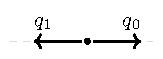
\includegraphics[width=\textwidth]{imgs/classical_cfd/D1Q2.pdf}
         \caption{D1Q2 lattice discretization.}
         \label{subfig:1aa}
     \end{minipage}
     \hfill
          \begin{minipage}{0.45\textwidth}
         \centering
         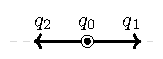
\includegraphics[width=\textwidth]{imgs/classical_cfd/D1Q3-2.pdf}
         \caption{D1Q3 lattice discretization.}
         \label{subfig:1ba}
     \end{minipage}
    \caption{Two examples of different types of D$d$Q$q$ possible for the 1-dimensional case. Figure \ref{subfig:1aa} portrays the D1Q2 setting and Figure \ref{subfig:1ba} portrays the D1Q3 setting (where a stationary particle can be included).}
     \label{fig:multiple_D1Qm}
\end{figure}

 \begin{figure}
     \centering
     \begin{minipage}{.48\textwidth}
         \centering
         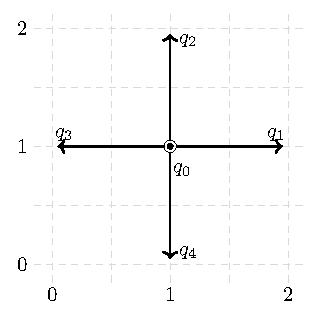
\includegraphics[width=\textwidth]{imgs/classical_cfd/D2Q5.pdf}
         \caption{D2Q5 lattice discretization.}
         \label{subfig:1a-2}
     \end{minipage}
     \hfill
          \begin{minipage}{0.45\textwidth}
         \centering
         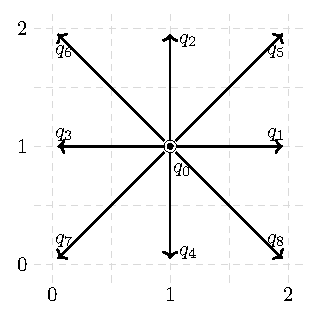
\includegraphics[width=\textwidth]{imgs/classical_cfd/D2Q9.pdf}
         \caption{D2Q9 lattice discretization.}
         \label{subfig:1b-2}
     \end{minipage}
    \caption{Two examples of different types of D$d$Q$q$ possible for the 2-dimensional case. Figure \ref{subfig:1a-2} portrays the D2Q5 setting and Figure \ref{subfig:1b-2} shows the D2Q9 setting. }
     \label{fig:multiple_D2Qm}
\end{figure}


We furthermore write $\mathbf{e}_i$ to represent the vector in the direction $i \in Q=\{0, 1, \dots,q-1\}$ of the D$d$Q$q$ scheme. For example, in the D2Q9 system we have
\begin{equation}
    \mathbf{e}_i = \begin{cases}
      (0,0) & \text{for $i = 0$}\\
      (1,0), (0,1), (-1,0), (0,-1) & \text{for $i = 1,2,3,4$}\\
      (1,1), (-1,1), (-1,-1), (1,-1) & \text{for $i=5,6,7,8$}.
    \end{cases}   
\end{equation}
Therefore $2$ qubits are necessary to represent the speed in each dimension, as the three options `positive', `negative' and `standing still' need to be encoded. 

\subsection{The collisionless Boltzmann equation}
Throughout these lecture notes, we consider the special case that no external forces are present, i.e., $\mathbf{F}=\mathbf{0}$. Moreover, in this section we neglect the collision of molecules to arrive at the collisionless Boltzmann equation
\begin{equation}
  \frac{\partial f}{\partial t} + \mathbf{u}\cdot \nabla f = 0.
  \label{eq:collisionless_boltzmann}
\end{equation}

We assume that the speeds are discrete, i.e., $u^{(i)}\in\mathcal{U}^{(i)}=\{u_1,\dots ,u_{N_{v_i}}\}$. For the scope of these lecture notes we only consider velocities $\mathbf{u}=(u^{(1)},u^{(2)},u^{(3)})$, for which the relative difference in speed in the different dimensions is bounded by
\begin{equation}
    c_\text{rel} = \max \frac{|u^{(i)}|}{|u^{(j)}|}\leq 1.
\end{equation}
As detailed in Section \ref{ssec:class_reflection} this is not a conceptual limitation of our approach, but helps us to keep the number of corner cases to be considered separately small, which also improves the readability of the material. %Moreover, we will drop the superscript $(i)$ wherever possible to improve readability and remark that all operations involving particle speeds are performed dimension by dimension.

As the main focus of this section is to discuss our quantum algorithm for the collisionless Boltzmann equation (CQBM) we will refrain from presenting the derivation of the macroscopic balance equations and just mention that the conservation laws for mass, momentum, and total energy can be derived from the Boltzmann equation \eqref{eq:boltzmann1} as detailed, for instance, in Chapter 2.5 of \cite{Kremer:2010}.

\subsection{Grid definition and obstacle placement}\label{ssec:grid}
In order to keep track of the temporal evolution of the distribution function $f(\mathbf{x},\mathbf{u},t)$, we first define a computational grid with equidistant grid spacing in all two or three spatial dimensions and assign densities to the volumes centered around the grid points. The grid is set up in a straightforward fashion, and grid points can be identified using the Cartesian coordinates system. Obstacles are subsequently placed in between grid points as depicted in Figure~\ref{fig:grid}.

\begin{figure}[h]
\centering
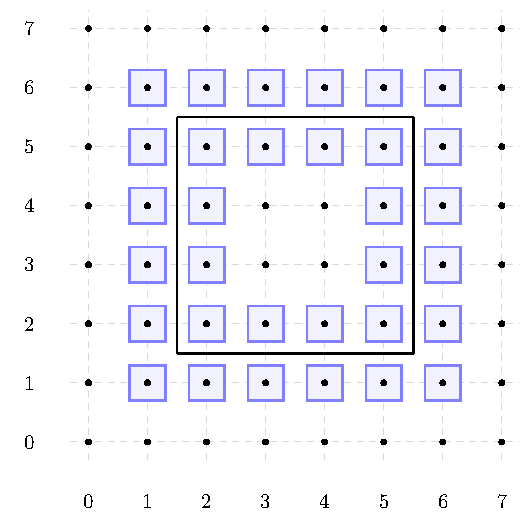
\includegraphics[]{imgs/classical_cfd/grid with obstacle.pdf}
%     \begin{tikzpicture}
%     \draw[help lines, color=gray!30, dashed] (-3.3,-3.3) grid (4.3,4.3);
%     \draw[thick,-,color=black] (-1.5,-1.5) -- (-1.5,2.5);
%     \draw[thick,-,color=black] (-1.5,-1.5) -- (2.5,-1.5);
%     \draw[thick,-,color=black] (2.5,-1.5) -- (2.5,2.5);
%     \draw[thick,color=black] (-1.5,2.5) -- (2.5,2.5);
    
%     \foreach \j in {0,...,3}
%     {
%         \node at (-1+\j,-1)[rectangle, draw=blue!50, fill=blue!5, thick, minimum size=0.6cm]{};
%         \node at (-1+\j,2)[rectangle, draw=blue!50, fill=blue!5, thick, minimum size=0.6cm]{};
%         \node at (-1,-1+\j)[rectangle, draw=blue!50, fill=blue!5, thick, minimum size=0.6cm]{};
%         \node at (2,-1+\j)[rectangle, draw=blue!50, fill=blue!5, thick, minimum size=0.6cm]{};
        
%     }
    
%     \foreach \j in {0,...,5}
%     {
%         \node at (-2+\j,-2)[rectangle, draw=blue!50, fill=blue!5, thick, minimum size=0.6cm]{};
%         \node at (-2+\j,3)[rectangle, draw=blue!50, fill=blue!5, thick, minimum size=0.6cm]{};
%         \node at (-2,-2+\j)[rectangle, draw=blue!50, fill=blue!5, thick, minimum size=0.6cm]{};
%         \node at (3,-2+\j)[rectangle, draw=blue!50, fill=blue!5, thick, minimum size=0.6cm]{};
        
%     }

%     \foreach \j in {0,...,7}
%     {
%         \foreach \i in {0,...,7} 
%         {
%             \node at (-3+\i,-3+\j)[circle, fill, color = black, inner sep=1pt]{};
%         }
%   }
   
%   \foreach \j in {0,...,7}
%   {
%         \node at (-4,-3+\j)[]{\j};
%         \node at (-3+\j,-4)[]{\j};
%   }



%     \end{tikzpicture}
    \caption{Illustration of an obstacle (black box) placed in a computational grid in two dimensions. The grid points (`$\cdot$' surrounded by blue boxes) surrounding the obstacle placement require special attention in our implementation. }
    \label{fig:grid}
\end{figure}

\subsection{Streaming}
In what follows we describe how to move the particles through space.
In the collisionless quantum Boltzmann method not all particles necessarily move in each time step. 
Furthermore, when a particle moves it does not necessarily move in all dimensions in the same time step. The velocity of each particle consists of a speed in each spatial dimension. Whether or not a particle will move in a given dimension depends on the speed in that dimension and whether or not a particle traveling at that speed will reach the next grid point in the current time step. 
This is due to the fact that we choose the size $\Delta t_m$ of time step $m$ to be such that some particles make it to the next grid point, but none overshoot. 
To make this idea more precise we define $u_\text{max} = \max_k |u_k|$ and $u_\text{min} = \min_k |u_k|$, with $u_k \in \mathcal{U} \coloneqq \bigcup_{i=1}^d \mathcal{U}^{(i)}$ the set of possible speeds a particle can travel. Then, we can normalize the distance between the grid points $\Delta x$ to enforce it will always be equal to $1$. Subsequently, the first time step $\Delta t_0$ will have size $\frac{1}{u_\text{max}}$. All particles that travel with speed $\pm u_{\text{max}}$ in a dimension will move one grid point in the first time step in that dimension. To determine the size $\Delta t_m$ of any subsequent time step $m$, we keep track of the distances a particle traveling at any of the possible speeds $u_k\in\mathcal{U}$ would be removed from reaching the next grid point and use this to find the smallest time step necessary for any particle to reach the next grid point in any dimension.

To ensure that particles can travel no further than the neighboring grid points, and thereby adhere to the CFL (Courant-Friedrichs-Lewy) condition, we use a so called CFL counter. This counter keeps track of the distances the particles are located from the next grid point based on their speed in each dimension and thereby determines the size of the next time step. 


\subsubsection{CFL counter}\label{ssec:cfl_counter}
In what follows, let $c^m_k$ represent how large of a fraction from the current grid point to the next a particle with speed $u_k$ has to travel.
We use the following expression
\begin{equation}
    c^{m+1}_{k} = c^m_{k} + |u_k| \frac{\Delta t_m}{\Delta x},
\end{equation}
where $u_k \in \mathcal{U}$ and $m$ represents the number of time steps that have been taken so far. Furthermore, $\Delta x$ represents the equidistant spacing between the grid points as before.  
It then follows that we can express the size of the time step taken in each iteration as
\begin{equation}\label{eq:delta_t}
    \Delta t_m = \min_{k} \left ( \left [1-c^m_{k} \right ] \frac{\Delta x}{|u_k|}  \right ).
\end{equation}
In the above equation we minimize over $k$ to ensure that at least one speed reaches the next grid point, and none overshoots. 

In a classical Boltzmann method $c_k^{m}$ can be used to interpolate the results when the simulation terminates in a time step that is not a complete cycle. This is not possible in the quantum counterpart and thus if we terminate the simulation in a time step that is not a complete cycle, some small oscillations will occur unless a post-smoothing method is applied. In this manuscript we restrict ourselves to running the CQBM algorithm for a total time $T = \sum_{m=0}^{N_t -1} \Delta t_m$ such that $\frac{T}{u_m} \in \mathbb{Z}$ $\forall m$. 

To complete the collisionless quantum Boltzmann method we need to describe the behavior when a particle collides with an obstacle. 

\subsection{Collision}
The collision step in the Boltzmann method is usually performed by taking a collision operator, such as the BGK operator \cite{Bhatnagar1954}, and performing a relaxation towards equilibrium. In these notes we will introduce the idea of equivalence classes, as used in the lattice gas models of the last century \cite{Yepez1998}. Two combinations of velocities belong to the same equivalence class if the resulting momentum is the same. Figure \ref{fig:equivalence_class} shows two combinations of velocities that belong to the same equivalence class for the D2Q5 case.

 \begin{figure}
     \centering
     \begin{minipage}{.48\textwidth}
         \centering
         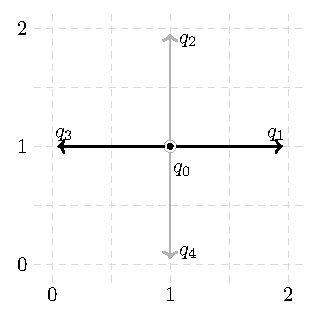
\includegraphics[width=\textwidth]{imgs/classical_cfd/equivalence_class_1.pdf}
         \caption{Equivalence class depiction for D2Q4 lattice discretization.}
         \label{subfig:1a}
     \end{minipage}
     \hfill
          \begin{minipage}{0.45\textwidth}
         \centering
         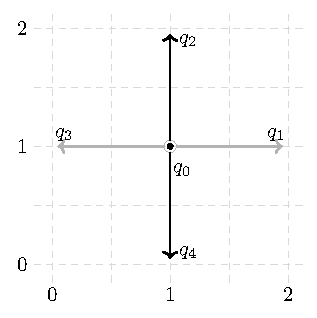
\includegraphics[width=\textwidth]{imgs/classical_cfd/equivalence_class_2.pdf}
         \caption{Equivalence class depiction for D2Q4 lattice discretization.}
         \label{subfig:1b}
     \end{minipage}
    \caption{Illustration of two velocity combinations of the D2Q5 (and D2Q4) velocity spectrum that belong to the same equivalence class with total momentum 0 and mass 2: (a) particles streaming in the $q_1$ and $q_3$ direction, and (b) particles streaming in the $q_2$ and $q_4$ direction. }
\label{fig:equivalence_class}
\end{figure}



\subsection{Reflection by an obstacle}\label{ssec:class_reflection}
In specular reflection, when a particle impinges on an object its velocity gets reflected along the axis normal to that object. 
Notice that due to this method we are restricted to modeling objects whose walls are either parallel or perpendicular to each dimension.
In order to facilitate the correct reflections we need to keep track of when a particle has come into contact with a wall, this is done differently for different values of $c_\text{rel}$.

We first consider the case $c_\text{rel} \leq 1$. In this case we know a particle has come into contact with an object if and only if it hits a grid point located in the first layer of the obstacle. We will refer to these grid points as the wall of the object. When a particle reaches a grid point in the wall of an object, its velocity normal to the wall gets reversed and the particle is moved one grid point outside of the object again in the direction normal to the wall(s) that just reflected it. Figure \ref{fig:specular reflection} gives an example of what such a reflection might look like.

\begin{figure}
\centering
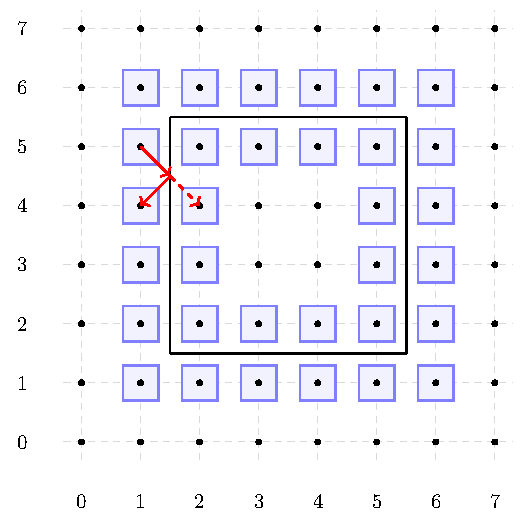
\includegraphics[]{imgs/classical_cfd/grid with reflection.pdf}
%     \begin{tikzpicture}
%     \draw[help lines, color=gray!30, dashed] (-3.3,-3.3) grid (4.3,4.3);
%     \draw[thick,color=black] (-1.5,-1.5) -- (-1.5,2.5);
%     \draw[thick,color=black] (-1.5,-1.5) -- (2.5,-1.5);
%     \draw[thick,color=black] (2.5,-1.5) -- (2.5,2.5);
%     \draw[thick,color=black] (-1.5,2.5) -- (2.5,2.5);
    
    
%     \foreach \j in {0,...,3}
%     {
%         \node at (-1+\j,-1)[rectangle, draw=blue!50, fill=blue!5, thick, minimum size=0.6cm]{};
%         \node at (-1+\j,2)[rectangle, draw=blue!50, fill=blue!5, thick, minimum size=0.6cm]{};
%         \node at (-1,-1+\j)[rectangle, draw=blue!50, fill=blue!5, thick, minimum size=0.6cm]{};
%         \node at (2,-1+\j)[rectangle, draw=blue!50, fill=blue!5, thick, minimum size=0.6cm]{};
        
%     }
    
%     \foreach \j in {0,...,5}
%     {
%         \node at (-2+\j,-2)[rectangle, draw=blue!50, fill=blue!5, thick, minimum size=0.6cm]{};
%         \node at (-2+\j,3)[rectangle, draw=blue!50, fill=blue!5, thick, minimum size=0.6cm]{};
%         \node at (-2,-2+\j)[rectangle, draw=blue!50, fill=blue!5, thick, minimum size=0.6cm]{};
%         \node at (3,-2+\j)[rectangle, draw=blue!50, fill=blue!5, thick, minimum size=0.6cm]{};
        
%     }
    
    
%     \foreach \j in {0,...,7}
%     {
%         \foreach \i in {0,...,7} 
%         {
%             \node at (-3+\i,-3+\j)[circle, fill, color = black, inner sep=1pt]{};
%             \node at (-3+\i,-3+\j)[circle, fill, color = black, inner sep=1pt]{};
%         }
%   }
%     \draw[->,color=red, thick] (-2,2) -- (-1.5,1.5);
%     \draw[->,dashed,color=red, thick] (-1.5,1.5) -- (-1,1) ;
%     %\draw[->,dashed,color=red, thick] (-1,1) -- (-1.5,0.5) ;
%     \draw[->,color=red, thick] (-1.5,1.5) -- (-2,1);
%     %\draw[->,dashed,color=red, thick] (-2,1) -- (-2.5,0.5) ;
    
%   \foreach \j in {0,...,7}
%   {
%         \node at (-4,-3+\j)[]{\j};
%         \node at (-3+\j,-4)[]{\j};
%   }

%     \end{tikzpicture}
    \caption{Illustration of an obstacle (black box) in the grid with the red arrow representing one possible collision operation. The dashed arrow represents the trajectory had no reflection taken place. }
    \label{fig:specular reflection}
\end{figure}

For $c_\text{rel} > 1$ the specular reflection step becomes more complicated, as grid points located outside the object can be reached by a particle indicating that the particle has come into contact with an object; See Figure \ref{fig:specular reflection c3}. Similarly multiple cases need to be taken into account to determine whether a particle hits a corner point of an object or the wall at a non-corner point. For simplicity we will restrict ourselves to the case $c_\text{rel} \leq 1$ for the scope of this paper, but we would like to remark that our method can be generalized to any value of $c_\text{rel}$ at the cost of taking into account more corner cases.

\begin{figure}
\centering
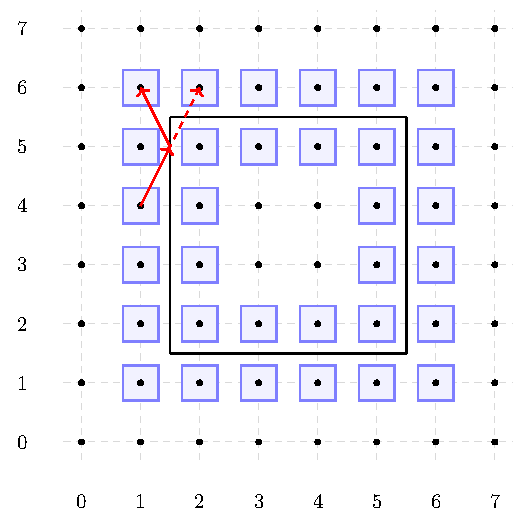
\includegraphics[]{imgs/classical_cfd/grid with reflection crel.pdf}
%     \begin{tikzpicture}
%     \draw[help lines, color=gray!30, dashed] (-3.3,-3.3) grid (4.3,4.3);
%     \draw[thick,color=black] (-1.5,-1.5) -- (-1.5,2.5);
%     \draw[thick,color=black] (-1.5,-1.5) -- (2.5,-1.5);
%     \draw[thick,color=black] (2.5,-1.5) -- (2.5,2.5);
%     \draw[thick,color=black] (-1.5,2.5) -- (2.5,2.5);
    
    
%     \foreach \j in {0,...,3}
%     {
%         \node at (-1+\j,-1)[rectangle, draw=blue!50, fill=blue!5, thick, minimum size=0.6cm]{};
%         \node at (-1+\j,2)[rectangle, draw=blue!50, fill=blue!5, thick, minimum size=0.6cm]{};
%         \node at (-1,-1+\j)[rectangle, draw=blue!50, fill=blue!5, thick, minimum size=0.6cm]{};
%         \node at (2,-1+\j)[rectangle, draw=blue!50, fill=blue!5, thick, minimum size=0.6cm]{};
        
%     }
    
%     \foreach \j in {0,...,5}
%     {
%         \node at (-2+\j,-2)[rectangle, draw=blue!50, fill=blue!5, thick, minimum size=0.6cm]{};
%         \node at (-2+\j,3)[rectangle, draw=blue!50, fill=blue!5, thick, minimum size=0.6cm]{};
%         \node at (-2,-2+\j)[rectangle, draw=blue!50, fill=blue!5, thick, minimum size=0.6cm]{};
%         \node at (3,-2+\j)[rectangle, draw=blue!50, fill=blue!5, thick, minimum size=0.6cm]{};
        
%     }
    
%     % \foreach \j in {0,1}
%     % {
%     %     \foreach \i in {0,1}
%     %     {
%     %     \node at (-3+2 + 3*\j,-2+5*\i)[rectangle, draw=green!50, fill=blue!5, thick, minimum size=0.6cm]{};
%     %     \node at (-2+5*\i,-3+2 + 3*\j)[rectangle, draw=orange!50, fill=blue!5, thick, minimum size=0.6cm]{};
%     %     }
%     % }
    
%     \foreach \j in {0,...,7}
%     {
%         \foreach \i in {0,...,7} 
%         {
%             \node at (-3+\i,-3+\j)[circle, fill, color = black, inner sep=1pt]{};
%             \node at (-3+\i,-3+\j)[circle, fill, color = black, inner sep=1pt]{};
%         }
%   }
%     \draw[->,color=red, thick] (-1.5,2) -- (-2,3) ;
%     \draw[->,color=red, thick] (-2,1) -- (-1.5,2) ;
%     \draw[->,dashed,color=red, thick] (-2,1) -- (-1,3) ;
    
%   \foreach \j in {0,...,7}
%   {
%         \node at (-4,-3+\j)[]{\j};
%         \node at (-3+\j,-4)[]{\j};
%   }

%     \end{tikzpicture}
    \caption{Illustration of an obstacle (black box) in the grid with the red arrow representing one possible specular reflection operation when $c_\text{rel} > 1$ holds. The dashed arrow represents the trajectory had no reflection taken place. }
    \label{fig:specular reflection c3}
\end{figure}

\section{Momentum Exchange Method}\label{sec:MEM}
The momentum exchange method was proposed by Ladd \cite{Ladd1994} to determine the force acting on an object in order to calculate the drag and lift coefficients of an obstacle equipped with bounce back boundary conditions when the flow field is modelled by the Boltzmann method. Bounce back boundary conditions differ from the more intuitive specular reflection boundary conditions in that, upon contact with an object, the particle's velocity is reversed entirely instead of just the velocity normal to the object; see Figure \ref{fig:bounce_back_vs_specular_reflection}. Bounce back boundary conditions are often used in combination with the Lattice Boltzmann method \cite{Kruger2017}. In Section \ref{sec:qbb} we give an in-depth explanation of bounce back boundary conditions as well as how to implement them in our QLBM scheme.
In this paper we adopt the momentum exchange method as described in \cite{Kruger2017}. Then the force exerted on the object by the particles can be expressed as
\begin{equation}\label{eq:F1}
    \mathbf{F} = \sum_{i\in Q} \left ( \mathbf{e}_{i}f_i(\mathbf{x}_f,t) - \mathbf{e}_{\bar{i}} f_{\bar{i}}(\mathbf{x}_f,t) \right ) .
\end{equation}
In the above expression $\mathbf{x}_f$ refers to a point in the fluid space adjacent to the obstacle and $\bar{i}$ represents the velocity of the particles after particles with velocity $i$ have impinged on the object.
$Q$ is the set of all distinct velocities in the discretization.
This expression assumes that there is no fluid inside the object and as such only takes the momentum exchange outside of the object into account. Since we are using bounce back boundary conditions we have $\mathbf{e}_{\bar{i}}:=-\mathbf{e}_i$ and
$f_i(\mathbf{x}_f,t) = f_{\bar{i}}(\mathbf{x}_f,t)$ by definition, therefore we can rewrite Equation \eqref{eq:F1} to 
\begin{equation}\label{eq:F2}
    \mathbf{F} = \sum_{i\in Q} 2 \mathbf{e}_{i} f_i(\mathbf{x}_f,t).
\end{equation}
As force is composed of magnitude and direction it is expressed by a $d$ dimensional vector with subscript $j$ denoting its $j$-th dimensional component, i.e.
\begin{equation}\label{eq:F2_d}
    F_j = \left ( \sum_{i\in Q} 2 \mathbf{e}_{i} f_i(\mathbf{x}_f,t) \right )_j.
\end{equation}

% =============================================================================
\section{Collisionless quantum lattice Boltzmann method \label{sec:cqbm}}
In this chapter we will introduce the reader to our quantum implementation of the collisionless lattice Boltzmann method. We will first describe how the equation can be encoded in the quantum register, and subsequently we will provide the quantum primitive for the streaming, specular reflection and bounce back step. 

\subsection{Quantum register set-up}\label{sec:quantum register set-up}
In order to implement our CQBM approach we first need to define an encoding to give a physically interpretable meaning to quantum basis states. 
In our implementation we define a mapping, where each parameter is assigned to its own set of qubits, which combined form the total qubit register. 
We use the following encoding:
% \begin{equation}
%     \ket{a_{2d} \dots a_1 l_{dN_d} \dots l_{d1} \dots l_{xN_x} \dots l_{x1} v_{N_v} \dots v_1 }
% \end{equation}
\begin{equation}
    \ket{\underbrace{a_{n_a}\dots a_{1}}_{\mathrm{ancillae}} \overbrace{ g_{n_g} \dots g_{1} }^{\mathrm{position}} \underbrace{ v_{n_v} \dots v_1}_{\mathrm{velocity}}}.
\end{equation}

Here, the qubits $a_{n_a}, \dots, a_1$ form the ancillae, with $n_a = 4d-2$, where $d$ is the number of spatial dimensions we are modeling. The $g_{n_g} \dots g_1$ qubits form the positional qubits, with $n_g = \sum_{i=1}^{d}n_{g_i}$, where $n_{g_i}$ is the number of qubits required to number all grid points in the $i$-th spatial dimension. Finally, the qubits $v_{n_v} \dots v_1$ encode the velocity vector, with $n_v = \sum_{i=1}^{d}n_{v_i} $ where $n_{v_i}$ is the number of qubits required number the velocities of the $i$-th dimension. In summary, the total number of qubits required to realize our collisionless quantum Boltzmann method is
\begin{equation}
    a_n + n_g + n_v = 4d-2 + \sum_{i=1}^d (n_{g_i}+n_{v_i}),
\end{equation}
which means that a moderate number of a few dozens to hundred fault-tolerant qubits suffice to enable the solution of two and three-dimensional problems.
The details of the mapping of the ancillae, positional and velocity vectors will be explained more in depth in the following sections. 


\subsubsection{Efficient mapping of velocity vector}
One of the speed-ups our algorithm provides compared to the state-of-the-art is due to our mapping of the velocity vector. 
In each spatial dimension we are working with a predetermined number of discrete velocities $N_{v_i}$. 
For simplicity we will at first only consider the velocity encoding in the one-dimensional case, and call the amount of discrete velocities $N_{v}$. Note that this approach trivially extends to the multi-dimensional case.
As $N_v$ is the number of discrete velocities required, we need $n_{v} = \lceil\log_2\left(N_v\right)\rceil$ qubits to encode all velocities. \\
For our CQBM we restrict ourselves to the case that the set of speeds $\mathcal{U}$ consists of positive and negative values, and for each $u\in \mathcal{U}$ both $|u|\in \mathcal{U}$ and $-|u|\in \mathcal{U}$ will hold. We now define $\mathcal{U}_o = [-u_{\max}, \dots , u_{\max} ]$, the ordered list of speeds from most negative to most positive. 
Let $u_{\min} = \min_k \; |u_k| $ as before and let $\Delta u $ be the distance between the neighboring speeds in $\mathcal{U}_o$, for simplicity we will assume $\Delta u$ is constant between all indices so $\Delta u=\frac{2u_{\max}}{N_v}$. However, we are not restricted to this simplification.  \\
% In the state-of-the-art quantum finite velocity methods (@MATTHIAS, welke term kan ik hier het beste gebruiken) \cite{Todorova2020}, the discrete velocities are mapped to the quantum states as follows: 
% \begin{equation}\label{eq:old_v_encoding}
% \ket{v_{old}} = 
%     \begin{bmatrix}
%     -c_{max} \\
%     -c_{max} +\Delta c  \\
%     \vdots \\
%     -c_{min} \\
%     c_{min}\\
%     c_{min} +\Delta c  \\
%     \vdots \\
%     c_{max}\\
%     \end{bmatrix}.
% \end{equation}
% In such algorithms the velocities are required to control streaming operations and the direction of the velocity needs to be reversed when a particle hits a wall (i.e. $v_i$ becomes $-v_i$). As these are the two requirements, a more efficient encoding of the velocity mapping is possible which saves $\mathcal{O}(n_v)$ multi-controlled not operations in the reflection step. 
% This is due to the fact that in the current implementation, in order to reverse a velocity (i.e. going from the basis state encoding $v_i$ in \eqref{eq:old_v_encoding} to the basis state encoding $-v_i$), each qubit needs to be flipped \cite{Todorova2020}. 
% In practical algorithms such a reversal of velocity needs to be done in a multi-controlled fashion, making each qubit flip rather expensive. \\

We propose the following mapping of the discrete velocities to the quantum state:
\begin{align}
\ket{v_{n_v} \dots v_1} = 
    \begin{bmatrix}
    -u_{\min} \phantom{\, -\Delta u}\\
    -u_{\min} -\Delta u\\
    \vdots \\
    -u_{\max} \phantom{\, -\Delta u}\\
    \phantom{-}u_{\min} \phantom{\, -\Delta u}\\
    \phantom{\,-}u_{\min} +\Delta u  \\
    \vdots \\
    \phantom{-}u_{\max} \phantom{\, +\Delta u}\\
    \end{bmatrix}.\label{eq:our_v}
\end{align}
The motivation of this velocity mapping is that we can flip the direction of the velocity by flipping only one qubit. This can be seen by noting that the distance between the index of velocity $-|u_k|$ and $|u_k|$ in $\mathcal{U}_o$ is precisely $\frac{N_v}{2} = 2^{n_v-1}$, and so we can flip between these two velocities by flipping the most significant qubit which encodes the sign of the velocity vector.% as that represents exactly the $\frac{N_v}{2} = 2^{n_v-1}$ value in binary.\\

This means that we can write the quantum register encoding the velocity in the one dimensional case as: 
\begin{equation}
   \ket{v_{\text{dir}} v_{n_v -1} \dots v_1}.
\end{equation}
In the above expression the first qubit encodes the direction of the velocity (positive or negative in the given dimension), and the next $n_v-1$ qubits encode the magnitude of the velocity. We define $\ket{00 \dots 0}$ to encode $-u_{\min}$, $\ket{00 \dots 1}$ to encode $-u_{\min} - \Delta u$ and $\ket{11 \dots 1}$ to represent $u_{\max}$ etc. It can easily be seen that this leads to a velocity encoding as given in Equation \eqref{eq:our_v}.

\paragraph{Example}\
\normalem
\emph{We give an example of our velocity encoding to show that flipping the direction can be established by flipping only the most significant qubit. Let us consider the 1-dimensional case and say we have $N_v = 8$. Now let $u_1 = u_{\min}$, $u_2 = u_{\min} + \Delta u$ and $u_3 = u_{\min} + 2\Delta u$ etc., then our velocity encoding gives $$\ket{v} = \begin{bmatrix}
-u_1 \\ -u_2\\ -u_3 \\ -u_4\\ \phantom{-}u_1 \\ \phantom{-}u_2\\ \phantom{-}u_3 \\ \phantom{-}u_4 
\end{bmatrix}.$$ Say our particle is traveling with velocity $u_2$, then $\ket{v} = \ket{101}$. Now flipping the most significant qubit gives $\ket{v} = \ket{001}$ which maps to $-u_2$ as required. }\\
% \emph{We will now give an example of our velocity encoding method to show that flipping the velocity direction can be established by flipping only the most significant qubit. Let us consider the 1-dimensional case and say we have $N_v = 8$, then we can encode $\ket{v} = \begin{bmatrix}
% -u_\text{min} \\ -u_\text{min} - \Delta u \\ -u_\text{min} -2\Delta u \\ -u_\text{max} \\ u_\text{min}  + \Delta u \\ u_\text{min} + 2\Delta u \\ u_\text{min} + 3\Delta u \\ u_\text{max}
% \end{bmatrix}$ . Now say our particle is traveling with velocity $u_2$, then $\ket{v} = \ket{101}$, now flipping the most significant bit gives $\ket{v} = \ket{001}$ which maps to $-u_2$. }\\

\ULforem
Extending the above approach to the multidimensional case, the quantum register for the $d$-dimensional velocity becomes: 
\begin{equation}
\ket{v_{\text{dir},d} \dots v_{\text{dir},1} v^d_{n_{v_d}} \dots v^d_{1} v^{d-1}_{n_{v_{d-1}}} \dots v^{d-1}_{1} \dots v^1_{n_{v_1}} \dots v^1_{1}} . 
\end{equation}

Former encodings of the velocity vector for quantum Boltzmann methods were set-up such that in order to flip the velocity of a particle, all qubits encoding the velocity needed to be flipped \cite{Todorova2020}. Our new encoding saves $\mathcal{O}\left ( n \right )$ qubit flips per reflection. Notice that since reflections are usually implemented in multi-control fashion, as described in Section \ref{sec:complete quantum specular reflection step}, this ends up in saving $\mathcal{O}\left (n \right )$ computationally costly operations per reflection. In the appendix we give an in depth complexity analysis and comparison of the different methods.

\subsubsection{Mapping of grid point locations onto qubit states}
The mapping of the grid point locations onto qubit states is rather straightforward. As before, let $\ket{g_{n_g} \dots g_1}$ represent the state of the qubits encoding the grid point location of the particles. Then, we can write the qubits encoding the location more detailed as
\begin{equation}
\ket{g^d_{n_{g_d}} \dots g^d_{1} g^{d-1}_{n_{g_{d-1}}} \dots g^{d-1}_{1} \dots  g^1_{n_{g_1}} \dots g^1_{1}},
\end{equation}
where $g^i_{n_{g_i}} \dots g^i_{1} $ encodes the $i$-th dimension of the location of grid points by representing the binary value of the location. The set-up of the grid is rather straightforward with different grid-points in each dimension and the particles being able to move one step forward and backward in each time step and in each dimension. 


\subsubsection{Ancillae}
The ancillae are the last of the register expressed in Equation \eqref{eq:our_v} and are used within the computation only. 
Each dimension requires one ancilla to keep track of which velocities will be streamed and one ancilla to keep track of the resetting
during the reflection step, furthermore we require $2(d-1)$ ancillae to implement a quantum comparator method that will be used in the reflection step, leading to a total of $4d-2$ ancillae required throughout the computation.
The exact set-up and utilization of the ancillae will be described in Sections \ref{sec:efficient quantum convection operation} and \ref{sec:complete quantum specular reflection step}. 


\subsection{Efficient quantum streaming operation}\label{sec:efficient quantum convection operation}
As described in Section \ref{sec:collisionless boltzmann equation2} the main ingredients of the collisionless quantum Boltzmann method are the streaming and the reflection operations. In this section we will introduce a novel streaming operation based on the Quantum Draper Adder \cite{Draper1998}, which we specialize to an efficient quantum incrementation (decrementation) procedure that is cheaper than those used before \cite{Douglas2009,Fillion-Gourdea2017, Fillion-Gourdea2018,Todorova2020}. \\

\subsubsection{Efficient quantum incrementation (decrementation)}\label{ssec:efficient quantum incr}
An increment (decrement) operation takes a quantum state $\ket{j}$ to the state $\ket{j+1}$ $\left (\ket{j-1} \right )$. This operation is cyclic, meaning that $\ket{2^n-1}$ ($\ket{0}$) gets incremented (decremented) to $\ket{0}$ $\left (\ket{2^n-1} \right )$.  
Let $U_\text{inc}$ ($U_\text{dec}$) express the unitary that increases (decreases) the $n$ qubit state $\ket{j}$: 
\begin{equation}
    U_\text{inc} \ket{j} = \ket{j+1},
\end{equation}
\begin{equation}
    U_\text{dec} \ket{j} = \ket{j-1}.
\end{equation}
This quantum primitive is used in many different quantum algorithm and fields such as Quantum Random Walks and Quantum Computational Fluid Dynamics, to name just a few. In the literature this primitive is typically implemented by cascading multi-controlled NOT operations \cite{Douglas2009,Fillion-Gourdea2017, Fillion-Gourdea2018,Todorova2020, Budinski2021}. While this implementation looks elegant on paper, decomposing multi-controlled NOT operations into gates that are native to quantum computers, i.e., single-controlled NOT gates, will lead to a significant increase of the circuit depth. 

In this section we provide an alternative method leading to a quantum streaming operation which can be implemented more efficiently on real-world quantum computers. The method is inspired by the Quantum Draper Adder (QDA) \cite{Draper1998} and uses the same principle, but in contrast to the regular Drapper adder that computes $\ket{a + b}$, where $a$ and $b$ are natural numbers encoded in a quantum register, in our implementation the phase shift operations are not controlled as the addition by $b=1$ is always known beforehand. As we moreover want our operation to be cyclic, no qubit for holding a potential carry over value is required. We are, to the best of our knowledge, the first to use such a QDA inspired approach for the quantum incrementer (decrementer) and the Appendix we show that it leads to a significant reduction in the amount of CNOT gates required to run the algorithm. \\

Our method can be expressed by the circuit given in Figure \ref{fig:streaming_no_anc}. 
Let $\ket{j}$ be the basis state that we wish to increment (decrement). We claim
\begin{equation} \label{eq:our_adder}
    \ket{j+1} = (QFT)^\dagger U_{P,+} (QFT) \ket{j},
\end{equation} and define 
\begin{equation} \label{eq:def our_adder}
    U_\text{inc}= (QFT)^\dagger U_{P,+} (QFT),
\end{equation} where QFT stands for Quantum Fourier Transform and $U_{P,+}$ will be defined below.
We will now show that \eqref{eq:our_adder} indeed holds. First: 
\begin{equation}
    QFT \ket{j} = \frac{1}{\sqrt{N}}\sum_{k=0}^{N-1} \omega_N^{kj}\ket{k} = \frac{1}{\sqrt{N}} \sum_{k=0}^{N-1} e^{\frac{2 i \pi k j}{N}}\ket{k}.
\end{equation}
Then the circuit $U_{P,+}$ consists of one phase shift gate\footnote{The single qubit phase shift gate can be expressed in matrix form as $P\left ( \theta \right ) = \begin{bmatrix}1 & 0 \\ 0 & e^{i\theta} \end{bmatrix}$.  } per qubit with an angle determined by the qubit number of the qubit to which it is applied. We apply the phase shift gate $P(\theta)$ to the $j$-th qubit\footnote{In this section, for simplicity, we index the qubits ranging from 0 to $n-1$.} with angle
\begin{equation}\label{eq:theta_i}
    \theta_j=\frac{\pi}{2^{n-1-j}} =\frac{\pi 2^{j+1}}{N}.
\end{equation}

So $P(\theta_j)$ gets applied to qubit $j$ and adds amplitude $e^{\frac{i2\pi 2^j}{N}}$ to each basis state for which qubit $j$ is in the state $1$. This means that if we apply the operation $P(\theta_j)$ to each qubit for the basis state $\ket{k}$ it gets multiplied by a factor $e^{\frac{2\pi i k}{N}}$. 

And so we get: 
\begin{equation}
    U_{P,+} (QFT) \ket{j} = \frac{1}{\sqrt{N}} \sum_{k=0}^{N-1} e^{\frac{2 i \pi k j}{N}}e^{\frac{2\pi i k}{N}} \ket{k} = \frac{1}{\sqrt{N}} \sum_{k=0}^{N-1} e^{\frac{2 i \pi k (j+1)}{N}}\ket{k} .
\end{equation}

It then directly follows that: 
\begin{equation}
    (QFT)^\dagger U_{P,+} (QFT) \ket{j} = QFT^\dagger \frac{1}{\sqrt{N}} \sum_{k=0}^{N-1} e^{\frac{2 i \pi k (j+1)}{N}}\ket{k}  = \ket{j+1}.
\end{equation}
In other words our proposed algorithm increases each basis state by $1$, whereby the periodic property of $e^{i\theta}$ ensures that the so-defined increase operation is cyclic. Naturally the decrease operation becomes:
\begin{equation}
    \ket{j} =  \left ( (QFT)^\dagger U_{P,+} (QFT) \right )^\dagger \ket{j+1} = (QFT)^\dagger U_{P,+}^\dagger (QFT) \ket{j+1}.
\end{equation}
Since $U_{P,+}$ consists of a layer of phase shift gates taking the conjugate transpose is equal to shifting the angles to their negative counterparts. So for $U_{P,+}^\dagger$ we apply the phase shift gate $P(-\theta_j)$ to the $j$-th qubit with angle $-\theta_j$, where $\theta_j$ is as given in \eqref{eq:theta_i}.
For simplicity we define $U_{P,-} = U_{P,+}^\dagger$. It then follows that: 
\begin{equation}
    U_{\text{dec}} = (QFT)^\dagger U_{P,-} (QFT).
\end{equation}
 



% \subsection{Proposed incrementation (decrementation) method}
% Our incrementation method can be expressed by the circuit as given in figure \ref{}. 
% Let $\ket{j}$ be the basis state to which we apply the qubit, the we claim: 
% \begin{equation} \label{eq:our_adder}
%     \ket{j+1} = QFT^\dagger U_P QFT \ket{j}.
% \end{equation}

% We will now show that \eqref{eq:our_adder} holds. First: 
% \begin{equation}
%     QFT \ket{j} = \frac{1}{\sqrt{N}}\sum_{k=0}^{N-1} \omega_N^{kj}\ket{k} = \frac{1}{\sqrt{N}} \sum_{k=0}^{N-1} e^{\frac{2 i \pi k j}{N}}\ket{k}.
% \end{equation}
% Then the circuit $U_P$ consists of one phase shift gate per qubit with an angle determined by which qubit it is applied to. We apply the phase shift gate $P(\theta)$ to the $i$-th qubit with angle
% \begin{equation}
%     \theta_i=\frac{\pi}{2^{n-1-i}} =\frac{2\pi 2^i}{N}.
% \end{equation}

% So $P(\theta_i)$ gets applied to qubit $i$ and adds amplitude $e^{\frac{2\pi 2^i}{N}}$ to each basis state for which qubit $i$ is in the state $1$. This means that if we apply this operation $P(\theta_i)$ to each basis state $\ket{k}$ it gets multiplied by a factor $e^{\frac{2\pi i k}{N}}$. 

% And so we get: 
% \begin{equation}
%     U_P QFT \ket{j} = \frac{1}{\sqrt{N}} \sum_{k=0}^{N-1} e^{\frac{2 i \pi k j}{N}}e^{\frac{2\pi i k}{N}} \ket{k} = \frac{1}{\sqrt{N}} \sum_{k=0}^{N-1} e^{\frac{2 i \pi k (j+1)}{N}}\ket{k} .
% \end{equation}

% It then directly follows that: 
% \begin{equation}
%     QFT^\dagger U_P QFT \ket{j} = QFT^\dagger \frac{1}{\sqrt{N}} \sum_{k=0}^{N-1} e^{\frac{2 i \pi k (j+1)}{N}}\ket{k}  = \ket{j+1}.
% \end{equation}
% And so our proposed algorithm increases each basis state by $1$. Note that from the periodic properties of $e^{i\theta}$ that this increase operation is cyclic. Naturally the decreasing operation becomes:
% \begin{equation}
%     \ket{j} =  (QFT)^{-1} U_P^{-1} (QFT^\dagger)^{-1} \ket{j+1} = (QFT^\dagger) U_P^\dagger (QFT) \ket{j+1}.
% \end{equation}
% Since $U_P$ consists of a layer of phase shift gates taking the complex conjugate is equal to shifting the angles to their negative counter parts. So for $U_P^\dagger$ we apply the phase shift gate $P(-\theta)$ to the $i$-th qubit with angle
% \begin{equation}
%     \theta_i=\frac{\pi}{2^{n-1-i}} =\frac{2\pi 2^i}{N}.
% \end{equation}




\subsubsection{Streaming step}\label{ssec:convection step}
In the streaming step particles migrate from one discrete point in space to another. 
In each time step the particles that travel at a discrete speed such that they reach the next grid point in the current time step get incremented (or decremented) one position in space. The list of speeds for which particles traveling at that specific speed need to be incremented (decremented) at a particular time step is pregenerated by the CFL counter as described in Section \ref{ssec:cfl_counter}. Then, controlled on their speeds, the particles are incremented (decremented) one position at a time. This means that we implement the quantum incrementation (decrementation) method as described in the last section in a controlled fashion as will be detailed below.  \\

First of all we notice that we do not have to control the entire incrementation (decrementation) primitive from Section \ref{ssec:efficient quantum incr}. Since the incrementation (decrementation) step consists of the QFT followed by a layer of phase shift gates followed by QFT$^\dagger$, it suffices to only control the layer of phase shift gates on the speed of the particles, as the QFT and QFT$^\dagger$ operations naturally cancel out each other. Furthermore, since the incrementation and decrementation step are performed directly after each other on the same qubits, we do not have to perform a QFT$^\dagger$ operation after the phase shift gates of the incrementation step, as this would cancel out with the QFT operation at the start of the decrementation step.  \\

Second, we notice that if we make use of an ancilla we can perform the incrementation and decrementation operations for all speeds that take a step in the current time step using a single operation in a given dimension $i$. 

To this end, let $|u_k|$ be (one of) the absolute values of the speeds for which the streaming step is to be performed at a certain point in the algorithm. Then in each dimension $i$ we need to increment the particles traveling at speed $u^{(i)} = \pm |u_k|$. Because of the way the binary encodings of $u_k$ and $-u_k$ are related in each dimension, we first perform a controlled-NOT operation between the $n_{v_i}-1$ qubits determining the absolute value of the velocity and an ancilla qubit $a_{u,i}$. If there are multiple values $k$ such that particles traveling at speed $\pm u_k$ need to be incremented in the given time step, this process is applied to all such $k$. This means that we simply flip the value of the ancilla qubit $a_{u,i}$ to 1 for all the registers of the particles traveling at a speed such that they should reach the next grid point in dimension $i$ in the current time step. We then use the ancilla $a_{u,i}$ in combination with the directional velocity qubit $v_{\text{dir},i}$ to increase or decrease the position of the correct particles in space in each dimension $i$. 
In practice, the streaming step using the ancilla qubits $a_{u,i}$ should be implemented as it leads to a more efficient algorithm, due to the fact that we now perform the incrementation (decrementation) primitive for all the particles taking a step in the given time step using a single operation. 

\begin{figure}
    \centering
    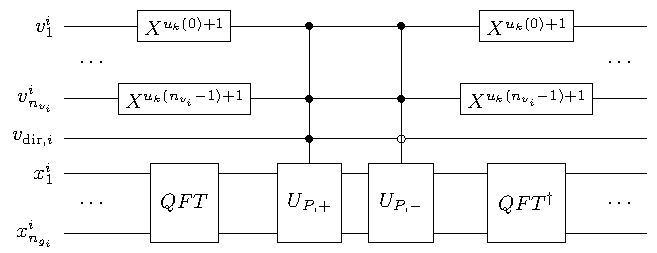
\includegraphics{imgs/cqlbm/streaming no anc_2.pdf}
%     \[\Qcircuit @C=1.3em @R=1em {
% %& & & & & \mbox{Rigetti generated amplitude amplification circuit} & & & & & \\
% &\lstick{v^i_1} & \qw & \gate{X^{u_{k}(0)+1}} & \qw & \ctrl{4} & \ctrl{4} & \qw & \gate{X^{u_{k}(0)+1}} & \qw & \qw\\
% &\lstick{} & \cdots & & & & & & & \cdots & \\
% &\lstick{v^i_{n_{v_i}}} & \qw & \gate{X^{u_{k}(n_{v_i}-1)+1}} & \qw & \ctrl{2} & \ctrl{2} & \qw & \gate{X^{u_{k}(n_{v_i}-1)+1}} &\qw &\qw\\
% &\lstick{v_{\text{dir},i}} & \qw & \qw & \qw & \ctrl{1} &\ctrlo{1} & \qw & \qw & \qw & \qw\\
% &\lstick{x^i_1} & \qw & \qw & \multigate{2}{QFT} & \multigate{2}{U_{P,+}} &\multigate{2}{U_{P,-}}  & \multigate{2}{QFT^\dagger} & \qw & \qw & \qw\\
% &\lstick{} & \cdots & &  &  & & & & \cdots &  \\
% &\lstick{x^i_{n_{g_i}}} & \qw & \qw & \ghost{QFT} & \ghost{U_{P,+}} &\ghost{U_{P,-}} & \ghost{QFT^\dagger} & \qw & \qw & \qw\\}\]
    \caption{Circuit representation of the proposed streaming step in dimension $i$ for one speed $|u_k|$ without extra ancilla qubits.}
    \label{fig:streaming_no_anc}
\end{figure}


\begin{figure}
    \centering
    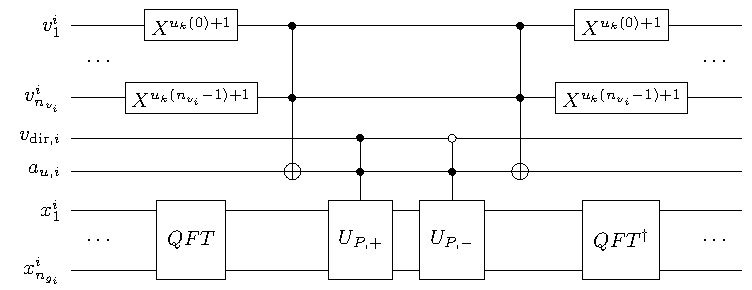
\includegraphics{imgs/cqlbm/streaming ancilla.pdf}
% \[
% \Qcircuit @C=1.3em @R=1em {
% %& & & & & \mbox{Rigetti generated amplitude amplification circuit} & & & & & \\
% \lstick{v^i_1} & \qw & \gate{X^{u_{k}(0)+1}} & \ctrl{4}  &\qw & \qw & \ctrl{4} & \gate{X^{u_{k}(0)+1}} & \qw & \qw\\
% \lstick{} & \cdots & & & & & & & \cdots & \\
% \lstick{v^i_{n_{v_i}}} & \qw & \gate{X^{u_{k}(n_{v_i}-1)+1}} & \ctrl{2}   &\qw  & \qw & \ctrl{2} & \gate{X^{u_{k}(n_{v_i}-1)+1}} &\qw &\qw\\
% \lstick{v_{\text{dir},i}} & \qw & \qw &  \qw & \ctrl{1} & \ctrlo{1} & \qw & \qw & \qw & \qw\\
% \lstick{a_{u,i}} & \qw & \qw & \targ  & \ctrl{1} & \ctrl{1} & \targ & \qw & \qw & \qw \\
% \lstick{x^i_1} & \qw  & \multigate{2}{QFT}  & \qw & \multigate{2}{U_{P,+}} &\multigate{2}{U_{P,-}} &\qw & \multigate{2}{QFT^\dagger} & \qw & \qw\\
% \lstick{} & \cdots &  & &  & & & & \cdots &  \\
% \lstick{x^i_{n_{g_i}}} & \qw & \ghost{QFT}   & \qw & \ghost{U_{P,+}} &\ghost{U_{P,-}} & \qw & \ghost{QFT^\dagger} & \qw & \qw\\
% }\] 
    \caption{Circuit representation of the proposed streaming step in dimension $i$ for one speed $|u_k|$ with ancilla qubit. Note that here we reset the $a_{u,i}$ ancilla after the streaming step. In the proposed algorithm this ancilla will only be reset after the reflection operation has been performed. }
    \label{fig:streaming_anc}
\end{figure}

\begin{figure}
    \centering
    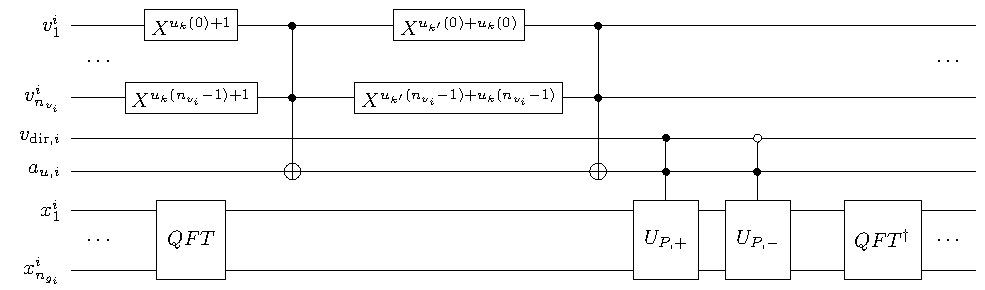
\includegraphics[scale = .75]{imgs/cqlbm/streaming k and k prime.pdf}
% \[
% \Qcircuit @C=1.3em @R=1em {
% %& & & & & \mbox{Rigetti generated amplitude amplification circuit} & & & & & \\
% \lstick{v^i_1} & \qw & \gate{X^{u_{k}(0)+1}} & \ctrl{4} &\qw & \gate{X^{u_{k+1}(0)+u_{k}(0)}} & \ctrl{4}  &\qw & \qw & \qw & \qw& \qw & \qw\\
% \lstick{} & \cdots & & & & & & & & & & \cdots & \\
% \lstick{v^i_{n_{v_i}}} & \qw & \gate{X^{u_{k}(n_{v_i}-1)+1}} & \ctrl{2} & \qw & \gate{X^{u_{k+1}(n_{v_i}-1)+u_{k}(n_{v_i}-1)}} & \ctrl{2}   &\qw  & \qw & \qw & \qw &\qw &\qw\\
% \lstick{v_{\text{dir},i}} & \qw & \qw &  \qw & \qw & \qw &  \qw & \ctrl{1} & \ctrlo{1} & \qw & \qw & \qw & \qw\\
% \lstick{a_{u,i}} & \qw & \qw & \targ & \qw & \qw & \targ  & \ctrl{1} & \ctrl{1} & \qw & \qw & \qw & \qw \\
% \lstick{x^i_1} & \qw  & \multigate{2}{QFT} & \qw & \qw & \qw  & \qw & \multigate{2}{U_{P,+}} &\multigate{2}{U_{P,-}} &\qw & \multigate{2}{QFT^\dagger} & \qw & \qw\\
% \lstick{} & \cdots &  & & &  & &  & & & & \cdots &  \\
% \lstick{x^i_{n_{g_i}}} & \qw & \ghost{QFT} & \qw & \qw & \qw  & \qw & \ghost{U_{P,+}} &\ghost{U_{P,-}} & \qw & \ghost{QFT^\dagger} & \qw & \qw\\
% }\] 
    \caption{Circuit representation of the proposed streaming step in dimension $i$ for two speeds $|u_k|$ and $|u_{k^\prime}|$ with ancilla qubit. Note how the proposed ancilla qubit allows to perform the streaming $U_{P,+}$ for both speeds in one operation. Here we do not reset the ancilla qubit $a_{u,i}$ after the streaming step, as in the proposed algorithm this ancilla will only be reset after the reflection operation has been performed.}
    \label{fig:streaming_anc two}
\end{figure}

% \begin{figure}
%     \centering
% \[
% \Qcircuit @C=1.3em @R=1em {
% %& & & & & \mbox{Rigetti generated amplitude amplification circuit} & & & & & \\
% \lstick{v_0} & \qw & \gate{X^{u^j_0+1}} & \ctrl{4} &\qw & \gate{X^{u^{j+1}_0+1}} & \ctrl{4}  &\qw & \qw & \ctrl{4} & \gate{X^{u^j_0+1}} & \qw & \qw\\
% \lstick{} & \cdots & & && & & & & & & \cdots & \\
% \lstick{v_m} & \qw & \gate{X^{u^j_m+1}} & \ctrl{2} & \qw & \gate{X^{u^{j+1}_m+1}} & \ctrl{2}   &\qw  & \qw & \ctrl{2} & \gate{X^{u^j_m+1}} &\qw &\qw\\
% \lstick{v_\text{dir}} & \qw & \qw &  \qw & \qw & \qw &  \qw & \ctrl{1} & \ctrlo{1} & \qw & \qw & \qw & \qw\\
% \lstick{a_{u,i}} & \qw & \qw & \targ & \qw & \qw & \targ  & \ctrl{1} & \ctrl{1} & \targ & \qw & \qw & \qw \\
% \lstick{x_0} & \qw  & \multigate{2}{QFT} & \qw & \qw & \qw  & \qw & \multigate{2}{U_{P,+}} &\multigate{2}{U_{P,-}} &\qw & \multigate{2}{QFT^\dagger} & \qw & \qw\\
% \stick{} & \cdots &  & & &  & &  & & & & \cdots &  \\
% \lstick{x_m} & \qw & \ghost{QFT} & \qw & \qw & \qw  & \qw & \ghost{U_{P,+}} &\ghost{U_{P,-}} & \qw & \ghost{QFT^\dagger} & \qw & \qw\\
% }\] 
%     \caption{Circuit representation of the proposed streaming step for one speed $|u_j|$ with ancilla qubit. If there are multiple speeds $|u_j|$ for which the particles traveling at that speed reach the next grid point in the timestep, we simply also flip the ancilla qubit $a_{u,i}$ for those speeds before performing the controlled $U_{P,+}$ and $U_{P,-}$ operations.}
%     \label{fig:streaming_anc}
% \end{figure}


Let ${u_{k}(n)}$ represent the value of the $n$-th bit when representing the index of the speed $u_{k}$ in the velocity vector\footnote{For example, assume we want to control on the speed being equal to $u_2$, let $\ket{u_2} = \ket{v_\text{dir}v_m \dots v_0} = \ket{10010}$. Then ${u_{2}(0)} = 0$ and ${u_{2}(1)} = 1$ etc. }. Then, we perform the operation $X^{u_k(l-1)+1}$ on each qubit $v^i_l \in \{v^i_{1}, \dots, v^i_{n_{v_i}}\}$ followed by the multi-controlled NOT operation between the $v^i_{1} \dots v^i_{n_{v_i}}$ qubits and the $a_{u,i}$ qubit for all speeds $|u_k|$ that take a step in the given time step, before performing the controlled streaming operations. Notice that we need to make sure to apply the $X^{u_k(l-1)+1}$ operations again after performing the multi-controlled NOT, to reset the speeds to their original states before we apply the $X^{u_{k^\prime}(l-1)+1}$ associated with the next speed $u_{k^\prime}$ for which the particles need to be streamed in this timestep. Furthermore, notice that we can simply combine these subsequent operations and get $X^{u_k(l-1)+1+u_{k^\prime}(l-1)+1} = X^{u_k(l-1)+u_{k^\prime}(l-1)}$ to be applied before the multi-controlled NOT operation to set the ancilla $a_{u,i}$ for the speed $u_{k^\prime}$. Figure \ref{fig:streaming_no_anc} shows the circuit of the streaming step without the ancilla $a_{u,i}$. Figure \ref{fig:streaming_anc} shows what the circuit of the streaming step with the ancilla $a_{u,i}$ looks like when streaming the particles with speed $u_k$ in dimension $i$. Figure \ref{fig:streaming_anc two} shows how using the ancilla qubit $a_{u,i}$ enables streaming the particles with several (in this example two) speeds $u_k$ and $u_{k^\prime}$ in dimension $i$ using a single $U_{p,+}$ and $U_{p,-}$ operation. In Figure \ref{fig:streaming_anc two} we do not reset the ancilla qubit $a_{u,i}$ after performing the streaming step, as in practice these will only get reset after the specular reflection step of the algorithm has been performed. 

In the above we have presented the streaming algorithm for a single dimension $i$. When working with multiple dimensions we perform the exact same operations in each dimension. Note how the streaming of the particle in the different dimensions can be applied to the qubits simultaneously, as different qubits are involved in the streaming step for each dimension. 
% Furthermore, we will make use of the state of these ancilla qubits $a_{u,i}$ in the specular reflection step of the algorithm, exploiting that now we can use these states in this step ``for free''. This means that in practice we do not reset the ancilla qubits $a_{u,i}$ after the specular reflection step, but we wait with doing this until after the specular reflection step has been completed. In Figure \ref{fig:streaming_anc two} we present how the streaming method with ancilla qubit can be used to stream particles of several (in this case two) speeds $u_j, u_{j+1}$ at the same time. In this Figure we also show what the streaming step implemented in the algorithm will look like, since we do not reset the ancilla qubit $a_{u,i}$ as in practice those will only be reset after the reflection step has been performed.
% % See Figure \ref{} for the exact quantum building block that is applied to the qubits in the quantum algorithm in the streaming step.\\
% In Figures \ref{fig:streaming_no_anc} and \ref{fig:streaming_anc} we give a circuit representation of our proposed streaming algorithm (including cancellation of interior QFT$^\dagger$ QFT pairs) both with and without the extra ancilla qubit when streaming the particles of only one speed $u_j$. In Figure \ref{fig:streaming_anc two} we present how the streaming method with ancilla qubit can be used when particles of multiple (in this case two) speeds $u_j, u_{j+1}$ are streamed at the same time. In this Figure we also show what the streaming step implemented in the algorithm will look like, since we do not reset the ancilla qubit $a_{u,i}$ as in practice those will only be reset after the reflection step has been performed.
% % @MEREL make this picture, misschien ook in the quantum overview total blahblah hoofdstuk?


% \subsection{CFL counter}\label{ssec:cfl_counter implemented}

% Now that we have described quantum circuits that implement a streaming step for particles of a specific velocity in each time step, we must also explain how to use these quantum circuits as blocks to build up the total algorithm. 

% In each time step $m$ of the algorithm we need to make sure that the particles with the right velocities are incremented (decremented) one step in space. We do this by letting the streaming step of the algorithm be built up of quantum circuits as described in Section \ref{ssec:convection step} for the speeds $u \in \mathcal{U}$ reaching the next grid point. In order for quantum algorithm to be efficiently implementable for variable velocity vectors, we need to describe an algorithm to build up our total algorithm using these quantum blocks. 

% We do this by making use of the CFL counter as described in Section \ref{ssec:cfl_counter}. Specifically, we first calculate the values $\Delta t_m$ as described in Equation \eqref{eq:delta_t} on a classical computer before creating the quantum circuit. When calculating the values $\Delta t_m$, we simultaneously keep track of which velocities reach the next grid point in each time step. This list is finally used to build up the correct quantum circuit, where in each time step the right particles get streamed to the next grid point. 

% To do this we use the following algorithm:  
% \begin{minted}{python}
% def time_series(Nv, M):
%     steps = 0
%     C = np.zeros(int(Nv/2))
%     v_p = np.arange(.5, Nv/2+ .5, 1)
%     recip = np.reciprocal(v_p)
%     ones = np.ones(int(Nv/2))
%     speed_ctrl = []
%     for i in range(M):
%         mult = np.multiply(ones - C,recip)
%         argmin = np.argmin(mult)
%         mini = mult[argmin]
%         C = C + mini*v_p
%         vels = []
%         for i in range(Nv/2): 
%             if round(C[i],6)== 1:
%                 C[i]=0
%                 vels.append(i)
%         C[argmin] = 0
%         speed_ctrl.append(vels)
%         steps+=1
%         if np.count_nonzero(np.round(C,6)==0.) + np.count_nonzero(np.round(C,6) == 1.) == int(Nv/2):
%             break
%     return speed_ctrl
% \end{minted}

% Clearly in this implementation we need $M N_v$ steps to create the time series, where $M$ is a pre-determined hyperparameter. So the complexity of this calculation is linear. In \cite{Todorova2020} they show that the value of $M$ is observed to grow linearly in $N_v$ with a factor 4, leading to the approximation 
% \begin{equation}
%     M \approx 4 N_v,
% \end{equation}
% so the complexity of calculating the right incrementation step is estimated to be quadratic in $N_v$. And in practice can be done quickly and efficiently on a classical computer. 



% \subsubsection{Multi-dimensional case}
% The general extension to the multi-dimensional case is trivial. Note that since we encode the velocities of the different dimensions in the same qubits, using extra qubits to keep track of the dimensions, we can exploit this in the case that the velocities are the same in each dimension.


% \[
% \Qcircuit @C=1.3em @R=1em {
% %& & & & & \mbox{Rigetti generated amplitude amplification circuit} & & & & & \\
% \lstick{v_0} & \qw & \gate{X^{v^i_0}} & \ctrl{5} &\qw & \qw & \ctrl{5} & \gate{X^{v^i_0}} & \qw & \qw\\
% \lstick{} & \cdots & & & & & & & \cdots & \\
% \lstick{v_m} & \qw & \gate{X^{v^i_m}} & \ctrl{3} &\qw & \qw & \ctrl{3} & \gate{X^{v^i_0}} &\qw &\qw\\
% \lstick{v_{dir}} & \qw & \qw & \qw & \ctrl{2} & \ctrlo{2} & \qw & \qw & \qw & \qw\\
% \lstick{v_{dim}} & \qw & \qw & \qw & \qw & \qw & \qw & \qw & \qw & \qw\\
% \lstick{a_{u,i}} & \qw & \qw & \targ & \ctrl{1} & \ctrl{1} & \targ & \qw & \qw & \qw \\
% \lstick{x_0} & \qw & \qw & \qw & \multigate{2}{incr} &\multigate{2}{decr} &\qw & \qw & \qw & \qw\\
% \stick{} & \cdots & & &  & & & & \cdots &  \\
% \lstick{x_m} & \qw & \qw & \qw & \ghost{incr} &\ghost{decr} & \qw & \qw & \qw & \qw\\
% \lstick{y_0} & \qw & \qw & \qw & \multigate{2}{incr} &\multigate{2}{decr} &\qw & \qw & \qw & \qw\\
% \stick{} & \cdots & & &  & & & & \cdots &  \\
% \lstick{y_m} & \qw & \qw & \qw & \ghost{incr} &\ghost{decr} & \qw & \qw & \qw & \qw\\
% }\] 





\subsection{Quantum specular reflection step}\label{sec:complete quantum specular reflection step}
After the completion of the streaming operation particles that come into contact with an obstacle and have virtually moved into it have to change their travel path; See Section \ref{ssec:class_reflection}. 

\normalem
Here, we propose a novel and fail-safe approach to the quantum reflection operation. 
First, the particles that virtually traveled into the obstacle have their velocity direction reversed in the direction normal to the wall encountered. 
Afterwards, these particles are placed back into the flow domain. As a result of both operations, the particle is located in the correct grid point and travels in the right physical direction in the next time step.
% In order to achieve this we need to carefully analyze the different cases possible for particle-wall interaction and find a unitary method that portrays the correct behavior in all separate cases. 

To achieve this there are some corner cases that need to be taken into account explicitly to avoid incorrect reflections, furthermore we make sure that there are no particles residing inside the object at the end of a time step. 
% For readability we will define our method for the 2-dimensional case below and give the n-dimensional abstraction in the appendix. @MEREL zou wel vet zijn als ik het naar n-dimensies kan vertalen & bewijzen :D \\

% In order to show that our method leads to the correct result for all possible particle wall interaction we will consider two separate cases. In the first case we consider the interaction of a particle with a wall, in a grid point inside the wall that is not a corner point. In the second case we will consider the more interesting case, of when a particle hits the wall in a so-called corner point. 


\subsubsection{Specular reflection steps - requirements and possible breakdown cases}
% Section \ref{ssec:class_reflection} provides the overview of what is required to happen in the reflection step. In this section we will go over how these requirements translate into the quantum implementation, and which possible breakdown cases must be taken into account. Strategies to mitigate this erroneous behavior will be presented in Section \ref{ssec:Correct Reflection}.
In this section, we translate the general procedure of the reflection step into a concrete quantum algorithm. Strategies to mitigate the erroneous behavior that might occur for the different corner cases will be discussed on Section \ref{ssec:Correct Reflection}

First we need to identify particles that have reached a grid point inside the obstacle, to ensure that they are placed back into the fluid domain before the start of the next streaming step.
This means that controlled on the current location of the particles (namely inside the obstacle), we set them back onto a grid point outside of the obstacle. Performing such an operation on a quantum computer is, however, far from trivial since we cannot alter the state of certain qubits controlled on their own states, as this would constitute a non-unitary operation. 
In our case this means that we cannot simply alter the position of the particles in space based on their current position, as that would be precisely attempting an operation on some qubits controlled by themselves. 

A way to overcome this is to use a system of ancillae to facilitate this back placement. This, however, introduces a new complexity since the ancillae would also have to be reset after the positional move has been performed in order to be usable in the next time step.
The resetting of the ancillae to their original position is nontrivial because we clearly cannot use the original requirements to simply flip the ancillae back, as the original control states were positional and we used the ancillae to control a positional change. Instead, we will have to reset the ancillae based on the new location of the particles in combination with their direction and velocities, i.e., we reverse engineer the particles' previous position. 

Another nontrivial aspect of the specular reflection step is to implement it such that all of the reflections are physically correct and we do not encounter unphysical behavior around the corner points. 
If one were to simply reflect the velocity in the $y$-direction upon hitting a $y$-wall and the velocity in the $x$-direction upon hitting an $x$-wall, incorrect behavior around the corner points will emerge. This is because corner points are points inside the object that are part of walls in multiple directions, i.e., in the two-dimensional case they are part of both an $x$-wall and a $y$-wall. 
What will happen in a non-fail-safe implementation of the specular reflection step is that particles hitting such a grid point coming through just the $x$- or $y$-wall have their velocities reflected in both directions, instead of only the one orthogonal to the wall they came through. 

Figure \ref{fig:example_wrong} gives an example of what can go wrong in a non-fail-safe implementation of the specular reflection step.
We see that in the cases of the green arrows the behavior is correct, as the velocity is reflected in both the $x$- and $y$-direction since the particle hits both an $x$- and $y$-wall. For the case of the blue arrows we see that the behavior is also correct, since the velocity parallel to the wall is zero in this case, therefore reflecting the velocity in this direction has no effect. However, for any particle approaching the corner point from another direction, such as the red arrow, the reflection based on a non-fail-safe implementation will certainly be wrong.  This is due to the fact that such a particle hits a point associated to both an $x$-wall \emph{and} a $y$-wall, even though physically it can easily be seen that the particle only hits either an $x$- \emph{or} a $y$-wall. In a non-fail-safe reflection operation this means that the velocity of the particle is erroneously reversed in both the $x$- \emph{and} the $y$-direction. When considering the shape of the wall and the direction of the particle, it is clear that in these cases only one of the two velocity components should be flipped, namely the velocity component orthogonal to the wall that the particle hits. 
%This leads to the majority of the particles that hit a corner point getting reflected erroneously in a non-fail-safe implementation. 

% Finally we need to consider the possible erroneous behaviors that might occur when $c_\text{rel} >1$ as described in Section \ref{ssec:case2 refl}. Specifically we need to ensure a particle gets reflected when it hits a wall but never actually reaches a grid point inside the object and we need to ensure a particle gets reflected in the correct dimension when a corner point is hit in such cases. 

% Since we already have to make use of extra ancillae to facilitate moving the particles out of the material before the end of the time step, we can use these same ancillae to keep track of which velocity directions should be reflected when a particle hits the object in the corner points. This avoids the problem shown in Figure \ref{fig:example_wrong}, that occurs in the specular reflection step when we do not explicitly keep track of which velocities should be reflected.  
% This does mean that we can only reset the ancillae $a_{v,i}$ after the specular reflection step, and not directly after performing the streaming operation. \\


\begin{figure}
    \centering
    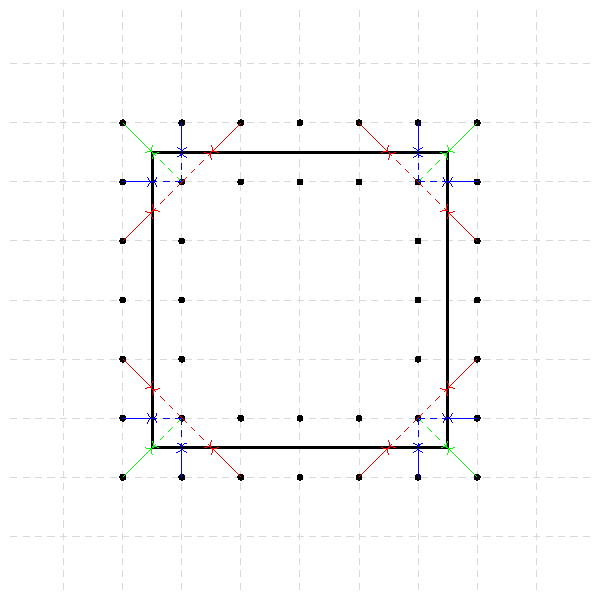
\includegraphics[]{imgs/cqlbm/wrong reflection example.pdf}
    % \begin{tikzpicture}
    % \draw[help lines, color=gray!30, dashed] (-4.9,-4.9) grid (4.9,4.9);
    % \draw[-,color=black] (-2.5,-2.5) -- (-2.5,2.5);
    % \draw[-,color=black] (-2.5,-2.5) -- (2.5,-2.5);
    % \draw[-,color=black] (2.5,-2.5) -- (2.5,2.5);
    % \draw[-,color=black] (-2.5,2.5) -- (2.5,2.5);
    % \foreach \j in {0,...,6}
    % {
    %     \foreach \i in {0,1}
    %     {
    %         \node at (-3+\i,-3+\j)[circle, fill, color = black, inner sep=1pt]{};
    %         \node at (2+\i,-3+\j)[circle, fill, color = black, inner sep=1pt]{};
    %     }
    % }
    % \foreach \j in {0,1}
    % {
    %     \foreach \i in {0,...,4}
    %     {
    %         \node at (-1+\i,-3+\j)[circle, fill, color = black, inner sep=1pt]{};
    %         \node at (-1+\i,2+\j)[circle, fill, color = black, inner sep=1pt]{};
    %     }
    % }


    % \foreach \i in {0,1}
    % {
    %     \draw[->, color=green] (-6*\i+3,-6*\i+3) -- (-5*\i+2.5,-5*\i+2.5);
    %     \draw[->, color=green] (6*\i-3,-6*\i+3) -- (5*\i-2.5,-5*\i+2.5);
        
    %     \draw[->, dashed, color=green] (2-4*\i,2-4*\i) --  (-5*\i+2.5,-5*\i+2.5);
    %     \draw[->, dashed, color=green] (-2+4*\i,2-4*\i) -- (5*\i-2.5,-5*\i+2.5);
        
        
        
    %     \draw[->, dashed, color=blue] (2,2) --  (2.5-.5*\i,2+.5*\i);
    %     \draw[->, color=blue] (3-1*\i,2+\i) -- (2.5-.5*\i,2+.5*\i) ;
    %     %\draw[->, color=blue] (2,2) --  (2+1*\i,3-\i);
        
    %     \draw[->, dashed, color=blue] (-2,2) --  (-2-.5*\i,2.5-.5*\i);
    %     \draw[->, color=blue] (-2-1*\i,3-\i) --  (-2-.5*\i,2.5-.5*\i);
        
    %     \draw[->, dashed, color=blue] (-2,-2) --  (-2-.5*\i,-2.5+.5*\i);
    %     \draw[->, color=blue] (-2-1*\i,-3+\i) --  (-2-.5*\i,-2.5+.5*\i);
        
    %     \draw[->, dashed, color=blue] (2,-2) --  (2+.5*\i,-2.5+.5*\i);
    %     \draw[->, color=blue] (2+\i,-3+\i) -- (2+.5*\i,-2.5+.5*\i);
        
    %     %\draw[->, color=red] (2,2) --  (3-2*\i,1+2*\i);
    %     \draw[->, dashed, color=red] (2,2) --  (2.5 -\i,1.5+\i);
    %     \draw[->,  color=red] (3 -2*\i,1+2*\i) --  (2.5 -\i,1.5+\i);
        
        
    %     \draw[->, dashed, color=red] (-2,2) --  (-2.5+\i,1.5+\i);
    %     \draw[->, color=red] (-3+2*\i,1+2*\i) -- (-2.5+\i,1.5+\i);
        
    %     \draw[->, dashed, color=red] (-2,-2) --  (-2.5+\i,-1.5-\i);
    %     \draw[->, color=red] (-3+2*\i,-1-2*\i) --  (-2.5+\i,-1.5-\i);
        
    %     \draw[->, dashed, color=red] (2,-2) --  (2.5-\i,-1.5-\i);
    %     \draw[->, color=red] (3-2*\i,-1-2*\i) --  (2.5-\i,-1.5-\i);
    % }
    % \end{tikzpicture}
    \caption{Illustration of the different cases of specular reflection at the corner points of an obstacle. While particles traveling into the obstacle along the blue and green velocity trajectories are reflected correctly even by non-fail-safe reflection algorithms, particles approaching the corner points along the red-arrow trajectories require special treatment as is done in our fail-safe specular reflection algorithm.
 }
    
    \label{fig:example_wrong}
\end{figure}



% \begin{figure}[h]
%     \centering
%     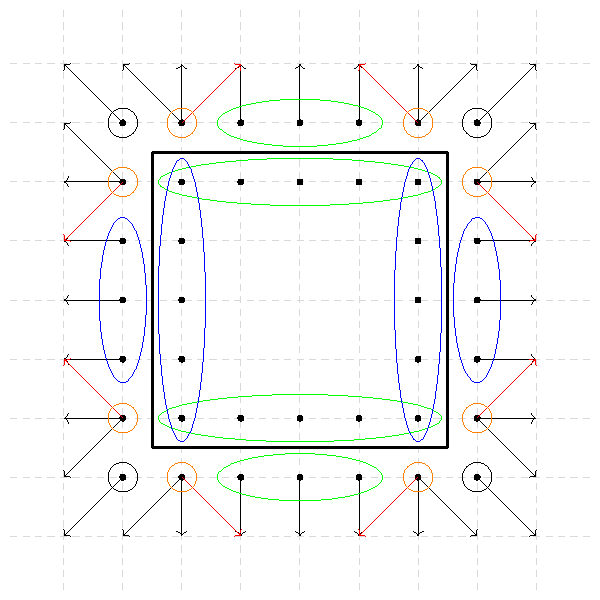
\includegraphics[width=.5\textwidth]{imgs/cqlbm/correct reflections.pdf}
%     % \begin{tikzpicture}
%     % \draw[help lines, color=gray!30, dashed] (-4.9,-4.9) grid (4.9,4.9);
%     % \draw[-,color=black] (-2.5,-2.5) -- (-2.5,2.5);
%     % \draw[-,color=black] (-2.5,-2.5) -- (2.5,-2.5);
%     % \draw[-,color=black] (2.5,-2.5) -- (2.5,2.5);
%     % \draw[-,color=black] (-2.5,2.5) -- (2.5,2.5);
%     % \foreach \j in {0,...,6}
%     % {
%     %     \foreach \i in {0,1}
%     %     {
%     %         \node at (-3+\i,-3+\j)[circle, fill, color = black, inner sep=1pt]{};
%     %         \node at (2+\i,-3+\j)[circle, fill, color = black, inner sep=1pt]{};
%     %     }
%     % }
%     % \foreach \j in {0,1}
%     % {
%     %     \foreach \i in {0,...,4}
%     %     {
%     %         \node at (-1+\i,-3+\j)[circle, fill, color = black, inner sep=1pt]{};
%     %         \node at (-1+\i,2+\j)[circle, fill, color = black, inner sep=1pt]{};
%     %     }
%     % }

%     % \foreach \i in {0,...,4}
%     % {
%     %     \draw[->] (-3,-2+\i) -- (-4,-2+\i);
%     %     \draw[->] (3,-2+\i) -- (4,-2+\i);
%     %     \draw[->, color = black] (-2+\i,-3) -- (-2+\i,-4);
%     %     \draw[->, color = black] (-2+\i,3) -- (-2+\i,4);
%     % }

    
%     % \foreach \i in {0,...,1}
%     % {
%     %     \draw[->, color=black] (-3,3-\i) -- (-4,4-\i);
%     %     \draw[->, color=black] (-3+\i,3) -- (-4+\i,4);
        
%     %     \draw[->, color=black] (-3,-3+\i) -- (-4,-4+\i);
%     %     \draw[->, color=black] (-3+\i,-3) -- (-4+\i,-4);
        
%     %     \draw[->, color=black] (3,-3+\i) -- (4,-4+\i);
%     %     \draw[->, color=black] (3-\i,-3) -- (4-\i,-4);
        
%     %     \draw[->, color=black] (3,3-\i) -- (4,4-\i);
%     %     \draw[->, color=black] (3-\i,3) -- (4-\i,4);
%     % }
    
    
%     % {
%     %     \draw[->, color=red] (-2,3) -- (-1,4);
%     %     \draw[->, color=red]  (-3,2) -- (-4,1);
        
%     %     \draw[->, color=red] (2,-3) -- (1,-4);
%     %     \draw[->, color=red] (3,-2) -- (4,-1);
        
%     %     \draw[->, color=red] (-2,-3) -- (-1,-4);
%     %     \draw[->, color=red] (-3,-2) -- (-4,-1);
        
%     %     \draw[->, color=red] (2,3) -- (1,4);
%     %     \draw[->, color=red] (3,2) -- (4,1);
%     % }

%     % \foreach \i in {0,...,1}
%     % {
%     %     \draw[color = black] (3-6*\i,3-6*\i) ellipse (.25cm and .25cm);
%     %     \draw[color = black] (-3+6*\i,3-6*\i) ellipse (.25cm and .25cm);
%     % }
    
%     % \foreach \i in {0,...,1}
%     % {
%     %     \draw[color = orange] (2-4*\i,3-6*\i) ellipse (.25cm and .25cm);
%     %     \draw[color = orange] (-3+6*\i,2-4*\i) ellipse (.25cm and .25cm);
%     % }
    
%     % \foreach \i in {0,...,1}
%     % {
%     %     \draw[color = orange] (2-4*\i,-3+6*\i) ellipse (.25cm and .25cm);
%     %     \draw[color = orange] (-3+6*\i,-2+4*\i) ellipse (.25cm and .25cm);
%     % }
    
    % \draw[color = green] (0,2) ellipse (2.4cm and .4cm);
%     % \draw[color = green] (0,-2) ellipse (2.4cm and .4cm);
%     % \draw[color = green] (0,3) ellipse (1.4cm and .4cm);
%     % \draw[color = green] (0,-3) ellipse (1.4cm and .4cm);
    
%     % \draw[color = blue] (2,0) ellipse (.4cm and 2.4cm);
%     % \draw[color = blue] (-2,0) ellipse (.4cm and 2.4cm);
%     % \draw[color = blue] (3,0) ellipse (.4cm and 1.4cm);
%     % \draw[color = blue] (-3,0) ellipse (.4cm and 1.4cm);
    
%     % \end{tikzpicture}
%     \caption{Illustration of all possible corner cases to be taken into account when particles collide with an obstacle (black box) and the physically correct reflection behavior as enforced by our fail-safe specular reflection algorithm.}
%     \label{fig:example_right}
% \end{figure}

\subsubsection{Fail-safe specular reflection - 2D case}\label{ssec:Correct Reflection}
In what follows we propose a novel fail-safe specular reflection approach. 
%In this section we develop a unitary operation that realizes fail-safe specular reflection in the two-dimensional case and we show how to practically implement this as a quantum algorithm. 
Figure \ref{fig:example_right} shows an obstacle placed on a grid, with both the grid points inside the object and the grid points outside the object drawn. Furthermore, Figure \ref{fig:example_right} shows the possible reflections that can occur around the obstacle. Using this figure we describe how we can implement a unitary operation that treats all possible reflection cases correctly. 
% First of all we define two extra sets of ancillae. We start by defining $d(d-1)$ extra ancillae $a_{c,i,j}$ that keep track of whether the absolute value of the speed is larger in dimension $i$ or dimension $j$. To make this more precise, we set $a_{c,i,j} = 1$ if and only if the absolute value of the speed is larger in dimension $i$ than in dimension $j$. For each dimension $i$ we require the ancillae $a_{c,i,j}$ and $a_{c,j,i}$ for $j \neq i$, leading to a total of $d(d-1)$ ancillae. Since the absolute values of the speeds in the dimensions does not change during the course of the algorithm, we need to set the value of these ancillae only once, therefore we consider setting the $a_{c,i,j}$ ancillae part of the state preparation step; see Section \ref{sssec:stateprep}.

First of all we require $d$ extra ancillae $a_{o,i}$, where $i$ represents the spatial dimension, that facilitate moving the particles out of the obstacle for the next time step and keeping track of which velocity components should be reflected when a particle hits a corner point. Lastly, we make use of the earlier defined ancillae $a_{u,i}$ to correctly set and reset the $a_{o,i}$ ancillae at the beginning and end of the specular reflection step, respectively. Note that using the $a_{u,i}$ ancillae does not add to the complexity of the circuit since we can reuse their state from the streaming step, and we reset them after the specular reflection step instead of directly performing the reset after the streaming operation.

Upon reaching a blue (green) encircled grid point inside the object, the particle has hit an $x$-wall ($y$-wall).
When hitting a grid point that is part of the $x$-wall ($y$-wall) in the object, we flip the ancilla qubit $a_{o,y}$ ($a_{o,x}$) controlled on the $v_{\text{dir},y}$ and $a_{u,y}$ ($v_{\text{dir},x}$ and $a_{u,x}$) qubits. %This means that in total this operation is controlled on a subset of the $g_i$ qubits (for all dimensions $i$) as well as the $v_{\text{dir},y}$ and $a_{u,y}$ ($v_{\text{dir},x}$ and $a_{u,x}$) qubits.

Specifically, we flip the extra-defined ancillae only when we just took a step in the direction that the wall reflects, and when we travel in a direction that the wall would reflect based on the position of the object (meaning that if we travel in the negative $y$-direction and we hit a grid point in a $y$-wall in the bottom of the object we do not flip the $a_{o,y}$ ancilla).
This is followed by flipping $v_{\text{dir},y}$ ($v_{\text{dir},x}$) controlled by the $a_{o,y}$ ($a_{o,x}$) ancillae and incrementing the position by one index in the $y$ ($x$) direction. Here, the term incrementing amounts to streaming in the direction $v_{\text{dir},y}$ ($v_{\text{dir},x}$).

% Now there are some cases for which the $a_{o,x}$ ($a_{o,y}$) ancilla are flipped wrongly. This happens when a particle reaches a corner point inside the object, i.e., a grid point that is associated with both an $x$- and $y$-wall, streamed from a black-encircled point outside of the object when $|u_x|\neq |u_y|$. In this case both the $a_{o,x}$ and $a_{o,y}$ ancillae will be set to one, when the particle in reality only hits either an $x$- or a $y$-wall. Figure \ref{} illustrates this with an example. 
% We will use this example to explain how we can correctly reset the $a_{o,x}$ or $a_{o,y}$ ancilla in such a case.
% In this case we nee
% @MEREL schrijf over resetten in het geval dat je in een hoekpunt komt op een manier die nu Ox en Oy zet, maar die eigenlijk maar een van beiden moet zetten. 


% @MEREL schrijf over the s corner cases that serve as a special wall. 

The final step consists of resetting the ancillae $a_{o,i}$. The grid points directly outside the object that are not `in the vicinity of a corner point' of the object constitute the trivial case. By `in the vicinity of a corner point' we mean that the current grid point the particle is in, has as adjacent grid point inside the object a grid point that is part of both an $x$-wall and a $y$-wall. In Figure \ref{fig:example_right} the grid points that are not considered to be `in the vicinity of a corner point' are identified as the green (blue) encircled grid points outside of the object. All that needs to be done for them is to reset the $a_{o,y}$ ($a_{o,x}$) ancilla controlled on the position, the direction of the $y$ ($x$) velocity and $a_{u,y}$ ($a_{u,x}$). More specifically, we reset the ancilla for a particle in a grid point that is adjacent to an $x$-wall ($y$-wall) if and only if $a_{u,y}=1$ ($a_{u,x}=1$) and $v_{\text{dir},y}$ ($v_{\text{dir},x}$) points away from the wall. 

Around the corner points of the object we need to be more careful, however. This is due to the fact that the particles could have gotten there via multiple directions, in which case different ancillae would need to be reset. 

For the black encircled grid points we have that both the ancillae $a_{o,y}$ and $a_{o,x}$ need to be reset controlled on $v_{\text{dir},y}$, $v_{\text{dir},x}$, $a_{u,x}$ and $a_{u,y}$. Only when $a_{u,x} = a_{u,y} = 1$ holds and $v_{\text{dir},y}$ and $v_{\text{dir},x}$ are such that they both point away from the object, do $a_{o,y}$ and $a_{o,x}$ need to be reset.

For the orange encirled points we do the following. We first reset the ancillae based on the same criteria as the green (blue) encircled qubits. Subsequently, we note that the respective ancilla should not have been reset only in the case of the red arrow. Therefore, we simply re-reset the ancillae based on the criteria that reflect the case of the red arrows, consisting of position in combination with direction in both the $x$ and $y$ direction ($v_{\text{dir},x}$, $v_{\text{dir},y}$) and whether a step was taken in both directions in the former time step ($a_{u,x}$ and $a_{u,y}$). Specifically, for the arrow located on the highest row on the left, this would mean resetting the ancilla controlled on $v_{\text{dir},y}$ being positive, $v_{\text{dir},x}$ being positive, the position being the dot on the highest row second from the left and $a_{u,x}$ and $a_{u,y}$ both being activated.
This strategy for defining hang-crafted resetting patterns can easily be adapted to the remaining three corners.



% \subsection{Encoding of the object}
% In order to implement an efficient and easily implementable quantum collisionless Boltzmann method we also need to provide an automatic encoding of the location of the quantum object.
% A smart choice and encoding of the location of the object is important to ensure that the total complexity of the algorithm stays constant in $n_g$.
% The encoding of the location of the object is important for the total complexity of the algorithm, as it determines the amount of blocks necessary to describe one quantum wall. Here we will describe a nontrivial object placement, that leads to a linear amount of quantum blocks necessary to describe a wall. We have implemented this method in such a way that the user only needs to give the required sizes of the wall, and the object and the resulting quantum circuits are created automatically. 

% To get the best complexity, we need to choose the lengths of the walls of the objects to be a power of two in the dimensions they do not reflect in. Furthermore we set the objects in the grid in such a way that the lowest grid point inside of the objects in all dimensions is the $\ket{0}$ state. \\
% We will now give a formal definition of this set-up. Let the wall $l$ be a $j$-wall. Then the length of the wall $l$ in the dimension $i$ can be written as $s_{l,i}=2^{n_{l,i}}$. Here $s_{l,i}$ are the total amount of grid points inside the object directly adjacent to the wall $l$ in the direction $i$.
% This means that in order to encode the flipping of the $a_{o,j}$ qubits based on the particles reaching a grid point inside the $j$-wall, we only need one set of multi-controlled NOT gates. This is due to the fact that for a $j$-wall $l$ of lengths $s_{l,i}$, we have that the location of the wall is encoded as ranging from: 
% \begin{equation}
%     \ket{\underbrace{0\dots 0}_{n_{g_i} - n_{l,i}} \overbrace{0 \dots 0}^{n_{l,i}}},
% \end{equation}
% to 
% \begin{equation}
%     \ket{\underbrace{0\dots 0}_{n_{g_i} - n_{l,i}} \overbrace{1 \dots 1}^{n_{l,i}}}.
% \end{equation}
% So we encode this by simply controlling on the first $n_{g_i}-n_{l,i}$ qubits to be in the $0$ state for all dimensions $i$ at the same time, while all other qubits encoding the position in the dimension $i$ can be in any combination of basis states and so we do not need to control on those. Notice that for a $j$-wall $l$ we have that $s_{l,j} = 1$ and so $n_{l,j}=0$. 
 
% Then for each $j$-wall we also need to encode the grid points directly outside of the object. This is necessary for the step where we reset the ancillae $a_{o,j}$ to ensure their usability in the next time step.
% In order to reset the $a_{o,j}$ qubits we need to control on the particles being in the position right next to the $j$-wall $l$. We can see the grid points constituting this region as its own $j$-wall of size $s^\prime_{l,i} = s_{i,l} + 2$ for each $i \neq j$. For the dimension $j$ this region will again have size $s^\prime_{l,j} = 1$.
% For the other dimensions $i \neq j$ the positions to control over are again ranging from the:
% \begin{equation}
%     \ket{\underbrace{0\dots 0}_{n_{g_j} - n_j} \overbrace{0 \dots 0}^{n_j}},
% \end{equation}
% to the
% \begin{equation}
%     \ket{\underbrace{0\dots 0}_{n_{g_j} - n_j} \overbrace{1 \dots 1}^{n_j}}
% \end{equation}
% state. Only now we need to add the $\ket{1\dots 1}$ and the $\ket{0\dots 1 0 \dots 0}$ states to control over in the dimension $j$. In this case we need to add 3 separate steps of at most $n$ control qubits per dimension $j$. We need to combine all the 3 separate state encodings for all the dimensions that are not $j$, so in total there are $3(d-1)$ separate multi-controlled NOT operations necessary to set back the ancillae $a_{o,j}$ for each wall $l$. This is the most expensive part of the specular reflection step, so in total the complexity will be $\mathcal{O}\left ( |W|d \right )$ where $|W|$ is the number of walls in the object.  

% So in total using this encoding we get that we require  $\mathcal{O}\left ( |W| d \right )$ multi-controlled NOT operations. 



\subsubsection{Fail-safe specular reflection - 3D case}\label{ssec:spec ref 3d}
We will now provide a generalization of our two-dimensional method to three dimensions. The idea of the set-up is the same, we define grid points just inside the object and grid points outside and directly adjacent to the object. 
Then, each grid point inside the object is associated with an $xy$-wall or an $xz$-wall or a $yz$-wall.
Now, if a particle reaches a grid point associated to an $xy$-wall ($xz$-wall, $yz$-wall), was traveling in a direction that this wall would reflect (meaning $v_{\text{dir},z}$ ($v_{\text{dir},y}$, $v_{\text{dir},x}$) was in the right state) and $a_{u,z}=1$ ($a_{u,y}=1$, $a_{u,x}=1$), the ancilla $a_{o,z}$ ($a_{o,y}$, $a_{o,x}$) will be flipped. Notice that here we are using the exact same logic as in the two-dimensional case.

Subsequently the particles are placed back to the adjacent points inside the fluid domain based on the states of $a_{o,x}$, $a_{o,y}$ and $a_{o,z}$. This step is realized in the same way as in the two-dimensional case.

Finally, we need to reset the ancillae $a_{o,x}$, $a_{o,y}$ and $a_{o,z}$. This is again performed by considering the current position of the particle, in combination with their direction and whether or not they were streamed in the last time step. Compared to the two-dimensional case, in three dimensions there are more distinct cases to be taken into account. Instead of distinguishing only between corner points and non-corner points, we need to distinguish between corner points (where three walls come together), points along the edges of the obstacle (where two walls come together) and points on the side of the objects. 

For the points on the side of the object and the points along the edges of the obstacle, the rules for reflection will be the same as in the two-dimensional case. Here the points on the edges of the obstacle behave the same as the corner points in the two-dimensional case, and the points on the side of the objects behave the same as the non-corner points in the two-dimensional case. 

The corner points where three walls come together require a more in depth consideration. Figures \ref{fig:3dpict} and \ref{fig:3dpictin2d} show an object in our three-dimensional grid and uses colors to indicate which grid points need to be taken into account as special cases around corner points.
In the black encircled points the $a_{o,z}$, $a_{o,y}$ and $a_{o,x}$ qubits are reset if the velocity in all three dimensions travels away from the object and the ancillae $a_{u,x}$, $a_{u,y}$, $a_{u,z}$ are all equal to 1. 
In the red encircled points the ancillae of the two dimensions which get reflected by the two walls that intersect are reset, if the particle is moving away from the object in the two respective dimensions and the particle took a step in both dimensions and just before did not travel a step in the third dimension towards the object.
In the blue encircled point we consider the following behaviors. Here we only reset the ancilla associated with the dimension the wall reflects in if we just took a step in that dimension and the directional qubit points away from the object. Furthermore, we need to check that in none of the other two dimensions we just took a step towards the object. 

\begin{figure}[h]
\centering
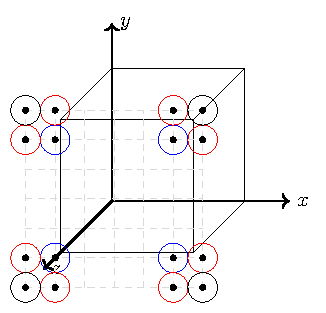
\includegraphics[]{imgs/cqlbm/special cases 3D.pdf}
% \begin{tikzpicture} 
% 		[cube/.style={black},
% 			grid/.style={thin, dashed,color=gray!30},
% 			axis/.style={->,black, thick}]

% 	%draw a grid in the x-y plane

% 	%draw the axes
% 	\draw[axis] (0,0,0) -- (3,0,0) node[anchor=west]{$x$};
% 	\draw[axis] (0,0,0) -- (0,3,0) node[anchor=west]{$y$};
% 	\draw[axis] (0,0,0) -- (0,0,3) node[anchor=west]{$z$};
	
% 	%draw the top and bottom of the cube
% 	\draw[cube] (0,0,0) -- (0,2.25,0) -- (2.25,2.25,0) -- (2.25,0,0) -- cycle;
% 	\draw[cube] (0,0,2.25) -- (0,2.25,2.25) -- (2.25,2.25,2.25) -- (2.25,0,2.25) -- cycle;
	
% 	%draw the edges of the cube
% 	\draw[cube] (0,0,0) -- (0,0,2.25);
% 	\draw[cube] (0,2.25,0) -- (0,2.25,2.25);
% 	\draw[cube] (2.25,0,0) -- (2.25,0,2.25);
% 	\draw[cube] (2.25,2.25,0) -- (2.25,2.25,2.25);

% 	\foreach \x in {-.5,0,...,2.5}
% 		\foreach \y in {-.5,0,...,2.5}
% 		{
% 			\draw[grid] (\x,-.5,2.5 ) -- (\x,2.5,2.5);
% 			\draw[grid] (-.5,\y,2.5) -- (2.5,\y,2.5 );
% 		}
		
% 	\draw[color=green] (2,2,2.5) ellipse (.25cm and .25cm);
%     \node at (2,2,2.5)[circle, fill, color = black, inner sep=1pt]{};
    
%     \draw[color=green] (0,2,2.5) ellipse (.25cm and .25cm);
%     \node at (0,2,2.5)[circle, fill, color = black, inner sep=1pt]{};
    
%     \draw[color=green] (2,0,2.5) ellipse (.25cm and .25cm);
%     \node at (2,0,2.5)[circle, fill, color = black, inner sep=1pt]{};
    
%     \draw[color=green] (0,0,2.5) ellipse (.25cm and .25cm);
%     \node at (0,0,2.5)[circle, fill, color = black, inner sep=1pt]{};
    
%     \draw[color=red] (2,2.5,2.5) ellipse (.25cm and .25cm);
%     \node at (2,2.5,2.5)[circle, fill, color = black, inner sep=1pt]{};
    
%     \draw[color=red] (0,2.5,2.5) ellipse (.25cm and .25cm);
%     \node at (0,2.5,2.5)[circle, fill, color = black, inner sep=1pt]{};
    
%     \draw[color=red] (2,-.5,2.5) ellipse (.25cm and .25cm);
%     \node at (2,-.5,2.5)[circle, fill, color = black, inner sep=1pt]{};
    
%     \draw[color=red] (0,-0.5,2.5) ellipse (.25cm and .25cm);
%     \node at (0,-.5,2.5)[circle, fill, color = black, inner sep=1pt]{};
    
    
%     \draw[color=red] (2.5,2,2.5) ellipse (.25cm and .25cm);
%     \node at (2.5,2,2.5)[circle, fill, color = black, inner sep=1pt]{};
    
%     \draw[color=red] (-.5,2,2.5) ellipse (.25cm and .25cm);
%     \node at (-0.5,2,2.5)[circle, fill, color = black, inner sep=1pt]{};
    
%     \draw[color=red] (2.5,0,2.5) ellipse (.25cm and .25cm);
%     \node at (-.5,0,2.5)[circle, fill, color = black, inner sep=1pt]{};
    
%     \draw[color=red] (-.5,0,2.5) ellipse (.25cm and .25cm);
%     \node at (2.5,0,2.5)[circle, fill, color = black, inner sep=1pt]{};
    
%     \draw[color=black] (2.5,2.5,2.5) ellipse (.25cm and .25cm);
%     \node at (2.5,2.5,2.5)[circle, fill, color = black, inner sep=1pt]{};
    
%     \draw[color=black] (-0.5,2.5,2.5) ellipse (.25cm and .25cm);
%     \node at (-0.5,2.5,2.5)[circle, fill, color = black, inner sep=1pt]{};
    
%     \draw[color=black] (2.5,-0.5,2.5) ellipse (.25cm and .25cm);
%     \node at (2.5,-0.5,2.5)[circle, fill, color = black, inner sep=1pt]{};
    
%     \draw[color=black] (-.5,-0.5,2.5) ellipse (.25cm and .25cm);
%     \node at (-.5,-.5,2.5)[circle, fill, color = black, inner sep=1pt]{};
			
% % 	%draw the top and bottom of the cube
% % 	\draw[cube] (0.5,0.5,0.5) -- (0.5,2.5,.5) -- (2.5,2.5,0.5) -- (2.5,0.5,0.5) -- cycle;
% % 	\draw[cube] (0.5,0.5,2.5) -- (0.5,2.5,2.5) -- (2.5,2.5,2.5) -- (2.5,0.5,2.5) -- cycle;
	
% % 	%draw the edges of the cube
% % 	\draw[cube] (0.5,0.5,0.5) -- (0.5,0.5,2.5);
% % 	\draw[cube] (0.5,2.5,0.5) -- (0.5,2.5,2.5);
% % 	\draw[cube] (2.5,0.5,0.5) -- (2.5,0.5,2.5);
% % 	\draw[cube] (2.5,2.5,0.5) -- (2.5,2.5,2.5);
	
% \end{tikzpicture}
\caption{Illustration of the corner cases specific to a three-dimensional obstacle. The action applied to the different color-coded grid points is described in Section \ref{ssec:spec ref 3d}.}\label{fig:3dpict}
\end{figure}

\begin{figure}[h]
    \centering
    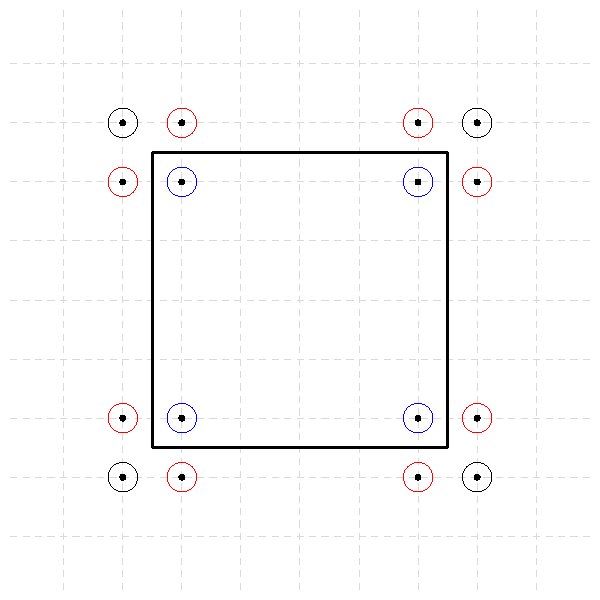
\includegraphics[]{imgs/cqlbm/special cases 3D 2.pdf}
    % \begin{tikzpicture}
    % \draw[help lines, color=gray!30, dashed] (-4.9,-4.9) grid (4.9,4.9);
    % \draw[-,color=black] (-2.5,-2.5) -- (-2.5,2.5);
    % \draw[-,color=black] (-2.5,-2.5) -- (2.5,-2.5);
    % \draw[-,color=black] (2.5,-2.5) -- (2.5,2.5);
    % \draw[-,color=black] (-2.5,2.5) -- (2.5,2.5);
    % \foreach \j in {0,1}
    % {
    %     \foreach \i in {0,1}
    %     {
    %         \node at (-3+\i,-3+\j)[circle, fill, color = black, inner sep=1pt]{};
    %         \node at (2+\i,-3+\j)[circle, fill, color = black, inner sep=1pt]{};
    %     }
    % }
    
    % \foreach \j in {5,6}
    % {
    %     \foreach \i in {0,1}
    %     {
    %         \node at (-3+\i,-3+\j)[circle, fill, color = black, inner sep=1pt]{};
    %         \node at (2+\i,-3+\j)[circle, fill, color = black, inner sep=1pt]{};
    %     }
    % }
    
    % \foreach \j in {0,1}
    % {
    %     \foreach \i in {0,...,4}
    %     {
    %      %   \node at (-1+\i,-3+\j)[circle, fill, color = black, inner sep=1pt]{};
    %      %  \node at (-1+\i,2+\j)[circle, fill, color = black, inner sep=1pt]{};
    %     }
    % }


    % \foreach \i in {0,1}
    % {
    %     \draw[color=black] (-6*\i+3,-6*\i+3) ellipse (.25cm and .25cm);
    %     \draw[color=black] (6*\i-3,-6*\i+3) ellipse (.25cm and .25cm);
        
    %   % \draw[->, dashed, color=green] (2-4*\i,2-4*\i) --  (-5*\i+2.5,-5*\i+2.5);
    %   % \draw[->, dashed, color=green] (-2+4*\i,2-4*\i) -- (5*\i-2.5,-5*\i+2.5);
        
        
        
    %     \draw[color=green] (2,2) ellipse (.25cm and .25cm);
    %     \draw[color=red] (3-1*\i,2+\i) ellipse (.25cm and .25cm) ;
    %     %\draw[->, color=blue] (2,2) --  (2+1*\i,3-\i);
        
    %     \draw[color=green] (-2,2) ellipse (.25cm and .25cm);
    %     \draw[color=red] (-2-1*\i,3-\i) ellipse (.25cm and .25cm);
        
    %     \draw[color=green] (-2,-2) ellipse (.25cm and .25cm);
    %     \draw[color=red] (-2-1*\i,-3+\i) ellipse (.25cm and .25cm);
        
    %     \draw[color=green] (2,-2) ellipse (.25cm and .25cm);
    %     \draw[color=red] (2+\i,-3+\i) ellipse (.25cm and .25cm);
        
    %     %\draw[->, color=red] (2,2) --  (3-2*\i,1+2*\i);
    %     % \draw[->, dashed, color=red] (2,2) --  (2.5 -\i,1.5+\i);
    %     % \draw[->,  color=red] (3 -2*\i,1+2*\i) --  (2.5 -\i,1.5+\i);
        
        
    %     % \draw[->, dashed, color=red] (-2,2) --  (-2.5+\i,1.5+\i);
    %     % \draw[->, color=red] (-3+2*\i,1+2*\i) -- (-2.5+\i,1.5+\i);
        
    %     % \draw[->, dashed, color=red] (-2,-2) --  (-2.5+\i,-1.5-\i);
    %     % \draw[->, color=red] (-3+2*\i,-1-2*\i) --  (-2.5+\i,-1.5-\i);
        
    %     % \draw[->, dashed, color=red] (2,-2) --  (2.5-\i,-1.5-\i);
    %     % \draw[->, color=red] (3-2*\i,-1-2*\i) --  (2.5-\i,-1.5-\i);
    % }
    % \end{tikzpicture}
    \caption{View from the positive $z$-axis onto the $xy$-wall of the obstacle. Note that the $xy$-wall lies half a grid point in the z-direction below the grid with the encircled points. 
 }\label{fig:3dpictin2d}
\end{figure}


% \begin{tikzpicture}[scale=3,tdplot_rotated_coords,
%                     cube/.style={very thick,black},
%                     grid/.style={very thin,gray},
%                     axis/.style={->,blue,ultra thick},
%                     rotated axis/.style={->,purple,ultra thick}]

%     %draw a grid in the x-y plane
%     \foreach \x in {-0.5,0,...,2.5}
%         \foreach \y in {-0.5,0,...,2.5}
%         {
%             \draw[grid] (\x,-0.5) -- (\x,2.5);
%             \draw[grid] (-0.5,\y) -- (2.5,\y);
%         }

%     %draw the main coordinate frame axes
%     \draw[axis,tdplot_main_coords] (0,0,0) -- (3.5,0,0) node[anchor=west]{$x$};
%     \draw[axis,tdplot_main_coords] (0,0,0) -- (0,3.5,0) node[anchor=north west]{$y$};
%     \draw[axis,tdplot_main_coords] (0,0,0) -- (0,0,3.5) node[anchor=west]{$z$};


%     %draw the rotated coordinate frame axes
%     % \draw[rotated axis] (0,0,0) -- (3,0,0) node[anchor=west]{$x'$};
%     % \draw[rotated axis] (0,0,0) -- (0,3,0) node[anchor=south west]{$y'$};
%     % \draw[rotated axis] (0,0,0) -- (0,0,3) node[anchor=west]{$z'$};

%     %draw the top and bottom of the cube
%     \draw[cube] (0,0,0) -- (0,2,0) -- (2,2,0) -- (2,0,0) -- cycle;

%     %draw the top and bottom of the cube
%     \draw[cube] (0,0,0) -- (0,2,0) -- (0,2,2) -- (0,0,2) -- cycle;

%     %draw the top and bottom of the cube
%     \draw[cube] (0,0,0) -- (2,0,0) -- (2,0,2) -- (0,0,2) -- cycle;

% \foreach \x in {0,1,2}
%   \foreach \y in {0,1,2}
%       \foreach \z in {0,1,2}{
%           %#####################################################
%           \ifthenelse{  \lengthtest{\x pt < 2pt}  }
%           {
%              % True
%                 \draw [black]   (\x,\y,\z) -- (\x+1,\y,\z);
%           }
%           {% False
%           }
%           %#####################################################
%           \ifthenelse{  \lengthtest{\y pt < 2pt}  }
%           {
%              % True
%                 \draw [black]   (\x,\y,\z) -- (\x,\y+1,\z);
%           }
%           {% False
%           }
%           %#####################################################
%           \ifthenelse{  \lengthtest{\z pt < 2pt}  }
%           {
%              % True
%                 \draw [black]   (\x,\y,\z) -- (\x,\y,\z+1);
%           }
%           {% False
%           }
%           %\shade[rotated axis,ball color = purple!80] (\x,\y,\z) circle (0.06cm);          
% }

% \end{tikzpicture}




\subsubsection{Efficient object encoding}
% In order to ensure polynomial complexity of our algorithm, we need to be able to determine whether or not a grid point is part of a given wall (or right outside the wall) in polynomial time. 
% This can be done trivially if we simply assume that the size of the walls grow, for instance, with a constant parameter of the amount of qubits used to encode the grid in a given dimension. This assumption, however, is highly restrictive. As this would imply that the amount of grid points grows exponentially with the amount of qubits (as it always does), but the wall size grows linearly. When adding more qubits to the system we then simply end up with a very small object in a very large space. And when assuming that the size of a wall grows linearly in the amount of grid points as is done in \cite{Todorova2020}, this assumption implies that the size of the wall grows exponentially in the amount of qubits required to encode the grid. Since we want to avoid exponential growth of the circuit in the number of qubits as well as an assumption leading to an unnatural restriction in object size, we propose a method that shows we can determine whether or not a grid is part of a wall in polynomial time for any given wall size. \\


In this section we propose a novel approach based on quantum comparison operations for encoding objects in a way that we can efficiently identify whether or not a grid point is part of a certain object wall. Our approach requires $2(d-1)$ extra ancillae and will be explained at the hand of a two-dimensional example.


% \xout{In this section we provide a novel quantum approach for encoding objects that can efficiently identify whether or not a grid point is part of a certain wall of an object.}

% \xout{We do this by making use of quantum comparison operations in combination with $2(d-1)$ extra ancillae. 
% We explain how to use this method via an example in the two-dimensional case.} \\

% \xout{In the two-dimensional case we use the quantum comparison method as follows. }
Assume that we want to encode a $y$-wall (note that everything works the same to encode an $x$-wall), for example the left-most $y$-wall of Figure \ref{fig:example_right}. Let the grid points just inside the object next to the $y$-wall, i.e., the left-most blue encircled grid points inside the object of Figure \ref{fig:example_right}, range from $[ a,b ]$ in the $y$-axis. We first need to determine whether or not we are in one of the left-most blue encircled grid points inside the object with the aid of two quantum comparison operations. The first quantum comparison operation checks whether $y \geq l$ holds. If so we flip the first extra ancilla from its start state $a_{a,1}= 0$ to $a_{a,1}= 1$. Then we check if $y \leq u$ holds, and if so we flip the second extra ancilla to $a_{b,1}= 1$. Now, controlled on these both ancillae and the state of the qubits encoding the position in the $x$ dimension of these left-most blue encircled qubits, we flip the ancilla $a_{o,x}$ indicating that we are in a wall which reflects the velocity in the $x$-direction.
Now we simply reset the $a_{a,1}$ and $a_{b,1}$ ancillae so that they can be reused for other walls, by performing the same quantum comparison operations as described before\footnote{Note that in the example of Figure \ref{fig:example_right} it would be most efficient to first flip the ancilla $a_{o,x}$ as well, controlled on the $a_{a,1}$ and $a_{b,1}$ qubits in combination with the qubits encoding the position in the $x$ dimension being in the position of the right-most blue encircled grid points inside the object. But for now we were only considering the left-most $y$-wall.}.
In the two-dimensional case we perform this operation for all walls in order to set the $a_{o,x}$ and $a_{o,y}$ qubits as required. After completion of this step we continue in the same fashion as described in Section \ref{ssec:Correct Reflection}.

What remains is to reset the $a_{o,x}$ and $a_{o,y}$ qubits after the reflection and streaming steps have been performed which we accomplish, again, with the aid of the quantum comparison operation. To continue with our example of the left-most $y$-wall of Figure \ref{fig:example_right}, we again perform two comparison operations to check whether we are in the left-most blue encircled grid points right outside the wall, which amounts to checking $y \in [l+1,u-1]$. This can be achieved with the same logic as before namely by checking $y \geq l+1$ and $y \leq u-1$. All the other steps and the resetting are performed in the same manner as explained before. The extension to the three-dimensional case is straightforward.






\subsubsection{Quantum Comparison Operation}\label{ssec: quantum comparison}
In our implementation we use the quantum comparison operation from \cite{Gidney2017}, which compares the integer value $i$ of the $n$-qubit quantum state $\ket{i}$ with a pre-determined constant $k$ saving the result of the comparison in a separate qubit. 

% The operation consists of one (periodic) subtraction operation defined on the total $n$+1 qubits followed by a (periodic) addition defined on the $n$ qubits encoding the original quantum state. Multiple realizations of quantum addition and subtraction operations are described in the literature \cite{Häner2017,Takahashi2009,Cuccaro2004,Draper1998}, all having their own complexities and required ancillae associated to them.

The quantum comparison algorithm works as follows. Say we wish to determine whether the integer value $i$ encoded in basis state $\ket{i}$ is smaller than $k$\footnote{Note that $k \leq 2^n-1$ always holds, since otherwise we trivially know that $k$ is larger than any value that $n$ qubits can encode.}. Then, we first subtract the integer $k$ from the value encoded by the $n+1$ qubits encoding the state $\ket{0}\otimes\ket{i}$, where the prepended $\ket{0}$ qubit will hold the result of the computation. Now there are two cases, $i\geq k$ and $i<k$. \\

Assume that we are in the case $i \geq k$. Then subtracting $k$ from $i$ encoded in  $\ket{0}\otimes\ket{i}$ gives $\ket{0}\otimes \ket{i-k}$, which leaves the prepended $\ket{0}$ qubit unchanged. 
Now we simply perform an addition of the value $k$ to the $n$-qubits that are used to encode $i$ and now encode $\ket{i-k}$. This gives $\ket{0}\otimes\ket{i-k+k} = \ket{i}$. And so in total we end up with a quantum register in the state $\ket{0}\otimes\ket{i}$. Where the $\ket{0}$ state is the result of the computation which means that $i \geq k$ in fact holds, and the last $n$ qubits are again in the original state $\ket{i}$. \\

Now let us assume that we are in the second case $i<k$. Again, we start by periodically subtracting the integer $k$ from $i$ encoded in the state $\ket{0}\otimes\ket{i}$, only now since $k>i$ we end up flipping the state of the prepended $\ket{0}$ qubit. This is because periodically subtracting $k$ from $i$ in a state encoded by $n+1$ qubits results in the state $\ket{2^{n+1} -1 - k +i}$. Since $k \leq 2^n-1$ and $i \geq 0$ we must have that $2^{n+1} -1 - k +i \geq 2^n$ and so the state of the most significant qubit must be equal to $\ket{1}$. This means that the total qubit register is now in the state $\ket{1} \otimes \ket{2^{n+1} -1 - k +i - 2^n} =\ket{1} \otimes \ket{2^{n} -1 - k +i }  $. 

Then, as before, we simply add the integer $k$ again to the last $n$ qubits of the register leaving us with $\ket{1} \otimes \ket{2^{n} -1 +i } = \ket{1} \otimes \ket{ i } $ due to periodicity. Notice how the most significant qubit is left in the state $\ket{1}$ indicating that in fact $k > i$, whilst again the qubits encoding $\ket{i}$ have not changed.  \\

Multiple realizations of quantum addition and subtraction operations are described in the literature \cite{Häner2017,Takahashi2009,Cuccaro2004,Draper1998} and can be used for the comparison operation, all having their own complexities and required ancillae associated to them. \\

A quantum primitive for checking whether $i\geq k$ holds can be easily designed from the above ($i<k$) by simply negating the qubit that holds the result after performing $i<k$. 

Implementing a quantum primitive that determines $i\leq k$ is a bit more involved as we need to consider two different cases. First, if $k = 2^n -1$ simply flip the ancilla holding the result, as $i \leq k$ trivially holds, otherwise we can implement $i< k+1$ to get the desired result. Notice that here we can easily implement this two case method for $i \leq k$ since $k$ is an integer determined before the running of the algorithm. 


\subsection{Quantum bounce back boundary conditions}\label{sec:qbb}
One of the most commonly used boundary conditions in practical LBM is the bounce back boundary condition which amounts to fully reflecting the direction of particles that get into contact with obstacles and resetting them to their original position inside the flow domain \cite{Schiller2008, Kruger2017}. This is different from the specular reflection boundary conditions that we adopted in our earlier work \cite{Schalkers2022}, which reverses only the normal component of the velocity vector. Figure \ref{fig:bounce_back_vs_specular_reflection} illustrates the difference between the two types of boundary conditions, where specular reflection takes places between grid positions 2 and 3 on $x$ axis, while bounceback occurs between positions 4 and 5. 

The algorithm for implementing bounce back boundary conditions in a classical LBM can be summarized as follows. First, the particles that virtually travelled into the obstacle have their velocity direction reversed in all dimensions and subsequently these particles are placed outside of the obstacle. The particles are placed in the correct position outside of the obstacle by moving one point in the dimension(s) that they previously moved in. 

\begin{figure}[h]
    \centering
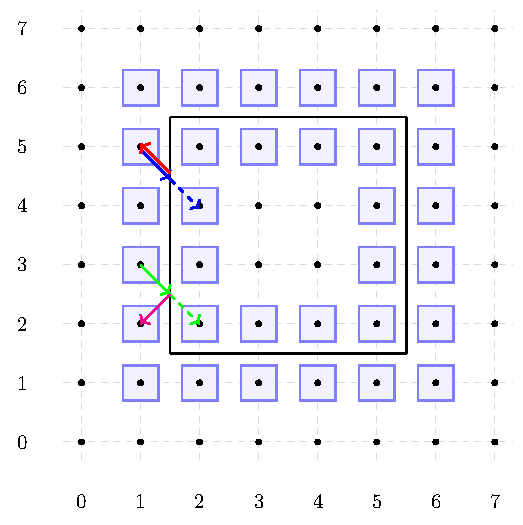
\includegraphics[]{imgs/cqlbm/bounceback_plaatje.pdf}
    \caption{Illustration of bounce back boundary conditions (top, in red and blue arrows) versus specular reflection boundary conditions (bottom, in green and magenta).}
    \label{fig:bounce_back_vs_specular_reflection}
\end{figure}

For implementing the bounce back boundary condition as a quantum primitive we require only one ancilla qubit $a_{o}$ to indicate whether a particle has virtually moved into an object. The ancilla $a_{o}$ is initialized in the $\ket{0}$ state and flipped to $\ket{1}$ when a particle has virtually travelled into one of the points inside the obstacle. We check whether a particle has virtually travelled into the object using the efficient object encoding method as described in Section \ref{sec:complete quantum specular reflection step}. 

As a next step we flip the state of the $v_\text{dir}^j$ qubits for all dimensions $j$ controlled on the state of the $a_o$ ancilla. By doing this we make sure that the velocity direction is reversed in all dimensions after contact with an obstacle as is required for bounce back boundary conditions. And subsequently the particles are moved by one position controlled on the $a_v^j$ , $v_\text{dir}^j$ and $a_o$ qubits to ensure that the particles move one step in the correct direction in the dimension(s) that they moved in when they moved into the obstacle and of course to ensure that this only happens after the particles moved into the obstacle. 

Finally the $a_o$ qubits need to be reset to $\ket{0}$ before we can start the next time step. As in Section \ref{sec:complete quantum specular reflection step} the blue and green encircled points outside of the object constitute the trivial case in Figure \ref{fig:example_right}. We reset the $a_o$ qubits controlled on if we are in one of the blue (green) encircled points, the direction of the $x$ ($y$) velocity and the ancilla qubit indicating whether we moved in the dimension in this time step $a_v^1$ ($a_v^2$). Specifically we reset the ancilla qubit $a_o$ if we are in a blue (green) encircled grid point outside the object and $a_v^1 = 1$ ($a_v^2 = 1$) and $v_\text{dir}^1$ ($v_\text{dir}^2$) points away from the object. Using this logic the $a_o$ qubits are reset to $\ket{0}$ for each wall separately.

Resetting the $a_o$ qubit is a bit more difficult around the edges as indicated with black and orange encircled points in Figure \ref{fig:example_right}. 

For the black encircled points outside the corner we need to reset the ancilla qubit $a_o$ if and only if both $v_\text{dir}^1$ and $v_\text{dir}^2$ point in the direction away from the object and $a_v^1 = a_v^2 =1$ holds.

As for the orange encircled `side-edge' grid point we first reset the $a_o$ ancilla in the same way as for the blue (green) encircled points described above. Now we only need to note that for the case described by the red arrow in Figure \ref{fig:example_right} we have wrongly flipped the $a_o$ ancilla qubit and so we need to verify whether we are in the `red arrow' case by checking if $v_\text{dir}^1$ and $v_\text{dir}^2$ pointed in the direction of the arrow and if $a_v^1 = a_v^2 =1$ holds. If the particle is in a state where  $a_v^1 = a_v^2 =1$ and $v_\text{dir}^1$ and $v_\text{dir}^2$ are such that the particle is in an red arrow case the $a_o$ ancilla get flipped again, back to the original state of $\ket{0}$. 

\begin{figure}[h]
    \centering
    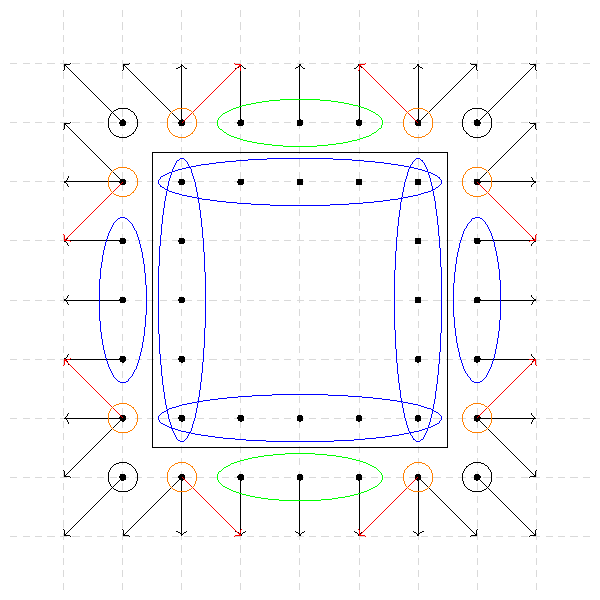
\includegraphics[]{imgs/cqlbm/corner_cases_bb.pdf}
    \caption{Illustration of all possible corner cases to be taken into account when particles collide with an obstacle (black box) and the physically correct behavior for a fail-safe implementation of boundary conditions.}
    \label{fig:example_right}
\end{figure}


\section{Quantum momentum exchange method}\label{sec:QMEM}
In this section we explain how the momentum exchange method can be expressed as an observable for the encoding described in Section \ref{sec:quantum register set-up}. In order to do this we will first change the density encoding of the quantum state into a rooted density encoding. Using this rooted density encoding we can subsequently define the observable that calculates the force using Equation \eqref{eq:F2} and finally we describe how this method can be implemented as an executable quantum circuit.

\paragraph*{Rooted density encoding}\label{subseq:rooted}
Since the momentum exchange method is linear in nature, whereas quantum observables are quadratic, it is advisable to change from encoding the density function $ f_i \left  (\mathbf{x},t \right ) $ in the quantum state $\ket{\psi}$ to an encoding of the square root of the density function $\sqrt{ f_i \left ( \mathbf{x}, t \right ) }$. Such a shift to a rooted density encoding can be done without altering any subsequent circuits in the methods \cite{Schalkers2022, Todorova2020}. 


\subsection{Momentum exchange method as an observable}\label{subseq:obs}
We now derive the observable that calculates the force exerted on the object using the momentum exchange method. As force is described using a vector, we need to calculate the values of the vector for all $d$ dimensions. Here we show how to calculate this vector using $2d$ different observables, where each observable calculates the value of the force vector in one spatial dimension, $d\in\{1,2,3\}$, and one velocity direction. This is done to make the resulting observable easier to portray and explain, since all the observables can be expressed as diagonal matrices they do commute and so they can all be measured in the same runs. 

Considering the encoding described above, Equation \eqref{eq:F2} can be evaluated from the quantum state $\ket{\psi}$ encoding $\sqrt{ f_i \left (\mathbf{x},t \right )}$, by the diagonal observable $O_{\text{OME}}$ to be specified below. The diagonal of the matrix expressing the observable $O_\text{OME}$ is built up using $B_{\text{OME}}$ matrices, which are placed at grid points in the fluid domain directly adjacent to the obstacle. All the other indices of the matrix matrix expressing $O_{\text{OME}}$ will remain zero. An example of this is the matrix
\begin{equation}\label{eq:Obs_1}
        O_{\text{OME}} = \begin{bmatrix}
            \dots & \dots & \dots & \dots  \\
            \dots &  B_{\text{OME}} & \dots & \dots \\
            \dots & \dots & \dots & \dots \\
            \dots & \dots & \dots & \dots \\
        \end{bmatrix},
\end{equation}
where the dots represent $4 \times 4$ matrices with only 0 indices and $B_{\text{OME}}$ is a $4 \times 4$ matrix that can be written as 
\begin{equation}\label{eq:bmatrix}
    B_{\text{OME}} = \begin{bmatrix}
        0 & 0 & 0 & 0\\
        0 & 0 & 0 & 0 \\
        0 & 0 & 2 & 0 \\
        0 & 0 & 0 & 0 
    \end{bmatrix}.
\end{equation}
The example given in Equation \eqref{eq:Obs_1} represents a 1-dimensional case with 4 grid points and three possible speeds (one in the positive and one in the negative $x$-direction as well as the zero speed) and the wall adjacent to the second grid point as represented in Figure \ref{fig:D1Q3ex_obs}. Since $B_{\text{OME}} = B_{\text{OME}}^{\dagger}$, both $B_{\text{OME}}$ and $O_{\text{OME}}$ are Hermitian and therefore $O_{\text{OME}}$ constitutes a quantum observable. It can easily be seen that any other distribution of $B_{\text{OME}}$ along the diagonal will also lead to a quantum observable. 

\begin{figure}[h]
    \centering
    
\includegraphics[]{imgs/cqlbm/four_gp_1_box.pdf}
\caption{Example of the D1Q3 case with four grid points and one obstacle located on the third grid point.}
\end{figure}\label{fig:D1Q3ex_obs}

For the D1Q3 case with four grid points described above we have the following quantum state encoding \begin{equation} \ket{\psi} = \frac{1}{\sqrt{\sum_{x,i} f_i \left (\mathbf{x},t \right )}} \sum_{x,i} \sqrt{ f_i \left (\mathbf{x} ,t \right )}\ket{g^1_2g^1_1v^1v^1_\text{dir}},
\end{equation} where $g^1_2g^1_1$ represent the binary value of the location of the $x$-axis, $\ket{v^1v^1_\text{dir}} = 01$ indicates streaming in the positive $x$-direction, $\ket{v^1v^1_\text{dir}}=11$ indicates streaming in the negative $x$-direction and $\ket{v^1v^1_\text{dir}}=01$ as well as $\ket{v^1v^1_\text{dir}}=00$ indicates that the particle is not streaming in the $x$-direction. Here and in the remainder of this Section we do not take into account the ancilla qubits as they play no role in the final density function and as such will not be part of the measurement process.

With the above convention, the quantum state can be written as the coefficient vector relative to the computational basis as follows: 
\begin{equation}\label{eq:psi}
    \ket{\psi} = \sum_{x,v} \alpha_{x,v} \ket{g^1_2g^1_1v^1v^1_\text{dir}} = \frac{1}{\sqrt{\sum_{x,i} f_i \left (\mathbf{x},t \right )}} \begin{bmatrix}
        0 \\
        \sqrt{f_0(0,t)} \\
        \sqrt{f_1(0,t)} \\
        \sqrt{f_2(0,t)} \\
        0 \\
        \sqrt{f_0(1,t)} \\
        \sqrt{f_1(1,t)} \\
        \sqrt{f_2(1,t)} \\
        0 \\
        \sqrt{f_0(2,t)} \\
        \sqrt{f_1(2,t)} \\
        \sqrt{f_2(2,t)} \\
        0 \\
        \sqrt{f_0(3,t)}  \\ 
        \sqrt{f_1(3,t)} \\
        \sqrt{f_2(3,t)}         
        % \sqrt{f(0,v_0)} \\
        % \sqrt{f(0,v_1)} \\
        % \sqrt{f(1,v_0)} \\
        % \sqrt{f(1,v_1)} \\
        % \sqrt{f(2,v_0)} \\
        % \sqrt{f(2,v_1)} \\
        % \sqrt{f(3,v_0)} \\
        % \sqrt{f(3,v_1)}      
    \end{bmatrix}.
\end{equation}
Using expression \eqref{eq:psi} and some basic linear algebra it follows that
\begin{equation}\label{eq:obs_value}
    \braket{\psi|O_{\text{OME}}|\psi} = \frac{2f_1 \left ( 1, t \right )}{\sum_{x,i}f_i \left (\mathbf{x},t \right )} .
\end{equation}
Since the value of $\sum_{x,i}f_i \left (\mathbf{x},t \right )$ is known when starting the algorithm we can simply multiply Equation \eqref{eq:obs_value} by $\sum_{x,i}f_i \left (\mathbf{x},t \right )$ to find the value of the force we wish to calculate as described in Equation \eqref{eq:F2}, which can subsequently be used to calculate the drag and lift coefficient \cite{Ladd1994}. 

\paragraph*{Extension to more dimensions}
This method can easily be extended to more dimensions by noticing that the $B_\text{OME}$ matrix is of size $2^{n_v} \times 2^{n_v}$ and should consist of only one non-zero element. This non-zero element will always be placed on the diagonal at the position of the basis state $\ket{v^i}$. 

\paragraph*{Complexity Analysis}\label{sec:CA}
The number of measurements required to determine the force with an $\epsilon$ precision using our proposed approaches depends on multiple factors. 
As long as the total number of grid points located inside and adjacent to the boundary of the obstacle is polynomial in the total number of grid points, the number of diagonal elements that are non-zero in the observable is polynomial in the size of the grid. This means that the number of non-zero elements in the observable is not exponentially small in the total size of the system. Therefore, in this case, we wish to measure a subspace that is only polynomially small in the total size of the system which is feasible without exponential overhead. 

\subsection{Practical implementation of the momentum exchange method on a quantum computer}\label{sec:prac_impl}
Realizing an observable on a real-world quantum computer amounts to implementing a quantum circuit that translates the observable to measurements in the computational Z-basis.
We will now present the quantum circuit that translates the observable described in Subsection \ref{subseq:obs} for determining the force in one dimension in one direction to measuring one qubit in the Z-basis, making the process clear and easily implementable on a quantum device. 

We will first describe how this operation can be applied by using an already implemented circuit for the bounce back boundary condition and we will subsequently show that this operation indeed transforms the described observable to one that consists of a Z measurement on one qubit. 

\subsubsection{Implementation using ancilla qubits for bounce back boundary conditions}
We have implemented a method to measure the expectation value of the described observable by measuring only one qubit. This is done using the implementation of the bounce back boundary conditions. In this implementation a qubit $a_{o}$ gets flipped to indicate that a particle is inside an object. To determine the expectation value of the observable we will use these ancilla qubits differently. We will from now on call this $a_{o}$ ancilla qubit that was used for the bounce back boundary conditions $a_{o,+}$ and we define a second ancilla qubit $a_{o,-}$. These ancilla qubits will be flipped if a force was exerted on the object in a positive or negative direction, respectively. In order to do this we apply a multi-controlled NOT operation controlled on the  qubits to determine whether we are in the object and the qubit indicating the direction of the particles in the dimension to the $a_{o,+}$ ($a_{o,-}$) qubits.  

By doing this we are extracting the relative density of particles that come into contact with an obstacle in the positive and negative direction for the considered dimension. Subsequently we measure the qubits $a_{o,+}$ and $a_{o,-}$ and subtract the expectation value of $a_{o,-}=1$ from $a_{o,+} = 1$. The resulting value expresses the relative pressure in the positive / negative direction. 

\subsubsection{Proof of method}
In this section we show that using the method described above, we indeed calculate the force exerted on an object in one dimension as expressed in Equation \eqref{eq:F2}.

We flip the $a_{o,+}$ ancilla qubit in the case that particles have impinged on the object and the particles have a positive velocity in the $x$-direction. %@Merel je hebt er hier x van gemaakt omdat het duidelijker lijkt dan steeds naar de desbetreffende dimensie te refereren. Pas dit later aan.
Therefore, after re-arranging some qubits, we can write 
\begin{equation}
\begin{split}
    & \bigl( \sqrt{f_{v_0} \left ( x_0,t \right )} \ket{ \left ( g_{n_g} \dots g_{1} \right )_0 \left (  v_{n_v} \dots v_1 \right )_0 } + \dots +   \\ & \sqrt{f_{v_1} \left ( x_1, t\right )} \ket{ \left (  g_{n_g} \dots g_{1} \right )_1 \left (  v_{n_v} \dots v_1 \right )_1} \bigr) \ket{0}_{a_{o,+}} +  \\ & \bigl( \sqrt{f_{v_2} \left ( x_2, t \right )}\ket{\left ( g_{n_g} \dots g_{1} \right )_2 \left ( v_{n_v} \dots v_1 \right)_2} + \dots +  \\  & \sqrt{f_{v_3} \left ( x_3 ,t\right )} \ket{ \left ( g_{n_g} \dots g_{1} \right )_3 \left ( v_{n_v} \dots v_1 \right )_3}  \bigr) \ket{1}_{a_{o,+}},
    \end{split}
\end{equation}
where for $v_i$ and $x_i$  the subscript is simply used to indicate that a specific value for the location and velocity is considered and similarly for the qubits $\left ( g_{n_g} \dots g_{1} \right )_i$ $\left (  v_{n_v} \dots v_1 \right )_i$ the subscript is used to indicate the velocity and grid point qubits are in a specific state. 
Here the states $ \ket{ \left ( g_{n_g} \dots g_{1} \right )_0 \left (  v_{n_v} \dots v_1 \right )_0 } + \dots +  \ket{\left (  g_{n_g} \dots g_{1} \right )_1 \left (  v_{n_v} \dots v_1 \right )_1}$ describe exactly the particles that do not impinge on the object in the positive $x$-direction in the current time step, as the $a_{o,+}$ qubit is in the $\ket{0}$ state. Similarly the states $\ket{\left ( g_{n_g} \dots g_{1} \right )_2 \left ( v_{n_v} \dots v_1 \right)_2} + \dots + \ket{\left ( g_{n_g} \dots g_{1} \right )_3 \left ( v_{n_v} \dots v_1 \right )_3}$ represent the relative densities of the particles that have impinged the object in the positive $x$-direction.
From this we can conclude that the total probability of finding $\ket{a_{o,+}} = \ket{1}$ upon measurement is equal to \begin{equation}
    f_{v_2} \left ( x_2, ,t\right ) + \dots + f_{v_3} \left ( x_3,t \right ),
\end{equation}
which is precisely equal to the relative density of particles hitting the object with a positive velocity and which is precisely what we wish to measure. 


% =============================================================================
\section{Data encoding}\label{sec:proof}
As in any computational field, data encoding is pivotal for reaching a good result. More than five decades of classical CFD research and application have established `good practices' for storing field data such as densities and velocities at, e.g., the grid points or cell centers as floating-point numbers following the IEEE-754 standard. Every now and then new hardware developments stimulate research into non-standard formats, like reduced or mixed-precision \cite{Freytag2022}, but, in general, data encoding is not considered to be an open problem.

Not so in QCFD and, in particular, quantum Boltzmann methods. In this section we will review the main data encodings currently used for QBM and show that in all of them either the streaming step or the collision step cannot be unitary. This result, though discouraging at first sight, should be interpreted as wake-up call that novel quantum encodings for CFD states are imperative for devising full-fledged QCFD applications in the future. We propose one such novel encoding in Section \ref{sec:novel_encoding} and discuss its potential and limitations.

The two mainstream encodings of the velocity vector are the amplitude based encoding and the computational basis state encoding. In what follows, we will consider both approaches separately and show how they both lead to a contradiction in the unitarity of either the collision or the streaming operation. 

\subsection{Amplitude based encoding}\label{ssec:amplitude_based_encoding}
The first type of encoding we consider is the so-called amplitude based encoding, used for several quantum Boltzmann methods \cite{Todorova2020, Budinski2020, Budinski2021, Schalkers2022}.
The amplitude based encoding of the velocity vector is such that at each location $\ket{x}$ there can be multiple particles with different velocities, for instance $\ket{v_0}$, $\ket{v_1}$, $\ket{v_2}$ and $\ket{v_3}$ for D2Q4. Here and below, $\ket{i}$ denotes the representation of $i$ as bit string. The state of the system at this point $x$ can then be encoded as\footnote{Note that we distinguish in our notation between the grid point $x$ and its representation $\ket{x}$ as part of the quantum register.}
\begin{equation}
\ket{x}\left (\alpha_0\ket{v_0} + \alpha_1\ket{v_1} + \alpha_2\ket{v_2} + \alpha_3\ket{v_3} \right ),
\end{equation}
where $\alpha_0$, $\alpha_1$, $\alpha_2$ and $\alpha_3$ are complex numbers that simply represent the relative weight or amount of particles traveling at the given velocity at grid point $x$. For simplicity we will assume that $|\alpha_0|^2+|\alpha_1|^2+|\alpha_2|^2+|\alpha_3|^2=1$, and so in this example there are only particles at grid point $x$ but the proof extends trivially to the general case with particles spread around the grid.

In order to show that this encoding of the velocity vector inevitably leads to non-unitary collision operators, let us assume a system in a specific state $\ket{\psi_1}$, with only particles traveling with velocities $\ket{v_0}$ and $\ket{v_1}$, meaning that $|\alpha_0|,|\alpha_1| > 0$ and $\alpha_2=\alpha_3=0$. Then we can write the state of the system as
\begin{equation}\label{eq:sys1}
\ket{\psi_1} = \ket{x}\left (\alpha_0\ket{v_0} + \alpha_1\ket{v_1} \right ).
\end{equation}
Now assume that an equivalent velocity combination exists consisting of particles traveling with velocities $\beta_2\ket{v_2} + \beta_3\ket{v_3}$, where we have $|\beta_2|,|\beta_3| > 0$. To realize this potential outcome of a collision as a quantum algorithm, we need to implement the transformation between both equivalent states as a unitary operation
$U_\text{col}$ which changes the states of the velocity encodings as follows
\begin{equation}
\begin{split}
     \ket{\psi_1^\prime} &= I \otimes U_\text{col} \ket{\psi_1} \\& = \ket{x}\otimes U_\text{col}\left (\alpha_0\ket{v_0} + \alpha_1\ket{v_1} \right ) \\ & =\ket{x} \left ( \gamma_0(\alpha_0\ket{v_0} + \alpha_1\ket{v_1}) + \gamma_1(\beta_2\ket{v_2} + \beta_3\ket{v_3})  \right ).
\end{split}
\end{equation}
Here, if $\gamma_0=1$ and $\gamma_1=0$ no collision is taking place (and we simply implement an identity operation) and if $\gamma_1=1$ we fully change from the original velocities to its alternative representative from the same equivalence class.\footnote{Here $\gamma_0$, $\gamma_1$ are chosen to reflect the fact that a collision operation should switch weight of a combination of velocities in an equivalent class to another combination of velocities in the same equivalence class. This equation could be written in a less restrictive way by splitting $\gamma_0$ and $\gamma_1$ up into separate amplitudes $\gamma_i$ for all the basis states $\ket{v_i}$, the same contradiction of unitarity as presented below however could be reached.} Note that to preserve unitarity $|\gamma_0|^2+|\gamma_1|^2=1$ must hold.

Let us now consider another system in state $\ket{\psi_2} = \ket{x}\ket{v_2}$. Applying the unitary operation $U_\text{col}$ should not effect the state at all as a single speed is only in an equivalence class with itself, and so the required behavior for $U_\text{col}$ is
\begin{equation}\label{eq:sys2_end}
\begin{split}
     \ket{\psi_2^\prime} &=I \otimes U_\text{col}\ket{\psi_2} \\ & =  \ket{x}U_\text{col}\ket{v_2} \\ & = e^{i\theta}\ket{x}\ket{v_2},
\end{split}
\end{equation}
with $\theta\in (0,2\pi]$. That is, the collision operator must preserve the single-velocity state except for changes in the phase factor $e^{i\theta}$ that can be neglected.

Now that we have identified the required behavior for $U_\text{col}$ to implement a collision operation, we can prove that any $U_\text{col}$ that meets both requirements simultaneously cannot be unitary. Here, we resort to the characterization $U_\text{col}^\dagger U_\text{col}=I$ of unitary operators, with superscript $\dagger$ denoting the adjoint operator.

\begin{proof}
To reach a contradiction, assume that $U_\text{col}$ is a unitary operator. Then it must preserve the inner product for all possible states $\ket{\phi_1}$ and $\ket{\phi_2}$
\begin{equation}
    \braket{\phi_1 | \phi_2} = \bra{\phi_1} U_\text{col}^\dagger U_\text{col} \ket{\phi_2}.
\end{equation}

However, for a collision operation $U_\text{col}$ that behaves as expected on the system states described in Equations \eqref{eq:sys1} to \eqref{eq:sys2_end}, it follows that
\begin{equation}
\begin{split}
0 &=\braket{\psi_1|\psi_2} \\ & = \bra{\psi_1} \left ( I \otimes U_\text{col} \right )^\dagger \left ( I \otimes U_\text{col} \right ) \ket{\psi_2} \\ & = e^{i\theta}\left ( \gamma_0(\alpha_0\bra{v_0} + \alpha_1\bra{v_1}) + \gamma_1(\beta_2\bra{v_2} + \beta_3\bra{v_3})  \right )  \bra{x} \ket{x}  \ket{v_2}  \\ & = e^{i\theta}\gamma_1\beta_2.
\end{split}
\end{equation}
The first equality follows from the fact that $\ket{\psi_1}$ and $\ket{\psi_2}$ are orthogonal by construction. The second one holds under the assumption of $U_\text{col}$ being unitary, which is disproved by the fact that the entire equality chain only holds for the trivial case $\gamma_1=0$ (as $|\beta_2|>0$ by definition of the state $\ket{\psi_1}$), that is, when $U_\text{col}$ does not implement the collision operation.
From this we can conclude that an amplitude based encoding of the velocity does not allow for a unitary implementation of the collision operation. 
\end{proof}
Notice that this proof works for any amplitude based encoding of $v$ where the different possible velocities at a position are all represented by their own basis state as there will always be a case with only a single incoming velocity, for which an identity operation up to a phase shift should take place, while at the same time there will be combinations of velocities for which we want some weight of the system to change from one combination of velocities to another combination of velocities in the same equivalence class. These two antagonizing requirements will always lead to the same contradiction of unitarity proven above and we further expand on this intuition in Section \ref{ssec:intuition}.


\subsection{Computational basis state encoding}\label{ssec:comp_basis_encoding}
The second type of encoding of a quantum state considered is the computational basis encoding, used in several quantum lattice Boltzmann papers such as \cite{Yepez1998, Yepez2001, YepezBoghosian2001, Yepez2002, Pravia2003, Moawad2022, Steijl2023}. Using this encoding the contradiction of unitarity in the collision operation can be avoided by encoding the velocity of the qubits at a position $\ket{x}$ in space by identifying each direction particles could be streamed from with its own qubit, which will be set to one if and only if there is a particle streaming from that direction.

As an example consider the D2Q4 lattice depicted in Figure \ref{fig:D2Q4_ex}. In this case the velocity can be encoded using four qubits $q_0$, $q_1$, $q_2$ and $q_3$ where the state
\begin{equation}
    \ket{x}\ket{v} = \ket{x}\ket{q_0q_1q_2q_3} = \ket{x}\ket{0110}
\end{equation}
is such that from the center point $(1,1)$, there is a particle streaming to $(1,2)$ and a particle streaming to $(0,1)$ but not to $(2,1)$ or $(1,0)$. 

\begin{figure}[h]
\centering
    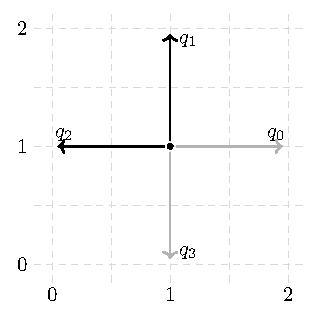
\includegraphics[]{imgs/space_time/D2Q4_ex.pdf}
    \caption{Illustration of the computational basis state encoding for the D2Q4 lattice. For each grid point $x$ we set the respective qubit $q_j$ to one if and only if there is a particle streaming in that direction, i.e. $\ket{v} = \ket{q_0q_1q_2q_3} = \ket{0110}$.}
    \label{fig:D2Q4_ex}
\end{figure}

Using this encoding the collision step can be defined quite naturally as unitary operation. However, we run into trouble when attempting to define a unitary streaming step $U_\text{str}$ as we demonstrate in what follows. 

To simplify notation let us restrict ourselves to the D1Q2 lattice and consider the two settings at time $t$ from Figures \ref{fig:D1Q2ex_1} and \ref{fig:D1Q2ex_2}, which can be encoded as
\begin{align}
    \ket{\psi_1} &= \sum_{x=0}^3 \ket{x}\ket{v}\\ &= \frac{1}{2}\left ( \ket{00}\ket{00} + \ket{01}\ket{11} + 
\ket{10}\ket{10} + \ket{11}\ket{10}\right ),
\label{eq:psi1_str}
\end{align}
and 
\begin{equation}
    \ket{\psi_2} = \frac{1}{2} \left ( \ket{00}\ket{01} + \ket{01}\ket{01} + 
\ket{10}\ket{00} + \ket{11}\ket{11} \right ),
\label{eq:psi2_str}
\end{equation}
respectively. It then follows directly that 
\begin{equation}
    \braket{\psi_1|\psi_2} = 0.
    \label{eq:orthogonal}
\end{equation}

Upon streaming, the systems from Figures \ref{fig:D1Q2ex_1} and \ref{fig:D1Q2ex_2} change from their state at time $t$ (top lattice) to that at time $t+1$ (bottom lattice), i.e.
\begin{equation}
    \ket{\psi_1^\prime} = \frac{1}{2} \left ( \ket{00}\ket{11} + \ket{01}\ket{00} + 
\ket{10}\ket{10} + \ket{11}\ket{10} \right ),
\label{eq:psiprime1_str}
\end{equation}
and 
\begin{equation}
    \ket{\psi_2^\prime} = \frac{1}{2} \left ( \ket{00}\ket{11} + \ket{01}\ket{00} + 
\ket{10}\ket{01} + \ket{11}\ket{01} \right ) ,
\label{eq:psiprime2_str}
\end{equation}
respectively. As in the previous section, we will show by contradiction that any operation $U_\text{str}$ for which $U_\text{str}\ket{\psi_1} = \ket{\psi_1^\prime}$ and $U_\text{str}\ket{\psi_2} = \ket{\psi_2^\prime}$ cannot be unitary. 

\begin{proof}
    Let us assume that $U_\text{str}$ is unitary, i.e. it preserves the inner product
    \begin{equation}
        \braket{\phi_1 | \phi_2} = \bra{\phi_1} U^\dagger_\text{str} U_\text{str} \ket{\phi_2},
    \end{equation}
for all states $\ket{\phi_1}, \ket{\phi_2}$. Substituting the states \eqref{eq:psi1_str} and \eqref{eq:psi2_str} on the left side, and \eqref{eq:psiprime1_str} and \eqref{eq:psiprime2_str} into the right inner product we arrive at the contradiction 
\begin{equation}
    0=\braket{\psi_1 | \psi_2} = \bra{\psi_1}U_\text{str}^\dagger U_\text{str} \ket{\psi_2} =
    \braket{\psi_1^\prime | \psi_2^\prime} = \frac{1}{2}.
\end{equation}
The first equality follows from the orthogonality property \eqref{eq:orthogonal}, and the second one from the assumption that $U_\text{str}$ is a unitary operator, which we just disproved.
\end{proof}

\begin{figure}
    \centering
     \begin{minipage}{.47\textwidth}
         \centering
    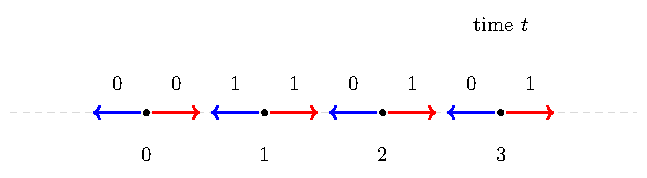
\includegraphics[]{imgs/space_time/D1Q2ex_1_1_t.pdf}
         \label{fig:D1Q2ex_1_1}
    \vspace{.5cm}
    \end{minipage}
    \begin{minipage}{.47\textwidth}
        \centering
    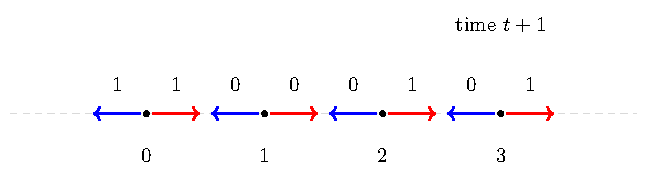
\includegraphics[]{imgs/space_time/D1Q2ex_1_2_t.pdf}
         \label{fig:D1Q2ex_1_2}
     \end{minipage}
    
    \caption{D1Q2 example setting 1. The binary encoding above the arrows indicate whether or not a particle is flowing there in that time step. 1 indicates that there is a particle streaming there and 0 indicates that there is no particle. In the example setting we consider periodic boundary conditions. The top figure shows the state of the system at time $t$. The figure below shows the state of the system at time $t+1$.}
    \label{fig:D1Q2ex_1}
\end{figure}

\begin{figure}
         \centering
     \begin{minipage}{.47\textwidth}
         \centering
        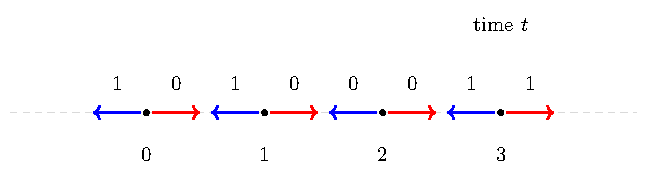
\includegraphics[]{imgs/space_time/D1Q2ex_2_1_t.pdf}
         \label{fig:y equals x}
    \vspace{.5cm}
     \end{minipage}
     \begin{minipage}{.47\textwidth}
         \centering
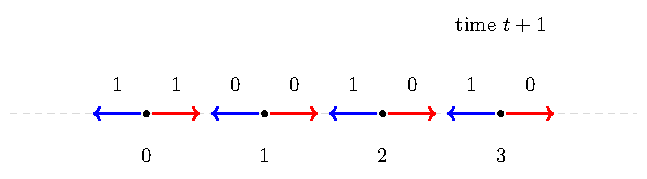
\includegraphics[]{imgs/space_time/D1Q2ex_2_2_t.pdf}
         \label{fig:three sin x}
     \end{minipage}
    \caption{D1Q2 example setting 2, the binary encoding above the arrows indicate whether or not a particle is flowing there in that time step. 1 indicates that there is a particle streaming there and 0 indicates that there is no particle. In the example setting we consider periodic boundary conditions. The top figure shows the state of the system at time $t$. The figure below shows the state of the system at time $t+1$.}
    \label{fig:D1Q2ex_2}
\end{figure}

As in Section \ref{ssec:amplitude_based_encoding} this proof extends to any computational basis encoding where each possible combination of velocities at a specific lattice point is encoded using its own basis state, as one can always construct two situations with no overlap at time $t$ that will have non-zero overlap after streaming at time $t+1$. This proof also extends trivially to any other D$d$Q$q$ setting as the streaming possibilities of D1Q2 are essentially a subset of any other system and thus the same example can be used by setting the other streaming directions to 0.


\subsection{Intuition and extension of non-unitarity proofs}\label{ssec:intuition}
In this section we expand on our non-unitarity proofs by providing physical intuition behind the proofs presented above. It is intended to give insight into what types of encodings our non-unitarity proof extends to, and what physical features of the system necessarily lead to the non-unitarity for these encodings. 

Consider the proof from Section \ref{ssec:amplitude_based_encoding} that shows that the amplitude based encoding, where each velocity direction is identified through its own basis state leaving the total velocity at a position $x$ to be a superposition of such basis states, prevents the collision operator $U_\text{col}$ from being unitary. Since it encodes each streaming direction as a different basis state, the quantum encodings of the velocity directions are all orthogonal to one another. This is also necessary, since if the basis states of the possible streaming directions are not orthogonal, we cannot fully distinguish between them. However, this orthogonality of the different velocity directions leads directly to the non-unitarity of $U_\text{col}$. Since a collision operator that will rotate a given linear combination of basis states into a linear combination of other basis states in such a way that the represented streaming patterns belong to the same equivalence class, it will also rotate `pure' velocities represented by a single basis state into another basis state leading to a nonphysical and undesired change of velocities. 

Following this line of argumentation it can be seen that the non-unitarity of $U_\text{col}$ is not so much a result of a specific choice of encoding but an inherent non-unitarity of the collision step itself that directly leads to the idea of computational basis state encoding, where each velocity pattern (i.e. the combination of velocities) at a grid point is encoded as its own basis state, and not as a unitary combination of all the basis states representing a non-zero contribution.

When encoding the velocity pattern at each grid point as a basis state, naturally, the non-unitarity of collision falls away and we can find a straightforward unitary operator to implement the collision step.
However, such an encoding will always lead to non-unitarity of streaming due to the non-local nature of a streaming operation. Consider an arbitrary point in space $x$ and imagine two different scenarios with two different combinations of speeds $\ket{v_1}$ and $\ket{v_2}$ at this point. Then the inner product between $\ket{x}\ket{v_1}$ and $\ket{x}\ket{v_2}$ must be 0, as these are different basis states. However, the velocity states of the systems at position $x$ in the next time step do not depend on the current velocity states in the lattice point. In fact, they only depend on the velocity states of the neighboring lattice points. Since the inner product of the states at the point $x$ at the next time step does not depend on the current states at the point $x$, in the next time step the velocity at the point $x$ of the two systems could be identical, and hence, the inner product could be one. There is no way of ensuring that this can only happen when the inner product at some other point $x^\prime$ of the systems was non-zero before as each grid point has velocity vectors in multiple directions determining its associated velocity basis state. 

This shows that any quantum encoding that successfully implements both streaming and collision as a unitary operation must belong to one of the following three types. The first type is an amplitude based type encoding, where the different velocities are not orthogonal and thus not entirely distinguishable. The second type is a computational basis state encoding where the non-locality of streaming is somehow avoided. The last type is a completely novel encoding method that avoids both non-unitarity problems entirely.
In the next section we will present precisely one such idea.


\section{Space-time data encoding}\label{sec:novel_encoding}
In this section we propose a novel space-time data encoding that enables unitary collision \emph{and} streaming at the same time. To the best of our knowledge, this is the first-of-its-kind start-to-end quantum Boltzmann algorithm that does not require measurement and quantum-state re-initialization after each time step.

In what follows, we adopt an extended computational basis state encoding, where at each location $x$ we take into account the velocities at all grid points in the vicinity of $x$. Here, `in the vicinity of $x$' means that a particle can theoretically reach the grid point $x$ within the number of time steps still to be performed before measurement. Mathematically speaking being `in the vicinity of $x$' means being, respectively, in the so-called extended von Neumann, Moore or hexagonal neighborhood of the point $x$, depending on the lattice structure.\footnote{The von Neumann neighborhood of extent $r$ defines the diamond-shaped set of points at a Manhattan distance of up to $r$ from the point $x$. It applies to, e.g., D2Q4, D2Q5, D3Q6, and D3Q7. The Moore distance extends the former one by diagonal directions and applies to, e.g., D2Q8, D2Q9, D3Q26, and D3Q27. As its name suggests, the hexagonal neighborhood applies to D2Q6 and its extension to its three-dimensional counterpart.} 

This leads to a trade-off between the number of time steps that can be performed between measurements and the number of qubits required to encode the velocity at each grid point $x$. The more time steps one wishes to take between measurement-and-re-initialization cycles, the more qubits are required for our space-time encoding. Obviously the maximum number of qubits required to implement the velocity without any in-between measurements must be such that the entire grid is spanned. For a D$d$Q$q$ lattice this will be $qN_g$, where $N_g$ is the total number of grid points. When encoding the proposed method on a classical computer $qN_g$ bits would also be required, so when encoding the full domain there is no quantum benefit in terms of (qu)bit numbers. The quantum improvement comes from exploiting quantum parallelism, which is done as long as we do not encode the whole space.

In what follows, let $N_t$ denote the number of streaming steps to be performed between (re-)initialization and measurement. We extend the computational basis state encoding of velocity directions from Section \ref{ssec:comp_basis_encoding} to take into account all the speed states from grid points in the neighborhood of $x$ that can (at least theoretically) reach $x$ within $N_t$ streaming steps. This takes away the non-locality of the streaming operator, which led to the non-unitarity of $U_\text{str}$ for the `regular' computational basis state encoding at the cost of increasing the number of qubits required to encode all required velocity data.

We will give a detailed description of this encoding for the D2Q4 lattice, but want to note that it can be extended naturally to any other choice of D$d$Q$q$. Consider the D2Q4 lattice given in Figure \ref{fig:D2Q4} with qubit $q_j$ set to one if and only if there is a particle traveling with velocity direction $j$ from grid point $x$ into a neighboring grid point in the current time step. We now extend this encoding to include \emph{all} possible velocities at positions `in the vicinity of $x$' for the total of $N_t$ time steps in order to obtain a unitarily streamable encoding. This is illustrated in Figure \ref{fig:D2Q4_quantum} for a single time step, i.e. $N_t=1$ yielding the encoding
\begin{equation}
    \ket{x}\ket{q_{19}q_{18} \dots q_0}.
\end{equation}
For D2Q4, the number of qubits encoding the possible velocity states per grid location $x$ grows with the number of time steps (still) to be taken as
\begin{equation}\label{eq:von_Neumann}
    n_v = 4 + \sum_{i=1}^{N_t}16i = 8N_t^2 + 8N_t + 4,
\end{equation}
where the maximum number of qubits required to encode all velocity directions over the entire grid equals $4N_g$ as stated before.\footnote{Note that the growth rate of qubit numbers per time step depends on the choice of D$d$Q$q$. The number of qubits required is equal to the number of points in the extended Von Neumann, Moore or hexagonal neighborhood, depending on which choice of $d$ and $q$ considered.}
Similarly it can be shown that for $d$ dimensions the growth rate is of the order $\mathcal{O}\left (N_t^d \right)$.

We can now encode the collision step by first identifying the equivalence class for the D2Q4 lattice. We note that at each grid point $x$ as represented in Figure \ref{fig:D2Q4} the states $\ket{q_0q_1q_2q_3} = \ket{1010}$ and $\ket{q_0q_1q_2q_3} = \ket{0101}$ belong to the same equivalence class (cf. Figure \ref{fig:equivalence_class}), as they have the same total mass and momentum.\footnote{The other equivalence classes are $\ket{q_0q_1q_2q_3} = \ket{1000}$ and $\ket{q_0q_1q_2q_3} = \ket{1100}$ and all cyclic shifts of these patterns, and $\ket{q_0q_1q_2q_3} = \ket{1111}$. However, they all have just a single representative so that we define the collision operator based on the ambiguous case.} We implement the collision step by defining a unitary operator $U_\text{col}$ which performs the following mappings 
\begin{align}
    U_\text{col}\ket{1010} &= \phantom{-}\alpha\ket{1010} + \beta\ket{0101},\\
    U_\text{col}\ket{0101} &= -\beta\ket{1010} + \alpha\ket{0101},
\end{align} 
with $\alpha, \beta \in \mathbb{C}$ and $|\alpha|^2+|\beta|^2=1$,
while acting as the identity operation on any other basis state. It can easily be verified that this operation is unitary. With the so-defined $U_\text{col}\in \mathbb{C}^{2^4 \otimes 2^4}$, we can write the total collision operation for an encoding of the velocities states $v$ consisting of $n_v=4k$ qubits as $k$-fold Kronecker products of $U_\text{col}$ operations, i.e.  $U_\text{col}^\text{tot}=U_\text{col} \otimes \dots \otimes U_\text{col}$. Since each $U_\text{col}$ requires a few CNOT and a single triple controlled rotation gate the total collision operator can be efficiently implemented even on near-term devices.\footnote{We can implement the described collision operator by first applying three CNOT operations to the system turning the states into $\ket{1010} \mapsto \ket{1110}$ and $\ket{0101} \mapsto \ket{1111}$. Subsequently a triple controlled rotation operation of choice is applied to the right-most qubit (controlled on the three left-most qubits). Finally the initial three CNOT operations are applied in reverse order to reset all velocity states correctly.}

In practice the total collision operator $U_\text{col}^\text{tot}$ differs per time step, since its local counterpart $U_\text{col}$ only needs to be applied to velocity states `in the vicinity of $x$'. 
In the first out of the $N_t$ time steps it is important for all qubits representing velocity states `in the vicinity of $x$' to be updated correctly. In the very last time step, however, it is only important for the qubits $q_0$, $q_1$, $q_2$ and $q_3$ to end up in the correct state. The more time steps $t$ have been taken, the less time steps $N_t-t$ are still to be taken and so the 4-qubit local collision operator $U_\text{col}$ only needs to be applied to the remaining qubits relevant for encoding the `directly connected' velocity states as given in Equation \eqref{eq:von_Neumann}. 

With this logic we can define a collision operator per time step $t$ as
\begin{equation}
U_{\text{col},t}^\text{tot}=\underbrace{U_\text{col} \otimes \dots \otimes U_\text{col}}_{\text{$c$  collision operations}} \otimes \underbrace{I \otimes \dots \otimes I}_{\text{identity operations}},
\end{equation}
where $c = 2(N_t-t)^2 + 2(N_t-t) +1$ and the identity operations are added to avoid dimensionality issues. In practice no operation will be applied on the qubits encoding velocity states not `in the vicinity of $x$' within $N_t-t$ time steps. 

Our space-time encoding enables different manners of implementing the streaming step. It can easily be seen that the way the streaming method should be implemented differs per time step $t$ depending on which positions will be `in the vicinity of $x$' in the next time step as well. At the first time step it is important for (almost) all qubits to be streamed to a very specific position, whereas in the last time step it is only important for the qubits $q_0$, $q_1$, $q_2$ and $q_3$ to end up in the correct state. For the example shown below we are only considering a total of one step to be taken (i.e. $N_t=1$) and so we only need to consider the speeds that will stream to location $x$ in one time step. In this case that means that streaming consists of performing a swap operation between the following qubit pairs $q_0$ and $q_{12}$, $q_1$ and $q_{17}$, $q_2$ and $q_6$ as well as $q_3$ and $q_{11}$.  

Also in general (i.e. $N_t>1$), the streaming step can be implemented by a combination of swap gates. Following the same in-the-vicinity-of-$x$ argument as was used for the collision step, a total of 
\begin{equation}
n_\text{swap}(t) = 4+\sum_{i=1}^{N_t-t }16i = 8 \left ( N_t - t \right )^2 + 8\left ( N_t - t \right ) +4
\end{equation}
swap gates are required to update as many velocity-encoding qubits in time step $t$, whereby these swap operations can be performed largely in parallel.\footnote{In each time step the swap operations in the 4 (or generally speaking $q$) different directions can be performed in parallel. Furthermore the swap operations for the velocities in the same direction but not in the same `line of streaming' can all be performed in parallel. Therefore we only need to take into account the velocities in the same line of streaming and the depth of the circuit is determined by the longest `line of streaming', which is equal to $N_t-t$. In each layer of the swap operations at least half of the $N_t-t$ velocities can be swapped to the correct position. Therefore a total of $\log_2 \left (N_t-t \right )$ swap operations needs to be performed in the $t$-th time step.}
The depth of the streaming circuit at time $t$ will amount to 
\begin{equation}
    d_\text{str}(t) = \log_2 \left ( N_t-t \right )
\end{equation}
swap operations at time $t$. 


\begin{figure}[h]
\centering
    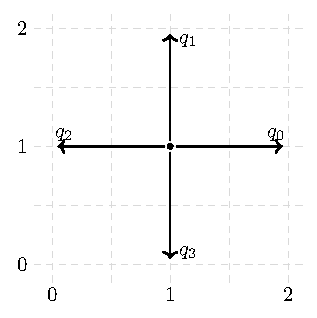
\includegraphics[]{imgs/space_time/D2Q4.pdf}
    \caption{Illustration of the computational basis state encoding for D2Q4.}
    \label{fig:D2Q4}
\end{figure}

\begin{figure}[h]
\centering
    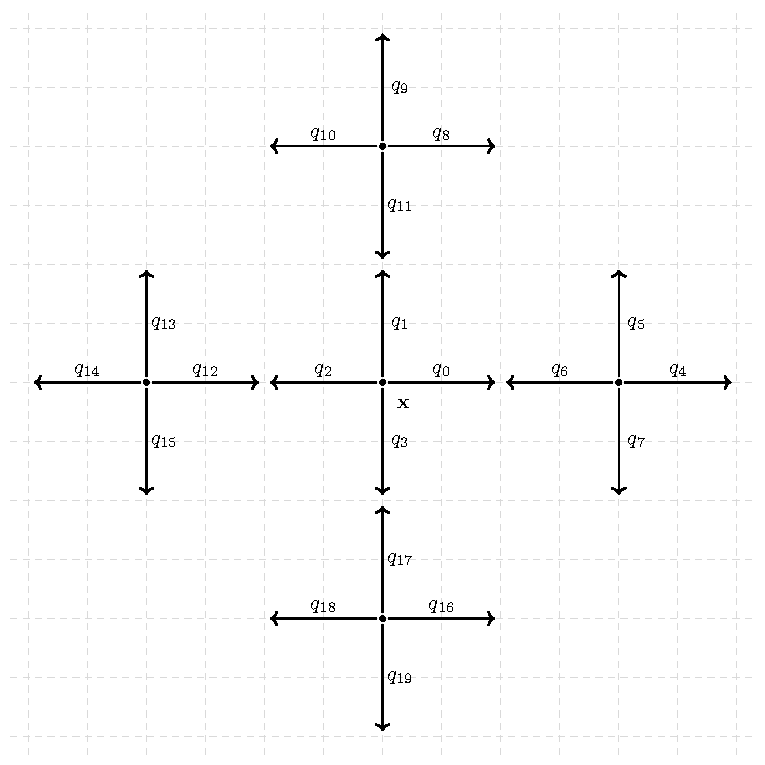
\includegraphics[]{imgs/space_time/D2Q4_quantum.pdf}
    \caption{Illustration of the space-time encoding for D2Q4 for a single time step.}
    \label{fig:D2Q4_quantum}
\end{figure}


% =============================================================================

\section{Comparison of our quantum Boltzmann methods to others}
In this section we will give a brief overview of how our quantum Boltzmann methods compare to the other main competitive methods out there. This section is meant to give insight into why certain design choices were made and how it improves the algorithm. In the appendix we furthermore provide a detailed complexity analysis of our CQBM compared to other implementations. 

\subsection{Collisionless Quantum Boltzmann methods - comparison}
Our approach furthermore improves over the original QBM \cite{Todorova2020} by Todorova and Steijl in several key manners. First of all our quantum specular reflection step, even though seemingly more complicated, performs the correct reflection behavior in all corner cases. This is not the case for the original QBM, which shows incorrect reflection behavior for particles hitting the corners of an obstacle on a non-axis-aligned trajectory. On top of that, our specular reflection approach also ensures that the particles are set back into the flow domain before the start of a new timestep if they virtually traveled into an object. This also avoids incorrect behavior present in the original QBM formulation.
Furthermore our approach for identifying the internal grid points of obstacles at which particles need to be reflected is more efficient than the method used by Todorova and Steijl. This leads to an additional polynomial speed-up.

We finally show that our quantum implementation of the streaming step outperforms the methods of \cite{Todorova2020, Budinski2020, Budinski2021} in terms of the the amount of CNOT gates required to implement them. We intentionally choose for the latter as performance measure as they are either available as native gates or can be efficiently emulated. Hence, complexity estimates in terms of CNOT gates give a more realistic picture of the costs on a real quantum computer, whereas complexity estimates in terms of multi-controlled gates conceal the costs for decomposing multi-controlled gates into native ones.

Last but not least our method outperforms the current state-of-the-art approaches in the encoding of the particles' velocity. We propose a novel encoding of the velocity vector, due to which velocities can be flipped with a single NOT operation performed on a single qubit, whereas before $n$ NOT operations were required to flip the direction of the velocity encoded using $n$ qubits \cite{Todorova2020}.

\subsection{Full quantum Boltzmann method - space time encoding compared to other methods}
There are other methods that have implemented both a streaming and a collision step for the Boltzmann equation. In this section we will compare our method to what we will refer to as 'stop-and-go' methods and the Carleman linearization method, which both allow for solving the full Boltzmann equation on a quantum computer. Specifically for the 'stop-and-go' method we will consider the method of Budinski described in \cite{Budinski2021} and for the Carleman linearization approach we will consider the paper \cite{Sanavio2023}. \\

We will first consider the method \cite{Budinski2021}, which requires measurement and reinitialization at the end of each time step. Both the measurement and reinitialization procedure are exponentially expensive for in the total number of qubits \cite{Shende2004}. This implies that any potential quantum advantage is lost when performing multiple timesteps. Next to that the initalization procedure itself might already be exponentially expensive in the first timestep, as the function that is encoded is in no way trivial to encode. Therefore even when performing one time-step it is impossible to make any promises of a non exponentially expensive initialization. \\
Furthermore the method of Budinski has no pre-determined quantum circuit for the implementation of the matrix that represents the collision operation. This means that for each timestep a block diagonal matrix $A$ consisting of $32 M \otimes M$ blocks has to be decomposed as a quantum circuit. Both the decomposition calculation and the final decomposed circuit might be exponentially expensive in the number of qubits that the block is applied to, which is another point where any potential quantum advantage might get lost even when performing only one timestep. 


The Carleman linearization function presented in \cite{Sanavio2023} also allows for solving the full Boltzmann equation on a quantum computer. Here first the so-called Carleman linearization is used to linearize the Boltzmann equation. The amount of Carleman variables required is of order $\mathcal{O} \left ( N^k Q^k \right )$, where $k$ is the truncation order \cite{Sanavio2023}. The challenge in this technique comes from then applying the linear operator that evolves the system per time step to the quantum state. This operator then consists of a $\mathcal{O} \left ( N^k Q^k \right )$ size matrix with a non-trivial decomposition, meaning a qiskit decomposition is required. Both the algorithm to decompose the unitary and the resulting circuit are potentially exponentially expensive. In the paper itself they also describe that performing this method for multiple time steps is currently too expensive due to the formidable depth of the resulting circuits.

The space-time encoding has two main benefits compared to the other methods. First of all, all the algorithmic procedures are naturally expressed in quantum gates. There is no need to decompose very large matrices into quantum gates, which as expressed before is exponentially expensive in both computation and potential outcome. The complexity of our streaming steps are $\mathcal{O} \left ( \left ( N_t - t \right )^2  \right )$ with a depth of only $\log_2 \left (N_t -t \right)$ where $N_t$ is capped by $N_g$ (where $N_g$ expresses the maximum number of grid points in a dimension). Furthermore the complexity of the collision step for the D2Q4 case is $\mathcal{O} \left ( \left ( N_t - t \right )^2  \right )$ with a depth of $9$.


% =============================================================================
% =============================================================================
\section{Conclusions}
In these lecture notes, we have discussed the main ideas behind the quantum Boltzmann method and quantum fluid dynamics as a whole. We have given an overview of the main methods of quantum computational fluid dynamics which are currently being developed. After which we have given an in-depth explanation of the Boltzmann equation and the subsequent computational methods. We have given a detailed explanation of the functioning of our collisionless quantum Boltzmann method and how it improves on other currently existing methods. For this method we have described an efficient measurement method that can be used to calculate the force exerted on an object. 

In the second half of these notes we have focused on the space-time encoding. We introduced this encoding by first deriving why none of the previously used encoding methods are suited to implement both collision and streaming as a unitary. We then used the logic behind these proofs to create an encoding that can be used to apply a streaming and collision operation to. This encoding, the so-called space-time encoding, currently outperforms the other known methods as explained in the final section. 


% =============================================================================
\section*{Acknowledgments}
We first and foremost want to thank C\u{a}lin Georgescu for proofreading and suggesting valuable changes to these lecture notes. Furthermore we gratefully acknowledge \textbf{Fujitsu Limited} and the \textbf{Netherlands Enterprise Agency} under project number PPS23-3-03596728 for financial support.

\bibliographystyle{nato-sto}
\bibliography{sections-2024/bib} % when using a BibTeX database -- and you should!

\appendix

\subsection{Complexity analysis\label{sec:comparison to state of the art}}
In this section we give a detailed complexity analysis of our collisionless quantum Boltzmann method (CQBM) algorithm. 
Since the most competitive quantum hardware can only implement single- and two-qubit gates natively \cite{Rigetti} \cite{IBM}, we decompose the multi-qubit operations into two-qubit gates to find a realistic quantum complexity for our method. Specifically we choose to give the complexity in terms of the CNOT gates, since these are native to IBM QPU. Though other vendors' QPUs have different native gate sets, e.g., Rigetti \cite{Rigetti}, the restriction to only one- and two-qubit gates holds for nearly all technologies of today. 

We subsequently compare our found complexity to the complexity for the current best known quantum algorithm for the collisionless Boltzmann equation \cite{Todorova2020}. In doing so we show that our method not only outperforms the current  by implementing the quantum reflection step in a fail-safe manner, but we also reach a better complexity.

\subsection{Complexity of multi-controlled NOT operations\label{ssec:multinot compl}}
In order to provide a cost analysis for our algorithm, we first need to determine the cost associated to implementing a multi-controlled NOT gate in terms of natively implementable 2-qubit gates. Specifically we will give the complexity of implementing multi-controlled NOT operations when decomposed in CNOT gates. While CNOT is one of the native gates for IBM QPUs \cite{IBM} it needs to be emulated by other two-qubit gates on other quantum hardware such as the QPUs from Rigetti \cite{Rigetti}. However, in these cases the CNOT gate can be decomposed using a fixed number of the natively implemented two-qubit gates, so this does not effect the overall complexity. 
Multiple ways of decomposing multi-controlled NOT gates into CNOT gates are known in literature. We distinguish several cases, one without ancilla qubits, one with a linear amount of ancilla qubits and multiple with a constant amount of ancilla qubits. \\

The method to decompose multi-controlled NOT gates into two-qubit operations without any ancilla qubits was given by Barenco et al. in \cite{Barenco1995}. The reported decomposition requires $48(p+1)^2 + \Theta(p)$ `basic operations'\footnote{Here the term basic operations implies either a CNOT or single qubit gate.}. From this we can deduce that approximately $c p^2$ with $22<c<48$ CNOT gates will be required for this method with complexity of $\mathcal{O}\left (p^2\right )$ CNOT gates. \\

With a linear amount of ancilla qubits we can use a more efficient decomposition in terms of CNOT gates required as described by Nielsen and Chuang in \cite{mikeandike}. For a multi-controlled operation with $p$ control qubits $p-1$ ancillae and $2(p-1)$ Toffoli gates\footnote{A Toffoli gate is a CCNOT gate, i.e., a controlled NOT gate with two control qubits.} are required. Each Toffoli gate in turn will be decomposed using 6 CNOT gates (and some other operations) \cite{mikeandike}. Therefore a total of $12(p-1)$ CNOT gates is required in combination with $p-1$ ancilla qubits to decompose a C$^p$NOT operation into native one- and two-qubit gates. \\

We can, however, also choose to use a constant amount of ancillae. 
The paper by Barenco et al. \cite{Barenco1995} provides a method to decompose C$^p$NOT operations for $p\geq 5$ using a single ancilla, $8(p-3)$ Toffoli gates and $ 48 (p+2)$ `basic operations' leading to $c p$ CNOT gates required to implement this method with $70 \leq c \leq 96$.

Another method we could use to implement a multi-control NOT gate using a single ancilla is by making use of the comparison operation. One can then find whether or not the $p$ control qubits are in the state $\ket{q_1 \dots q_k} = \ket{1 \dots 1}$ as required. This is done by simply using the comparison operation to check whether $q \geq 2^p-1$ holds, where $q$ is the integer value encoded by the qubits $q_1 \dots q_p$. The cost of such a comparison operation depends on the costs of the constant addition operation. Using the Draper adder as described in Section \ref{sec:efficient quantum convection operation} this method requires $4p^2 + 6p + 3$ CNOT operations\footnote{Since a QFT operation applied to $k$ qubits consists of the following two-qubit gates, first $\frac{k(k-1)}{2}$ controlled phase shift gates followed by $\lfloor k/2 \rfloor$ swap gates. A swap gate can be decomposed using 3 CNOT operations and a controlled phase shift operation requires two CNOT operations. Therefore the total cost of a QFT operation applied to $k$ qubits is $k(k-1) + \lfloor \frac{3k}{2} \rfloor$ CNOT operations. Then the total costs given in the text follows from the fact that the Draper Adder implemented comparison operation consists of first a QFT and QFT$^\dagger$ applied to $p+1$ qubits followed by  a QFT and QFT$^\dagger$ applied to $p$ qubits.}. Therefore this method requires $\mathcal{O} \left ( p^2\right )$ CNOT gates and one additional ancilla.

This implementation appears to match the complexity of the `recursion method', provided by Qiskit \cite{ Qiskit}, which also requires 1 ancilla qubit. 
IBM does not, however, give a complexity analysis in terms of the amount of CNOT gates required or a reference detailing the implementation. We numerically analyzed the complexity of this implementation by running it for several values of $p$ (up to $p=40)$ and found experimentally that their implementation requires $\approx 2 p^2$ CNOT gates. \\

Having seemingly the best trade-off between the amount of CNOT gates and the extra ancilla qubits required for realistic values of $p$, we choose to use the `comparison' or `recursion' multi-controlled NOT decomposition to analyze the complexity of C$^p$NOT gates in terms of CNOT gates. On top of that our numerical analysis (for values of $p$ up to 40) shows it is the complexity of the decomposition method implemented in the  quantum SDK Qiskit \cite{Qiskit}.
And so for the complexity analyses below we will use that a C$^p$NOT gate requires $\mathcal{O} \left (p^2 \right )$ CNOT gates and one ancilla qubit. 

We would like to stress here that there might be cheaper methods for implementing the comparison operation and/or a multi-controlled NOT operation possible as this is a topic of active research. This will only decrease the total cost of our method and it will not change the conclusion presented in Section \ref{ssec:comp_soa_q} of our method having the lowest complexity of any known CQBM. 

\subsection{Complexity of our CQBM solver}\label{ssec:multi not impl}
In this section we give a detailed analysis of the costs of our CQBM solver by first analyzing the different steps separately and, subsequently, combining these results to find the total complexity of the algorithm. 

\subsubsection{Complexity of quantum state preparation}\label{sssec:stateprep}
In order to run the CQBM solver, we first need to prepare the input state to represent the desired particle distribution and velocities, at the initial time $t=0$.
As it is known that the preparation of arbitrary states can become exponentially expensive \cite{Plesch2011, mikeandike}, we restrict ourselves for the numerical results presented in these notes to equidistributed particles and mention a few publications that describe efficient preparation procedures for particular distributions.
Preparing general sparse quantum states is known to be possible with circuit depth $\Theta \log \left (ns\right )$ using $\mathcal{O}\left ( ns \log(s) \right)$, where $s $ the number of nonzero entries of the quantum state \cite{Zhang2022}. Since our input quantum states is typically highly sparse, this is a good result for the efficient state preparation for our quantum states.\\
Another promising result for the input state preparation is given by Grover and Rudolph \cite{Grover2002}, who present an efficient process for preparing quantum states that form a discrete approximation of an efficiently integrable probability density function, such as log-concave distribution functions. Since the Maxwell-Boltzmann distribution as described in Section \ref{sec:collisionless boltzmann equation} is log-concave our future research will focus on exploiting this property for the efficient quantum state preparation.

\subsubsection{Complexity of the convection step}\label{sssec:compl conv step}
The quantum convection step consists of a streaming operation applied to the particles traveling at a pre-determined velocity. In order to implement this we first apply a $\text{C}^p\text{NOT}$ gate between the velocity qubits in each dimension $i$ and the $a_{u,i}$ ancilla qubits. Each $\text{C}^p\text{NOT}$ gate has a total of $p=n_{v_i}-1$ control qubits. We implement this operation for the particles whose velocity magnitudes are marked for advance in that particular timestep. The amount of velocity magnitudes being advanced in each timestep $n^v_t$ can trivially be capped by $N_v$, but in practice will be equal to $1$ in $89.6\%$ of the cases. We found this percentage by performing numerical analysis for $N_v$ up to 1024. 
Subsequently, controlled on the $a_{u,i}$ qubits the increase operator is applied.
Our increase operator consists of a QFT operation applied to the $n_{g_i}$ qubits in each dimension $i$, followed by a phase shift on the $n_{g_i}$ qubits and a final QFT$^\dagger$ operation. In each dimension $i$, a QFT operation requires $\mathcal{O}(n_{g_i}^2)$ two-qubit operations \cite{Musk2020}, the phase shifts applied to the $n_{g_i}$ qubits is controlled on the $a_{u,i}$ ancilla qubits and so this operation costs $\mathcal{O}(n_{g_i}^2)$ two-qubit operations. 
Therefore our increase operator only requires $\mathcal{O}(n_{g_i}^2)$ CNOT operations, controlled on the $a_{u,i}$ qubits in each dimension $i$.
This allows us to cap the complexity of our increase operator by $\mathcal{O}(d n_{g_\text{max}}^2)$ CNOT operations.
%which is an exponential reduction in case there are no ancilla qubits available, otherwise our created circuits still require far less CNOT gates and requires $\mathcal{O}(n)$ less ancilla qubits; See Figure \ref{fig:com_with_ancillae} for a comparison of the amount of CNOT gates required and circuit depth of our proposed incrementor with the original one. . 
% For QFT there is a rather straightforward method to use a afschatting instead of the full QFT. When playing around with this we get the best result when ... 

In total that leaves us with a complexity of the convection step of $\mathcal{O} \left ( d n^v_t \right )$ in the amount of C$^p$NOT operations with $p=n_{v_\text{max}}-1$ plus $\mathcal{O} \left ( d n_{g_\text{max}}^2 \right )$ CNOT operations.\\

Using the complexity analysis of the multi-controlled NOT operations provided in Subsection \ref{ssec:multinot compl}, we get an overall complexity of $$\mathcal{O} \left ( d n^v_t n_{v_\text{max}}^2 + d n_{g_\text{max}}^2 \right )$$ in the amount of CNOT gates for the convection step.
%Here, clearly the dominant factor are the $\mathcal{O} \left ( d n^v_t \right )$ multi-controlled NOT gates. This is quite efficient since in practice $d\leq 3$ will be used and $n_v^t=1$ in $\approx90\%$ of the timesteps. 

\subsubsection{Complexity of the specular reflection step}
The specular reflection step for each wall starts with two quantum comparison operations, applied to the qubits encoding the location in a single dimension with the $a_{l}$ and $a_{u}$ qubits storing the result. This leads to a complexity of $\mathcal{O} \left ( n_{g_\text{max}}^2 \right) $ CNOT gates when using the Draper adder \cite{Draper1998} to implement the comparison operations. 

Subsequently a multi-controlled NOT gate applied to the ancilla qubits $a_{o,i}$, $i \in \{1,\dots,d\}$, controlled on the position in the dimension the considered wall reflects, the $2(d-1)$ $a_{u}$, $a_{l}$ ancillae and one $a_{u,i}$ qubits and one directional qubit $v_{\text{dir},i}$ is applied. Therefore the second step of the specular reflection for each wall consists of a $\text{C}^{p}\text{NOT}$ operations with $p \leq n_{g_\text{max}} +2\left ( d-1 \right ) +2 =  n_{g_\text{max}} +2d$. 

Since the two steps above are applied to each wall we get a total complexity of $\mathcal{O} \left ( n_w n_{g_\text{max}}^2 \right) $ CNOT gates and $\mathcal{O}\left ( n_w \right )$ $\text{C}^{p}\text{NOT}$ operations with $p \leq n_{g_\text{max}} +2d$ and $n_w$ the total number of walls. 

Then, controlled on the $a_{o,i}$ qubits we perform a NOT operation on the $v_{\text{dir},i}$ qubits. This operation consists of $d$ CNOT gates, and so the complexity is $\mathcal{O}\left ( d\right )$ CNOT gates. This is followed by a single incrementation operation applied to the positional qubits controlled on the $a_{o,i}$ in each dimension. 
The incrementation operation again has complexity $\mathcal{O} \left (d n_{g_\text{max}}^2 \right )$ CNOT operations. 

Subsequently, we need to reset the $a_{o,i}$ ancillae. 
This is done for each wall by again first performing two quantum comparison operations, followed by a multi-controlled NOT gate targeting the $a_{o,i}$ ancillae controlled on the qubits encoding the position in a single dimension in combination with the $2(d-1)$ $a_{u}$, $a_{l}$ ancillae, one $a_{u,i}$ qubit and one directional qubit $v_{\text{dir},i}$. This leaves us with a total complexity of again $\mathcal{O} \left ( n_w n_{g_\text{max}}^2 \right) $ CNOT gates and $\mathcal{O}\left ( n_w \right )$ $\text{C}^{p}\text{NOT}$ operations with $p \leq n_{g_\text{max}} +2d$.

Only for the resetting of the $a_{o,i}$ qubits we need to take into account the special rules for resetting the corner cases by applying a multi-controlled NOT gate targeting an ancilla $a_{o,i}$, controlled on the position as well as the $a_{u,i}$ qubits and the direction qubits $v_{\text{dir},i}$. Therefore the complexity of resetting an ancilla $a_{o,i}$ for a corner case becomes $\mathcal{O}\left (  1 \right )$ $\text{C}^{p}\text{NOT}$ operations with $p \leq n_g +2d$. Since the amount of corner cases is linear in the amount of walls the total complexity becomes $\mathcal{O}\left (  n_w  \right )$ $\text{C}^{p}\text{NOT}$
operations with $p \leq n_g +2d$.

At the end of the specular reflection step, we reset the $a_{u,i}$ ancilla qubits in each dimension $i$, using a $\text{C}^p\text{NOT}$ gate with $p=n_{v_i}-1$. 
As explained in Section \ref{sssec:compl conv step} the total costs of this operation amount to $\mathcal{O} \left ( d n^v_t \right )$ C$^p$NOT operations with $p=n_{v_\text{max}}-1$. \\

In total, the complexity of the reflection step is equal to
$\mathcal{O} \left ( n_w n_{g_\text{max}}^2 \right) $ CNOT gates plus $\mathcal{O}\left ( n_w \right )$ $\text{C}^{p}\text{NOT}$ operations with $p \leq n_{g_\text{max}} +2d $ plus $\mathcal{O}\left (  n_w  \right )$ $\text{C}^{p}\text{NOT}$
operations with $p \leq n_g +2d$ plus $\mathcal{O}\left ( d\right )$ CNOT gates plus $\mathcal{O} \left (d n_{g_\text{max}}^2 \right )$ CNOT gates. 

When combining these we get a total complexity of $\mathcal{O} \left ( (n_w + d)  n_{g_\text{max}}^2  \right)  $ CNOT gates
plus $\mathcal{O}\left (  n_w  \right )$ $\text{C}^{p}\text{NOT}$
operations with $p \leq n_g +2d$, for the complexity of the reflection step. 

Translating these results in terms of multi-controlled NOT complexities into single-controlled NOT complexities using the results of Subsection \ref{ssec:multinot compl}, we get the following total complexity 
$$\mathcal{O}\left (  n_w \left ( n_g +2d \right)^2 + (n_w + d)  n_{g_\text{max}}^2 \right  ) = \mathcal{O}\left (  n_w n_g^2+ (n_w + d)  n_{g_\text{max}}^2 \right ) = \mathcal{O}\left (  n_w n_g^2 \right )$$ CNOT gates.

\subsubsection{Total CQBM complexity}
Combining the complexities of the convection and specular reflection step as detailed above, we obtain that the total complexity of the algorithm per timestep amounts to $\mathcal{O} \left ( (n_w + d)  n_{g_\text{max}}^2  \right)  $ CNOT gates and $\mathcal{O} \left ( n_w \right )$ $\text{C}^{p}\text{NOT}$ gates with $p \leq n_g +2d$ and $\mathcal{O} \left ( d n^v_t \right )$ in the amount of C$^p$NOT operations with $p=n_{v_\text{max}}-1$.  \\

Using the multi-controlled NOT decomposition as before, this leads to a total complexity of 
$$\mathcal{O}\left (  n_w n_g^2 + d n^v_t n_{v_\text{max}}^2 + d n_{g_\text{max}}^2 \right ) =\mathcal{O}\left (  n_w n_g^2 + d n^v_t n_{v_\text{max}}^2 \right )$$ CNOT gates per time step.


\subsection{Complexity of alternative CQBM implementations}\label{ssec:comp_soa_q}
An alternative collisionless Quantum Boltzmann solver presented in the literature is the one by Todorova and Steijl \cite{Todorova2020}. Though not being fully fail-safe in the specular reflection step, the authors present some complexity analysis which led us to perform a rigorous comparison of the complexities of both approaches.

As reported in their paper, Todorova and Steijl conclude a complexity in terms of $\text{C}^p\text{NOT}$ gates of $\mathcal{O}\left ( d N_v \log_2 \left ( D / h  \right ) \right )$ for the streaming step per timestep with $p=n_{g_\text{max}} + n_{v_\text{max}}$. The complexity of their specular-reflection boundary condition, again, quantified in terms of C$^p$NOT gates is $\mathcal{O}\left ( d N_v \log_2 \left ( D / h  \right ) \right )$. Here the authors do not provide an explicit estimation for $p$, but since they control on positions in all $d$ spatial dimensions and streaming speeds combined, we derive a complexity of $p = n_{g} +n_{v_\text{max}}$.

Since assumptions and parameters in the paper by Todorova and Steijl differ from ours, it is not immediately clear how to compare their complexity analysis with ours on a fair basis. 
Rewriting their complexity result in terms of the parameters adopted in our analysis yields $\mathcal{O}\left ( d N_v \log_2 \left ( D / h  \right ) \right ) = \mathcal{O}\left  (d N_v n_{g_\text{max}} \right ) $ C$^p$NOT operations with $p \leq n_{g} +n_{v_\text{max}}$.
Finally, rewriting their complexity result in terms of single-controlled CNOT rather than C$^p$NOT gates, yields a total complexity of $\mathcal{O}\left ( d N_v n_{g_\text{max}} (n_{g} +n_{v_\text{max}})^2 \right )$.

Another difference that makes our complexity hard to compare with the complexity of the algorithm of Todorova and Steijl is that the aforementioned authors do not adopt the variable $n_v^t$, and instead use the maximum value $N_v$. For ease of comparison we will replace $n_v^t$ with $N_v$ in our estimates which is possible as $n_v^t \leq N_v$ holds trivially.
Finally, Todorova and Steijl also do not take the amount of walls into account explicitly, but instead seem to consider it a constant, we need to relax this parameter in our complexity estimation as well. With all the aforementioned changes in place we can rewrite our leading complexity terms as $\mathcal{O}\left ( n_g^2 + d N_v n_{v_\text{max}}^2 \right )$ CNOT operations, which is significantly cheaper than the CQBM approach by Todorova and Steijl having a total CNOT complexity of $\mathcal{O}\left ( d N_v n_{g_\text{max}} (n_{g} +n_{v_\text{max}})^2 \right )$.

\subsection{Complexity comparison of incrementation operations}\label{ssec:complexity incrementation}
One of the improvements we proposed in the material of these notes with respect to other known methods \cite{Todorova2020, Budinski2020, Budinski2021} is the use of the Quantum Draper Adder \cite{Draper1998} inspired approach to implement the quantum incrementation operation, leading to a cheaper quantum primitive for the streaming operation. In this section we provide a comparison of the complexity of the incrementation method with our QDA inspired approach compared to the approaches implemented in \cite{Todorova2020, Budinski2020, Budinski2021}. 

Consider the QDA inspired incrementation operation applied to the qubits $g_i$ encoding the position in dimension $i$, this consists of a QFT followed by a phase shift gate and finally a QFT$^\dagger$ operation. 
The cost of implementing the QFT (QFT$^\dagger$) operation is $n_{g_i}^2 + \frac{1}{2}n_{g_i}$ CNOT operations as shown in Section \ref{ssec:multinot compl}. Therefore our incrementation operation can be applied at a total cost of $2 n_{g_i}^2 + n_{g_i}$ CNOT operations. 
%This leads to a total complexity of $$\mathcal{O}\left ( n_{g_i}^2 \right )$$ CNOT operations associated with the QDA inspired incrementation approach. \\
%Note that the constant here is relatively small and for $n_{g_i} \geq 4$ we use less than or equal to $2 n_{g_i}^2$ CNOT gates\footnote{A QFT operation on $n_{g_i}$ qubit requires $\frac{n_{g_i}(n_{g_i}-1)}{2}$ controlled phase shift operations followed by $\lfloor \frac{n_{g_i}}{2} \rfloor$ swap operations. A swap operation can be implemented using 3 CNOT operations \cite{mikeandike} and a controlled phase shift operation can be implemented using a single CNOT operation \cite{Qiskit}.}.  

The cost of the quantum incrementation operations proposed in \cite{Todorova2020, Budinski2020, Budinski2021}\footnote{Note that in the papers \cite{Budinski2020, Budinski2021} the primitive for the incrementation operation is not explicitly given, we have deduced the implementation of the incrementation in our method using the Figures provided.} consists of $\sum_{p=0}^{n_{g_i}-1} \text{C}^p\text{NOT}  $ gates. Only when assuming that the costs of implementing a C$^p$NOT gate consists of $\mathcal{O}\left ( p\right )$ NOT gates, we find that the total costs of the incrementation operation implemented in these papers have the same order of magnitude with respect to the amount of CNOT gates required as our QDA inspired incrementation method. To the best of our knowledge, however, a decomposition of a C$^p$NOT gate that requires $\mathcal{O}\left ( p\right )$ NOT gates, either requires an extra $p-1$ ancilla qubits or requires a single ancilla qubit and $c$ CNOT operations with a large constant $c$, making our method more efficient \ref{ssec:multinot compl}. 


% =============================================================================

% =============================================================================


\end{document}

